\documentclass[twoside]{book}

% Packages required by doxygen
\usepackage{calc}
\usepackage{doxygen}
\usepackage{graphicx}
\usepackage[utf8]{inputenc}
\usepackage{makeidx}
\usepackage{multicol}
\usepackage{multirow}
\usepackage{textcomp}
\usepackage[table]{xcolor}

% Font selection
\usepackage[T1]{fontenc}
\usepackage{mathptmx}
\usepackage[scaled=.90]{helvet}
\usepackage{courier}
\usepackage{amssymb}
\usepackage{sectsty}
\renewcommand{\familydefault}{\sfdefault}
\allsectionsfont{%
  \fontseries{bc}\selectfont%
  \color{darkgray}%
}
\renewcommand{\DoxyLabelFont}{%
  \fontseries{bc}\selectfont%
  \color{darkgray}%
}

% Page & text layout
\usepackage{geometry}
\geometry{%
  a4paper,%
  top=2.5cm,%
  bottom=2.5cm,%
  left=2.5cm,%
  right=2.5cm%
}
\tolerance=750
\hfuzz=15pt
\hbadness=750
\setlength{\emergencystretch}{15pt}
\setlength{\parindent}{0cm}
\setlength{\parskip}{0.2cm}
\makeatletter
\renewcommand{\paragraph}{%
  \@startsection{paragraph}{4}{0ex}{-1.0ex}{1.0ex}{%
    \normalfont\normalsize\bfseries\SS@parafont%
  }%
}
\renewcommand{\subparagraph}{%
  \@startsection{subparagraph}{5}{0ex}{-1.0ex}{1.0ex}{%
    \normalfont\normalsize\bfseries\SS@subparafont%
  }%
}
\makeatother

% Headers & footers
\usepackage{fancyhdr}
\pagestyle{fancyplain}
\fancyhead[LE]{\fancyplain{}{\bfseries\thepage}}
\fancyhead[CE]{\fancyplain{}{}}
\fancyhead[RE]{\fancyplain{}{\bfseries\leftmark}}
\fancyhead[LO]{\fancyplain{}{\bfseries\rightmark}}
\fancyhead[CO]{\fancyplain{}{}}
\fancyhead[RO]{\fancyplain{}{\bfseries\thepage}}
\fancyfoot[LE]{\fancyplain{}{}}
\fancyfoot[CE]{\fancyplain{}{}}
\fancyfoot[RE]{\fancyplain{}{\bfseries\scriptsize Generated on Wed Aug 15 2018 15\-:35\-:53 for Quanergy\-Client by Doxygen }}
\fancyfoot[LO]{\fancyplain{}{\bfseries\scriptsize Generated on Wed Aug 15 2018 15\-:35\-:53 for Quanergy\-Client by Doxygen }}
\fancyfoot[CO]{\fancyplain{}{}}
\fancyfoot[RO]{\fancyplain{}{}}
\renewcommand{\footrulewidth}{0.4pt}
\renewcommand{\chaptermark}[1]{%
  \markboth{#1}{}%
}
\renewcommand{\sectionmark}[1]{%
  \markright{\thesection\ #1}%
}

% Indices & bibliography
\usepackage{natbib}
\usepackage[titles]{tocloft}
\setcounter{tocdepth}{3}
\setcounter{secnumdepth}{5}
\makeindex

% Hyperlinks (required, but should be loaded last)
\usepackage{ifpdf}
\ifpdf
  \usepackage[pdftex,pagebackref=true]{hyperref}
\else
  \usepackage[ps2pdf,pagebackref=true]{hyperref}
\fi
\hypersetup{%
  colorlinks=true,%
  linkcolor=blue,%
  citecolor=blue,%
  unicode%
}

% Custom commands
\newcommand{\clearemptydoublepage}{%
  \newpage{\pagestyle{empty}\cleardoublepage}%
}


%===== C O N T E N T S =====

\begin{document}

% Titlepage & ToC
\hypersetup{pageanchor=false}
\pagenumbering{roman}
\begin{titlepage}
\vspace*{7cm}
\begin{center}%
{\Large Quanergy\-Client \\[1ex]\large 3.\-2.\-0 }\\
\vspace*{1cm}
{\large Generated by Doxygen 1.8.6}\\
\vspace*{0.5cm}
{\small Wed Aug 15 2018 15:35:53}\\
\end{center}
\end{titlepage}
\clearemptydoublepage
\tableofcontents
\clearemptydoublepage
\pagenumbering{arabic}
\hypersetup{pageanchor=true}

%--- Begin generated contents ---
\chapter{Todo List}
\label{todo}
\hypertarget{todo}{}

\begin{DoxyRefList}
\item[\label{todo__todo000001}%
\hypertarget{todo__todo000001}{}%
Member \hyperlink{structquanergy_1_1client_1_1DataPacket01_a399433c3f9f58954e5b7c9dd10c0232a}{quanergy\-:\-:client\-:\-:Data\-Packet01\-:\-:data\-\_\-points} ]use custom allocator to guarantee alignment 
\end{DoxyRefList}
\chapter{Namespace Index}
\section{Namespace List}
Here is a list of all documented namespaces with brief descriptions\-:\begin{DoxyCompactList}
\item\contentsline{section}{\hyperlink{namespacequanergy}{quanergy} \\*Variadic\-Packet\-Parer takes a list of parsers and iterates through them }{\pageref{namespacequanergy}}{}
\end{DoxyCompactList}

\chapter{Hierarchical Index}
\section{Class Hierarchy}
This inheritance list is sorted roughly, but not completely, alphabetically\-:\begin{DoxyCompactList}
\item \contentsline{section}{quanergy\-:\-:common\-:\-:Angle\-Averager$<$ Scalar $>$}{\pageref{classquanergy_1_1common_1_1AngleAverager}}{}
\item \contentsline{section}{quanergy\-:\-:common\-:\-:Angle\-Averager$<$ double $>$}{\pageref{classquanergy_1_1common_1_1AngleAverager}}{}
\item \contentsline{section}{quanergy\-:\-:client\-:\-:Data\-Header01}{\pageref{structquanergy_1_1client_1_1DataHeader01}}{}
\item \contentsline{section}{quanergy\-:\-:client\-:\-:Data\-Packet00}{\pageref{structquanergy_1_1client_1_1DataPacket00}}{}
\item \contentsline{section}{quanergy\-:\-:client\-:\-:Data\-Packet01}{\pageref{structquanergy_1_1client_1_1DataPacket01}}{}
\item \contentsline{section}{quanergy\-:\-:client\-:\-:Data\-Packet04}{\pageref{structquanergy_1_1client_1_1DataPacket04}}{}
\item \contentsline{section}{quanergy\-:\-:client\-:\-:Data\-Point01}{\pageref{structquanergy_1_1client_1_1DataPoint01}}{}
\item \contentsline{section}{quanergy\-:\-:client\-:\-:Distance\-Filter}{\pageref{structquanergy_1_1client_1_1DistanceFilter}}{}
\item \contentsline{section}{quanergy\-:\-:calibration\-:\-:Encoder\-Angle\-Calibration}{\pageref{structquanergy_1_1calibration_1_1EncoderAngleCalibration}}{}
\item exception\begin{DoxyCompactList}
\item \contentsline{section}{quanergy\-:\-:client\-:\-:Firmware\-Unknown\-Error}{\pageref{structquanergy_1_1client_1_1FirmwareUnknownError}}{}
\item \contentsline{section}{quanergy\-:\-:client\-:\-:Firmware\-Version\-Mismatch\-Error}{\pageref{structquanergy_1_1client_1_1FirmwareVersionMismatchError}}{}
\item \contentsline{section}{quanergy\-:\-:client\-:\-:Firmware\-Watchdog\-Violation\-Error}{\pageref{structquanergy_1_1client_1_1FirmwareWatchdogViolationError}}{}
\item \contentsline{section}{quanergy\-:\-:client\-:\-:Invalid\-Data\-Type\-Error}{\pageref{structquanergy_1_1client_1_1InvalidDataTypeError}}{}
\item \contentsline{section}{quanergy\-:\-:client\-:\-:Invalid\-Data\-Version\-Error}{\pageref{structquanergy_1_1client_1_1InvalidDataVersionError}}{}
\item \contentsline{section}{quanergy\-:\-:client\-:\-:Invalid\-Degrees\-Per\-Cloud}{\pageref{structquanergy_1_1client_1_1InvalidDegreesPerCloud}}{}
\item \contentsline{section}{quanergy\-:\-:client\-:\-:Invalid\-Header\-Error}{\pageref{structquanergy_1_1client_1_1InvalidHeaderError}}{}
\item \contentsline{section}{quanergy\-:\-:client\-:\-:Invalid\-Packet\-Error}{\pageref{structquanergy_1_1client_1_1InvalidPacketError}}{}
\item \contentsline{section}{quanergy\-:\-:client\-:\-:Invalid\-Return\-Selection}{\pageref{structquanergy_1_1client_1_1InvalidReturnSelection}}{}
\item \contentsline{section}{quanergy\-:\-:client\-:\-:Return\-I\-D\-Mismatch\-Error}{\pageref{structquanergy_1_1client_1_1ReturnIDMismatchError}}{}
\item \contentsline{section}{quanergy\-:\-:client\-:\-:Size\-Mismatch\-Error}{\pageref{structquanergy_1_1client_1_1SizeMismatchError}}{}
\end{DoxyCompactList}
\item \contentsline{section}{Filesave\-Module}{\pageref{classFilesaveModule}}{}
\item \contentsline{section}{quanergy\-:\-:client\-:\-:M8\-Data\-Packet}{\pageref{structquanergy_1_1client_1_1M8DataPacket}}{}
\item \contentsline{section}{quanergy\-:\-:client\-:\-:M8\-Data\-Packet04}{\pageref{structquanergy_1_1client_1_1M8DataPacket04}}{}
\item \contentsline{section}{quanergy\-:\-:client\-:\-:M8\-Data\-Packet04\-Header}{\pageref{structquanergy_1_1client_1_1M8DataPacket04Header}}{}
\item \contentsline{section}{quanergy\-:\-:client\-:\-:M8\-Firing\-Data}{\pageref{structquanergy_1_1client_1_1M8FiringData}}{}
\item \contentsline{section}{quanergy\-:\-:client\-:\-:M8\-Firing\-Data04}{\pageref{structquanergy_1_1client_1_1M8FiringData04}}{}
\item \contentsline{section}{quanergy\-:\-:client\-:\-:Packet\-Header}{\pageref{structquanergy_1_1client_1_1PacketHeader}}{}
\item \contentsline{section}{quanergy\-:\-:client\-:\-:Packet\-Parser\-Base$<$ R\-E\-S\-U\-L\-T $>$}{\pageref{structquanergy_1_1client_1_1PacketParserBase}}{}
\begin{DoxyCompactList}
\item \contentsline{section}{quanergy\-:\-:client\-:\-:Variadic\-Packet\-Parser$<$ R\-E\-S\-U\-L\-T, P\-A\-R\-S\-E\-R\-S $>$}{\pageref{structquanergy_1_1client_1_1VariadicPacketParser}}{}
\end{DoxyCompactList}
\item \contentsline{section}{quanergy\-:\-:client\-:\-:Packet\-Parser\-Base$<$ Point\-Cloud\-H\-V\-D\-I\-R\-Ptr $>$}{\pageref{structquanergy_1_1client_1_1PacketParserBase}}{}
\begin{DoxyCompactList}
\item \contentsline{section}{quanergy\-:\-:client\-:\-:Data\-Packet\-Parser}{\pageref{structquanergy_1_1client_1_1DataPacketParser}}{}
\begin{DoxyCompactList}
\item \contentsline{section}{quanergy\-:\-:client\-:\-:Data\-Packet\-Parser01}{\pageref{structquanergy_1_1client_1_1DataPacketParser01}}{}
\item \contentsline{section}{quanergy\-:\-:client\-:\-:Data\-Packet\-Parser\-M8}{\pageref{structquanergy_1_1client_1_1DataPacketParserM8}}{}
\begin{DoxyCompactList}
\item \contentsline{section}{quanergy\-:\-:client\-:\-:Data\-Packet\-Parser00}{\pageref{structquanergy_1_1client_1_1DataPacketParser00}}{}
\item \contentsline{section}{quanergy\-:\-:client\-:\-:Data\-Packet\-Parser04}{\pageref{structquanergy_1_1client_1_1DataPacketParser04}}{}
\end{DoxyCompactList}
\end{DoxyCompactList}
\end{DoxyCompactList}
\item P\-A\-R\-S\-E\-R\begin{DoxyCompactList}
\item \contentsline{section}{quanergy\-:\-:client\-:\-:Packet\-Parser\-Module$<$ P\-A\-R\-S\-E\-R $>$}{\pageref{structquanergy_1_1client_1_1PacketParserModule}}{}
\end{DoxyCompactList}
\item \contentsline{section}{quanergy\-:\-:Point\-H\-V\-D\-I\-R}{\pageref{structquanergy_1_1PointHVDIR}}{}
\item \contentsline{section}{quanergy\-:\-:Point\-X\-Y\-Z}{\pageref{structquanergy_1_1PointXYZ}}{}
\item \contentsline{section}{quanergy\-:\-:Point\-X\-Y\-Z\-I\-R}{\pageref{structquanergy_1_1PointXYZIR}}{}
\item \contentsline{section}{quanergy\-:\-:client\-:\-:Polar\-To\-Cart\-Converter}{\pageref{structquanergy_1_1client_1_1PolarToCartConverter}}{}
\item \contentsline{section}{quanergy\-:\-:client\-:\-:Ring\-Intensity\-Filter}{\pageref{structquanergy_1_1client_1_1RingIntensityFilter}}{}
\item runtime\-\_\-error\begin{DoxyCompactList}
\item \contentsline{section}{quanergy\-:\-:client\-:\-:Socket\-Bind\-Error}{\pageref{structquanergy_1_1client_1_1SocketBindError}}{}
\item \contentsline{section}{quanergy\-:\-:client\-:\-:Socket\-Read\-Error}{\pageref{structquanergy_1_1client_1_1SocketReadError}}{}
\end{DoxyCompactList}
\item \contentsline{section}{quanergy\-:\-:client\-:\-:T\-C\-P\-Client$<$ H\-E\-A\-D\-E\-R $>$}{\pageref{classquanergy_1_1client_1_1TCPClient}}{}
\item \contentsline{section}{Visualizer\-Module}{\pageref{classVisualizerModule}}{}
\end{DoxyCompactList}

\chapter{Class Index}
\section{Class List}
Here are the classes, structs, unions and interfaces with brief descriptions\-:\begin{DoxyCompactList}
\item\contentsline{section}{\hyperlink{classquanergy_1_1common_1_1AngleAverager}{quanergy\-::common\-::\-Angle\-Averager$<$ Scalar $>$} \\*Class to average angles }{\pageref{classquanergy_1_1common_1_1AngleAverager}}{}
\item\contentsline{section}{\hyperlink{structquanergy_1_1client_1_1DataHeader01}{quanergy\-::client\-::\-Data\-Header01} \\*Data header 0x01 }{\pageref{structquanergy_1_1client_1_1DataHeader01}}{}
\item\contentsline{section}{\hyperlink{structquanergy_1_1client_1_1DataPacket00}{quanergy\-::client\-::\-Data\-Packet00} \\*Data packet 0x00 }{\pageref{structquanergy_1_1client_1_1DataPacket00}}{}
\item\contentsline{section}{\hyperlink{structquanergy_1_1client_1_1DataPacket01}{quanergy\-::client\-::\-Data\-Packet01} \\*Data packet 0x01 }{\pageref{structquanergy_1_1client_1_1DataPacket01}}{}
\item\contentsline{section}{\hyperlink{structquanergy_1_1client_1_1DataPacket04}{quanergy\-::client\-::\-Data\-Packet04} }{\pageref{structquanergy_1_1client_1_1DataPacket04}}{}
\item\contentsline{section}{\hyperlink{structquanergy_1_1client_1_1DataPacketParser}{quanergy\-::client\-::\-Data\-Packet\-Parser} \\*Base class for data packet parsers }{\pageref{structquanergy_1_1client_1_1DataPacketParser}}{}
\item\contentsline{section}{\hyperlink{structquanergy_1_1client_1_1DataPacketParser00}{quanergy\-::client\-::\-Data\-Packet\-Parser00} }{\pageref{structquanergy_1_1client_1_1DataPacketParser00}}{}
\item\contentsline{section}{\hyperlink{structquanergy_1_1client_1_1DataPacketParser01}{quanergy\-::client\-::\-Data\-Packet\-Parser01} }{\pageref{structquanergy_1_1client_1_1DataPacketParser01}}{}
\item\contentsline{section}{\hyperlink{structquanergy_1_1client_1_1DataPacketParser04}{quanergy\-::client\-::\-Data\-Packet\-Parser04} }{\pageref{structquanergy_1_1client_1_1DataPacketParser04}}{}
\item\contentsline{section}{\hyperlink{structquanergy_1_1client_1_1DataPacketParserM8}{quanergy\-::client\-::\-Data\-Packet\-Parser\-M8} \\*Not a specialization because it is intended to be used by others }{\pageref{structquanergy_1_1client_1_1DataPacketParserM8}}{}
\item\contentsline{section}{\hyperlink{structquanergy_1_1client_1_1DataPoint01}{quanergy\-::client\-::\-Data\-Point01} \\*Data point 0x01 }{\pageref{structquanergy_1_1client_1_1DataPoint01}}{}
\item\contentsline{section}{\hyperlink{structquanergy_1_1client_1_1DistanceFilter}{quanergy\-::client\-::\-Distance\-Filter} }{\pageref{structquanergy_1_1client_1_1DistanceFilter}}{}
\item\contentsline{section}{\hyperlink{structquanergy_1_1calibration_1_1EncoderAngleCalibration}{quanergy\-::calibration\-::\-Encoder\-Angle\-Calibration} \\*This class calculates the error in the encoder angles and returns the amplitude and phase shift of the sine function modeling the error in the encoder angles for the M8 Sensor. This class can also be provided with the sine error parameters and apply the calibration to incoming points }{\pageref{structquanergy_1_1calibration_1_1EncoderAngleCalibration}}{}
\item\contentsline{section}{\hyperlink{classFilesaveModule}{Filesave\-Module} \\*A module that saves the received point cloud and a corresponding image }{\pageref{classFilesaveModule}}{}
\item\contentsline{section}{\hyperlink{structquanergy_1_1client_1_1FirmwareUnknownError}{quanergy\-::client\-::\-Firmware\-Unknown\-Error} \\*Firmware unknown error Raised for status bits that are not presently assigned }{\pageref{structquanergy_1_1client_1_1FirmwareUnknownError}}{}
\item\contentsline{section}{\hyperlink{structquanergy_1_1client_1_1FirmwareVersionMismatchError}{quanergy\-::client\-::\-Firmware\-Version\-Mismatch\-Error} \\*Firmware versions on sensor don't match }{\pageref{structquanergy_1_1client_1_1FirmwareVersionMismatchError}}{}
\item\contentsline{section}{\hyperlink{structquanergy_1_1client_1_1FirmwareWatchdogViolationError}{quanergy\-::client\-::\-Firmware\-Watchdog\-Violation\-Error} \\*Firmware watchdog is not receiving an internal signal }{\pageref{structquanergy_1_1client_1_1FirmwareWatchdogViolationError}}{}
\item\contentsline{section}{\hyperlink{structquanergy_1_1client_1_1InvalidDataTypeError}{quanergy\-::client\-::\-Invalid\-Data\-Type\-Error} \\*Invalid data type in header; no parser available }{\pageref{structquanergy_1_1client_1_1InvalidDataTypeError}}{}
\item\contentsline{section}{\hyperlink{structquanergy_1_1client_1_1InvalidDataVersionError}{quanergy\-::client\-::\-Invalid\-Data\-Version\-Error} \\*Invalid version for type }{\pageref{structquanergy_1_1client_1_1InvalidDataVersionError}}{}
\item\contentsline{section}{\hyperlink{structquanergy_1_1client_1_1InvalidDegreesPerCloud}{quanergy\-::client\-::\-Invalid\-Degrees\-Per\-Cloud} \\*Degress per cloud must be 360 or less }{\pageref{structquanergy_1_1client_1_1InvalidDegreesPerCloud}}{}
\item\contentsline{section}{\hyperlink{structquanergy_1_1client_1_1InvalidHeaderError}{quanergy\-::client\-::\-Invalid\-Header\-Error} \\*Error parsing header }{\pageref{structquanergy_1_1client_1_1InvalidHeaderError}}{}
\item\contentsline{section}{\hyperlink{structquanergy_1_1client_1_1InvalidPacketError}{quanergy\-::client\-::\-Invalid\-Packet\-Error} \\*Invalid packet }{\pageref{structquanergy_1_1client_1_1InvalidPacketError}}{}
\item\contentsline{section}{\hyperlink{structquanergy_1_1client_1_1InvalidReturnSelection}{quanergy\-::client\-::\-Invalid\-Return\-Selection} \\*Return selction must be less than M8\-\_\-\-N\-U\-M\-\_\-\-R\-E\-T\-U\-R\-N\-S }{\pageref{structquanergy_1_1client_1_1InvalidReturnSelection}}{}
\item\contentsline{section}{\hyperlink{structquanergy_1_1client_1_1M8DataPacket}{quanergy\-::client\-::\-M8\-Data\-Packet} \\*Structure that holds multiple sensor firings and gets sent in the T\-C\-P packet }{\pageref{structquanergy_1_1client_1_1M8DataPacket}}{}
\item\contentsline{section}{\hyperlink{structquanergy_1_1client_1_1M8DataPacket04}{quanergy\-::client\-::\-M8\-Data\-Packet04} }{\pageref{structquanergy_1_1client_1_1M8DataPacket04}}{}
\item\contentsline{section}{\hyperlink{structquanergy_1_1client_1_1M8DataPacket04Header}{quanergy\-::client\-::\-M8\-Data\-Packet04\-Header} }{\pageref{structquanergy_1_1client_1_1M8DataPacket04Header}}{}
\item\contentsline{section}{\hyperlink{structquanergy_1_1client_1_1M8FiringData}{quanergy\-::client\-::\-M8\-Firing\-Data} \\*Structure that holds the sensor firing output }{\pageref{structquanergy_1_1client_1_1M8FiringData}}{}
\item\contentsline{section}{\hyperlink{structquanergy_1_1client_1_1M8FiringData04}{quanergy\-::client\-::\-M8\-Firing\-Data04} }{\pageref{structquanergy_1_1client_1_1M8FiringData04}}{}
\item\contentsline{section}{\hyperlink{structquanergy_1_1client_1_1PacketHeader}{quanergy\-::client\-::\-Packet\-Header} \\*Header shared by all messages }{\pageref{structquanergy_1_1client_1_1PacketHeader}}{}
\item\contentsline{section}{\hyperlink{structquanergy_1_1client_1_1PacketParserBase}{quanergy\-::client\-::\-Packet\-Parser\-Base$<$ R\-E\-S\-U\-L\-T $>$} \\*Base class for packet parsers }{\pageref{structquanergy_1_1client_1_1PacketParserBase}}{}
\item\contentsline{section}{\hyperlink{structquanergy_1_1client_1_1PacketParserModule}{quanergy\-::client\-::\-Packet\-Parser\-Module$<$ P\-A\-R\-S\-E\-R $>$} }{\pageref{structquanergy_1_1client_1_1PacketParserModule}}{}
\item\contentsline{section}{\hyperlink{structquanergy_1_1PointHVDIR}{quanergy\-::\-Point\-H\-V\-D\-I\-R} }{\pageref{structquanergy_1_1PointHVDIR}}{}
\item\contentsline{section}{\hyperlink{structquanergy_1_1PointXYZ}{quanergy\-::\-Point\-X\-Y\-Z} }{\pageref{structquanergy_1_1PointXYZ}}{}
\item\contentsline{section}{\hyperlink{structquanergy_1_1PointXYZIR}{quanergy\-::\-Point\-X\-Y\-Z\-I\-R} }{\pageref{structquanergy_1_1PointXYZIR}}{}
\item\contentsline{section}{\hyperlink{structquanergy_1_1client_1_1PolarToCartConverter}{quanergy\-::client\-::\-Polar\-To\-Cart\-Converter} }{\pageref{structquanergy_1_1client_1_1PolarToCartConverter}}{}
\item\contentsline{section}{\hyperlink{structquanergy_1_1client_1_1ReturnIDMismatchError}{quanergy\-::client\-::\-Return\-I\-D\-Mismatch\-Error} \\*Return I\-D coming from sensor doesn't match requested Return I\-D }{\pageref{structquanergy_1_1client_1_1ReturnIDMismatchError}}{}
\item\contentsline{section}{\hyperlink{structquanergy_1_1client_1_1RingIntensityFilter}{quanergy\-::client\-::\-Ring\-Intensity\-Filter} }{\pageref{structquanergy_1_1client_1_1RingIntensityFilter}}{}
\item\contentsline{section}{\hyperlink{structquanergy_1_1client_1_1SizeMismatchError}{quanergy\-::client\-::\-Size\-Mismatch\-Error} \\*Packet size doesn't match data description }{\pageref{structquanergy_1_1client_1_1SizeMismatchError}}{}
\item\contentsline{section}{\hyperlink{structquanergy_1_1client_1_1SocketBindError}{quanergy\-::client\-::\-Socket\-Bind\-Error} \\*Error binding to socket }{\pageref{structquanergy_1_1client_1_1SocketBindError}}{}
\item\contentsline{section}{\hyperlink{structquanergy_1_1client_1_1SocketReadError}{quanergy\-::client\-::\-Socket\-Read\-Error} \\*Error reading from socket }{\pageref{structquanergy_1_1client_1_1SocketReadError}}{}
\item\contentsline{section}{\hyperlink{classquanergy_1_1client_1_1TCPClient}{quanergy\-::client\-::\-T\-C\-P\-Client$<$ H\-E\-A\-D\-E\-R $>$} \\*\hyperlink{classquanergy_1_1client_1_1TCPClient}{T\-C\-P\-Client} is a generic T\-C\-P data receiver that outputs packets based on header }{\pageref{classquanergy_1_1client_1_1TCPClient}}{}
\item\contentsline{section}{\hyperlink{structquanergy_1_1client_1_1VariadicPacketParser}{quanergy\-::client\-::\-Variadic\-Packet\-Parser$<$ R\-E\-S\-U\-L\-T, P\-A\-R\-S\-E\-R\-S $>$} }{\pageref{structquanergy_1_1client_1_1VariadicPacketParser}}{}
\item\contentsline{section}{\hyperlink{classVisualizerModule}{Visualizer\-Module} \\*Struct contains the intelligence of the test application }{\pageref{classVisualizerModule}}{}
\end{DoxyCompactList}

\chapter{File Index}
\section{File List}
Here is a list of all documented files with brief descriptions\-:\begin{DoxyCompactList}
\item\contentsline{section}{{\bfseries angle.\-h} }{\pageref{angle_8h}}{}
\item\contentsline{section}{\hyperlink{data__packet__00_8h}{data\-\_\-packet\-\_\-00.\-h} \\*Provide deserialization functionality for data packet type 0x00 }{\pageref{data__packet__00_8h}}{}
\item\contentsline{section}{\hyperlink{data__packet__01_8h}{data\-\_\-packet\-\_\-01.\-h} \\*Provide deserialization functionality for data packet type 0x01 }{\pageref{data__packet__01_8h}}{}
\item\contentsline{section}{\hyperlink{data__packet__04_8h}{data\-\_\-packet\-\_\-04.\-h} \\*Data structure for Reduced-\/\-Bandwidth M8 Packet (04) }{\pageref{data__packet__04_8h}}{}
\item\contentsline{section}{\hyperlink{data__packet__parser_8h}{data\-\_\-packet\-\_\-parser.\-h} \\*Specialize packet parser for H\-V\-D\-I\-R data out }{\pageref{data__packet__parser_8h}}{}
\item\contentsline{section}{\hyperlink{data__packet__parser__00_8h}{data\-\_\-packet\-\_\-parser\-\_\-00.\-h} \\*Provide pointcloud parser functionality for data type 0x00 }{\pageref{data__packet__parser__00_8h}}{}
\item\contentsline{section}{\hyperlink{data__packet__parser__01_8h}{data\-\_\-packet\-\_\-parser\-\_\-01.\-h} \\*Provide pointcloud parser functionality for data type 0x01 }{\pageref{data__packet__parser__01_8h}}{}
\item\contentsline{section}{\hyperlink{data__packet__parser__04_8h}{data\-\_\-packet\-\_\-parser\-\_\-04.\-h} \\*Provide pointcloud parser functionality for data type 0x04 }{\pageref{data__packet__parser__04_8h}}{}
\item\contentsline{section}{\hyperlink{data__packet__parser__m8_8h}{data\-\_\-packet\-\_\-parser\-\_\-m8.\-h} \\*Provide pointcloud parser functionality for m8 data }{\pageref{data__packet__parser__m8_8h}}{}
\item\contentsline{section}{\hyperlink{distance__filter_8h}{distance\-\_\-filter.\-h} \\*Filters H\-V\-D\-I\-R points based on radius distance (by setting them to N\-A\-N) }{\pageref{distance__filter_8h}}{}
\item\contentsline{section}{{\bfseries encoder\-\_\-angle\-\_\-calibration.\-h} }{\pageref{encoder__angle__calibration_8h}}{}
\item\contentsline{section}{\hyperlink{exceptions_8h}{exceptions.\-h} \\*Define specific sensor client run-\/time exceptions }{\pageref{exceptions_8h}}{}
\item\contentsline{section}{{\bfseries filesave\-\_\-module.\-h} }{\pageref{filesave__module_8h}}{}
\item\contentsline{section}{\hyperlink{m8__data__packet_8h}{m8\-\_\-data\-\_\-packet.\-h} \\*Provide definition of old m8 data packet }{\pageref{m8__data__packet_8h}}{}
\item\contentsline{section}{{\bfseries packet\-\_\-header.\-h} }{\pageref{packet__header_8h}}{}
\item\contentsline{section}{\hyperlink{packet__parser_8h}{packet\-\_\-parser.\-h} \\*Provide base packet parser functionality }{\pageref{packet__parser_8h}}{}
\item\contentsline{section}{\hyperlink{point__hvdir_8h}{point\-\_\-hvdir.\-h} }{\pageref{point__hvdir_8h}}{}
\item\contentsline{section}{\hyperlink{point__xyz_8h}{point\-\_\-xyz.\-h} }{\pageref{point__xyz_8h}}{}
\item\contentsline{section}{\hyperlink{point__xyzir_8h}{point\-\_\-xyzir.\-h} \\*Point Cloud Library point structures for cartesian data with intensity and ring number }{\pageref{point__xyzir_8h}}{}
\item\contentsline{section}{\hyperlink{pointcloud__types_8h}{pointcloud\-\_\-types.\-h} \\*Provide typedefs for standard point clouds }{\pageref{pointcloud__types_8h}}{}
\item\contentsline{section}{\hyperlink{polar__to__cart__converter_8h}{polar\-\_\-to\-\_\-cart\-\_\-converter.\-h} \\*Converts point clouds from polar coordinates to cartesian coordinates, i.\-e. H\-V\-D\-I\-R to X\-Y\-Z\-I\-R }{\pageref{polar__to__cart__converter_8h}}{}
\item\contentsline{section}{\hyperlink{ring__intensity__filter_8h}{ring\-\_\-intensity\-\_\-filter.\-h} \\*Filters H\-V\-D\-I\-R points based on intensity for a given ring }{\pageref{ring__intensity__filter_8h}}{}
\item\contentsline{section}{\hyperlink{sensor__client_8h}{sensor\-\_\-client.\-h} \\*Provide client for Quanergy sensor data }{\pageref{sensor__client_8h}}{}
\item\contentsline{section}{\hyperlink{tcp__client_8h}{tcp\-\_\-client.\-h} \\*Provide basic tcp\-\_\-client to get packets }{\pageref{tcp__client_8h}}{}
\item\contentsline{section}{{\bfseries tcp\-\_\-client.\-hpp} }{\pageref{tcp__client_8hpp}}{}
\item\contentsline{section}{\hyperlink{variadic__packet__parser_8h}{variadic\-\_\-packet\-\_\-parser.\-h} \\*Generic parser which is capable of combining multiple parsers and iterating them }{\pageref{variadic__packet__parser_8h}}{}
\item\contentsline{section}{{\bfseries version.\-h} }{\pageref{version_8h}}{}
\item\contentsline{section}{{\bfseries visualizer\-\_\-module.\-h} }{\pageref{visualizer__module_8h}}{}
\end{DoxyCompactList}

\chapter{Namespace Documentation}
\hypertarget{namespacequanergy}{\section{quanergy Namespace Reference}
\label{namespacequanergy}\index{quanergy@{quanergy}}
}


Variadic\-Packet\-Parer takes a list of parsers and iterates through them.  


\subsection*{Classes}
\begin{DoxyCompactItemize}
\item 
struct \hyperlink{structquanergy_1_1PointHVDIR}{Point\-H\-V\-D\-I\-R}
\item 
struct \hyperlink{structquanergy_1_1PointXYZ}{Point\-X\-Y\-Z}
\item 
struct \hyperlink{structquanergy_1_1PointXYZIR}{Point\-X\-Y\-Z\-I\-R}
\end{DoxyCompactItemize}
\subsection*{Typedefs}
\begin{DoxyCompactItemize}
\item 
typedef pcl\-::\-Point\-Cloud\\*
$<$ pcl\-::\-Point\-X\-Y\-Z\-I $>$ \hyperlink{namespacequanergy_ae6c4851788b36d75e7142935c4ed790f}{Point\-Cloud\-X\-Y\-Z\-I}
\item 
\hypertarget{namespacequanergy_ab3d3881789eb468f8a58448b3f1cb022}{typedef pcl\-::\-Point\-Cloud\\*
$<$ \hyperlink{structquanergy_1_1PointXYZIR}{quanergy\-::\-Point\-X\-Y\-Z\-I\-R} $>$ {\bfseries Point\-Cloud\-X\-Y\-Z\-I\-R}}\label{namespacequanergy_ab3d3881789eb468f8a58448b3f1cb022}

\item 
\hypertarget{namespacequanergy_a001f4c8e3333580033fecdf4d16d7064}{typedef pcl\-::\-Point\-Cloud\\*
$<$ \hyperlink{structquanergy_1_1PointHVDIR}{quanergy\-::\-Point\-H\-V\-D\-I\-R} $>$ {\bfseries Point\-Cloud\-H\-V\-D\-I\-R}}\label{namespacequanergy_a001f4c8e3333580033fecdf4d16d7064}

\item 
\hypertarget{namespacequanergy_a46d5ee5979eec6b622d1a707702b11ce}{typedef boost\-::shared\-\_\-ptr\\*
$<$ \hyperlink{namespacequanergy_ae6c4851788b36d75e7142935c4ed790f}{Point\-Cloud\-X\-Y\-Z\-I} $>$ {\bfseries Point\-Cloud\-X\-Y\-Z\-I\-Ptr}}\label{namespacequanergy_a46d5ee5979eec6b622d1a707702b11ce}

\item 
\hypertarget{namespacequanergy_a0ac0c9494d01eb6f4bb12c7ab02eab4f}{typedef boost\-::shared\-\_\-ptr\\*
$<$ Point\-Cloud\-X\-Y\-Z\-I\-R $>$ {\bfseries Point\-Cloud\-X\-Y\-Z\-I\-R\-Ptr}}\label{namespacequanergy_a0ac0c9494d01eb6f4bb12c7ab02eab4f}

\item 
\hypertarget{namespacequanergy_afbb6a445a0ec4ec550e4a1551d90bcc4}{typedef boost\-::shared\-\_\-ptr\\*
$<$ Point\-Cloud\-H\-V\-D\-I\-R $>$ {\bfseries Point\-Cloud\-H\-V\-D\-I\-R\-Ptr}}\label{namespacequanergy_afbb6a445a0ec4ec550e4a1551d90bcc4}

\item 
\hypertarget{namespacequanergy_a55d0a07a102df4ea72bfbe03ca9c7947}{typedef boost\-::shared\-\_\-ptr\\*
$<$ \hyperlink{namespacequanergy_ae6c4851788b36d75e7142935c4ed790f}{Point\-Cloud\-X\-Y\-Z\-I} const  $>$ {\bfseries Point\-Cloud\-X\-Y\-Z\-I\-Const\-Ptr}}\label{namespacequanergy_a55d0a07a102df4ea72bfbe03ca9c7947}

\item 
\hypertarget{namespacequanergy_a88b747b6b096c93c7c2043867874a30f}{typedef boost\-::shared\-\_\-ptr\\*
$<$ Point\-Cloud\-X\-Y\-Z\-I\-R const  $>$ {\bfseries Point\-Cloud\-X\-Y\-Z\-I\-R\-Const\-Ptr}}\label{namespacequanergy_a88b747b6b096c93c7c2043867874a30f}

\item 
\hypertarget{namespacequanergy_abb99bfe978e82a194c5efa1e0b1f23e0}{typedef boost\-::shared\-\_\-ptr\\*
$<$ Point\-Cloud\-H\-V\-D\-I\-R const  $>$ {\bfseries Point\-Cloud\-H\-V\-D\-I\-R\-Const\-Ptr}}\label{namespacequanergy_abb99bfe978e82a194c5efa1e0b1f23e0}

\end{DoxyCompactItemize}
\subsection*{Functions}
\begin{DoxyCompactItemize}
\item 
\hypertarget{namespacequanergy_a3a5fcb1191a6e5d7a60a328b067ad348}{\hyperlink{structquanergy_1_1PointXYZ}{Point\-X\-Y\-Z} {\bfseries operator+} (\hyperlink{structquanergy_1_1PointXYZ}{Point\-X\-Y\-Z} const \&, float)}\label{namespacequanergy_a3a5fcb1191a6e5d7a60a328b067ad348}

\item 
\hypertarget{namespacequanergy_ac1a0e3dfc0fa74be463c641ef12eb60e}{\hyperlink{structquanergy_1_1PointXYZ}{Point\-X\-Y\-Z} {\bfseries operator-\/} (\hyperlink{structquanergy_1_1PointXYZ}{Point\-X\-Y\-Z} const \&, float)}\label{namespacequanergy_ac1a0e3dfc0fa74be463c641ef12eb60e}

\item 
\hypertarget{namespacequanergy_ac929c12ad50c9175a226b86f1f809b7a}{\hyperlink{structquanergy_1_1PointXYZ}{Point\-X\-Y\-Z} {\bfseries operator$\ast$} (\hyperlink{structquanergy_1_1PointXYZ}{Point\-X\-Y\-Z} const \&, float)}\label{namespacequanergy_ac929c12ad50c9175a226b86f1f809b7a}

\item 
\hypertarget{namespacequanergy_a39d55a776a859d197434261ed27517cb}{\hyperlink{structquanergy_1_1PointXYZ}{Point\-X\-Y\-Z} {\bfseries operator/} (\hyperlink{structquanergy_1_1PointXYZ}{Point\-X\-Y\-Z} const \&, float)}\label{namespacequanergy_a39d55a776a859d197434261ed27517cb}

\item 
\hypertarget{namespacequanergy_a0af5c1f66e3e09ab49778e9aa0199b78}{\hyperlink{structquanergy_1_1PointXYZ}{Point\-X\-Y\-Z} {\bfseries operator+} (\hyperlink{structquanergy_1_1PointXYZ}{Point\-X\-Y\-Z} const \&, \hyperlink{structquanergy_1_1PointXYZ}{Point\-X\-Y\-Z} const \&)}\label{namespacequanergy_a0af5c1f66e3e09ab49778e9aa0199b78}

\item 
\hypertarget{namespacequanergy_afa00fc1056eb088eaf029844e8d947c7}{\hyperlink{structquanergy_1_1PointXYZ}{Point\-X\-Y\-Z} {\bfseries operator-\/} (\hyperlink{structquanergy_1_1PointXYZ}{Point\-X\-Y\-Z} const \&, \hyperlink{structquanergy_1_1PointXYZ}{Point\-X\-Y\-Z} const \&)}\label{namespacequanergy_afa00fc1056eb088eaf029844e8d947c7}

\item 
\hypertarget{namespacequanergy_ad0b1ffcb31c3d96db6350cd30c44412f}{\hyperlink{structquanergy_1_1PointXYZ}{Point\-X\-Y\-Z} {\bfseries operator-\/} (\hyperlink{structquanergy_1_1PointXYZ}{Point\-X\-Y\-Z} const \&)}\label{namespacequanergy_ad0b1ffcb31c3d96db6350cd30c44412f}

\item 
\hypertarget{namespacequanergy_a38b8d96b02cef50fecaa7efcad9e74fa}{float {\bfseries norm} (\hyperlink{structquanergy_1_1PointXYZ}{Point\-X\-Y\-Z} const \&p)}\label{namespacequanergy_a38b8d96b02cef50fecaa7efcad9e74fa}

\item 
\hypertarget{namespacequanergy_a3c6b8d7dc4549f0282771ab3d0312ff4}{\hyperlink{structquanergy_1_1PointXYZ}{Point\-X\-Y\-Z} \hyperlink{namespacequanergy_a3c6b8d7dc4549f0282771ab3d0312ff4}{normalize} (\hyperlink{structquanergy_1_1PointXYZ}{Point\-X\-Y\-Z} const \&)}\label{namespacequanergy_a3c6b8d7dc4549f0282771ab3d0312ff4}

\begin{DoxyCompactList}\small\item\em if norm is zero, this give invalid value \end{DoxyCompactList}\item 
\hypertarget{namespacequanergy_a646c8aa19c1716809db4d5ef473e0340}{float {\bfseries squared\-Norm} (\hyperlink{structquanergy_1_1PointXYZ}{Point\-X\-Y\-Z} const \&)}\label{namespacequanergy_a646c8aa19c1716809db4d5ef473e0340}

\item 
\hypertarget{namespacequanergy_a7b29ffaacab05e176f11254361e436a0}{float {\bfseries dot} (\hyperlink{structquanergy_1_1PointXYZ}{Point\-X\-Y\-Z} const \&, \hyperlink{structquanergy_1_1PointXYZ}{Point\-X\-Y\-Z} const \&)}\label{namespacequanergy_a7b29ffaacab05e176f11254361e436a0}

\item 
\hypertarget{namespacequanergy_a24981e45729cee472801be7d8fd5b444}{\hyperlink{structquanergy_1_1PointXYZ}{Point\-X\-Y\-Z} {\bfseries cross} (\hyperlink{structquanergy_1_1PointXYZ}{Point\-X\-Y\-Z} const \&, \hyperlink{structquanergy_1_1PointXYZ}{Point\-X\-Y\-Z} const \&)}\label{namespacequanergy_a24981e45729cee472801be7d8fd5b444}

\item 
\hypertarget{namespacequanergy_a233e85f0c24feb06866bde4ee25bf38f}{\hyperlink{structquanergy_1_1PointXYZ}{Point\-X\-Y\-Z} {\bfseries operator+} (\hyperlink{structquanergy_1_1PointXYZIR}{Point\-X\-Y\-Z\-I\-R} const \&, float)}\label{namespacequanergy_a233e85f0c24feb06866bde4ee25bf38f}

\item 
\hypertarget{namespacequanergy_aa1cfe2c4aa432f184f0ad2236a235710}{\hyperlink{structquanergy_1_1PointXYZ}{Point\-X\-Y\-Z} {\bfseries operator-\/} (\hyperlink{structquanergy_1_1PointXYZIR}{Point\-X\-Y\-Z\-I\-R} const \&, float)}\label{namespacequanergy_aa1cfe2c4aa432f184f0ad2236a235710}

\item 
\hypertarget{namespacequanergy_a3f7797f740d881bf300f1919766da001}{\hyperlink{structquanergy_1_1PointXYZ}{Point\-X\-Y\-Z} {\bfseries operator$\ast$} (\hyperlink{structquanergy_1_1PointXYZIR}{Point\-X\-Y\-Z\-I\-R} const \&, float)}\label{namespacequanergy_a3f7797f740d881bf300f1919766da001}

\item 
\hypertarget{namespacequanergy_a20a5e249ac7cbc38e09524a0f19bd742}{\hyperlink{structquanergy_1_1PointXYZ}{Point\-X\-Y\-Z} {\bfseries operator/} (\hyperlink{structquanergy_1_1PointXYZIR}{Point\-X\-Y\-Z\-I\-R} const \&, float)}\label{namespacequanergy_a20a5e249ac7cbc38e09524a0f19bd742}

\item 
\hypertarget{namespacequanergy_ab54c152184b64fc7c5b5bfbc42e0bf12}{\hyperlink{structquanergy_1_1PointXYZ}{Point\-X\-Y\-Z} {\bfseries operator+} (\hyperlink{structquanergy_1_1PointXYZIR}{Point\-X\-Y\-Z\-I\-R} const \&, \hyperlink{structquanergy_1_1PointXYZIR}{Point\-X\-Y\-Z\-I\-R} const \&)}\label{namespacequanergy_ab54c152184b64fc7c5b5bfbc42e0bf12}

\item 
\hypertarget{namespacequanergy_ac9614b830c6d6530317b6cb13f76e95f}{\hyperlink{structquanergy_1_1PointXYZ}{Point\-X\-Y\-Z} {\bfseries operator-\/} (\hyperlink{structquanergy_1_1PointXYZIR}{Point\-X\-Y\-Z\-I\-R} const \&, \hyperlink{structquanergy_1_1PointXYZIR}{Point\-X\-Y\-Z\-I\-R} const \&)}\label{namespacequanergy_ac9614b830c6d6530317b6cb13f76e95f}

\item 
\hypertarget{namespacequanergy_a8411db98b7b395f6b610efc6b8a8e8ed}{\hyperlink{structquanergy_1_1PointXYZ}{Point\-X\-Y\-Z} {\bfseries operator-\/} (\hyperlink{structquanergy_1_1PointXYZIR}{Point\-X\-Y\-Z\-I\-R} const \&)}\label{namespacequanergy_a8411db98b7b395f6b610efc6b8a8e8ed}

\item 
\hypertarget{namespacequanergy_a18a1f9ac556fd9ca66a7a24189c9ee91}{float {\bfseries norm} (\hyperlink{structquanergy_1_1PointXYZIR}{Point\-X\-Y\-Z\-I\-R} const \&p)}\label{namespacequanergy_a18a1f9ac556fd9ca66a7a24189c9ee91}

\item 
\hypertarget{namespacequanergy_a23d2706fcaae35a514b0f9b89609fc0d}{\hyperlink{structquanergy_1_1PointXYZ}{Point\-X\-Y\-Z} \hyperlink{namespacequanergy_a23d2706fcaae35a514b0f9b89609fc0d}{normalize} (\hyperlink{structquanergy_1_1PointXYZIR}{Point\-X\-Y\-Z\-I\-R} const \&)}\label{namespacequanergy_a23d2706fcaae35a514b0f9b89609fc0d}

\begin{DoxyCompactList}\small\item\em if norm is zero, this give invalid value \end{DoxyCompactList}\item 
\hypertarget{namespacequanergy_a7ea42d9ceb2b7589f1ad15055d39fdba}{float {\bfseries squared\-Norm} (\hyperlink{structquanergy_1_1PointXYZIR}{Point\-X\-Y\-Z\-I\-R} const \&)}\label{namespacequanergy_a7ea42d9ceb2b7589f1ad15055d39fdba}

\item 
\hypertarget{namespacequanergy_a2028b608749ca8d12b801c98b7c3cc0d}{float {\bfseries dot} (\hyperlink{structquanergy_1_1PointXYZIR}{Point\-X\-Y\-Z\-I\-R} const \&, \hyperlink{structquanergy_1_1PointXYZIR}{Point\-X\-Y\-Z\-I\-R} const \&)}\label{namespacequanergy_a2028b608749ca8d12b801c98b7c3cc0d}

\item 
\hypertarget{namespacequanergy_af8dfac35c0af4bcd5ea9202987005aa1}{\hyperlink{structquanergy_1_1PointXYZ}{Point\-X\-Y\-Z} {\bfseries cross} (\hyperlink{structquanergy_1_1PointXYZIR}{Point\-X\-Y\-Z\-I\-R} const \&, \hyperlink{structquanergy_1_1PointXYZIR}{Point\-X\-Y\-Z\-I\-R} const \&)}\label{namespacequanergy_af8dfac35c0af4bcd5ea9202987005aa1}

\end{DoxyCompactItemize}
\subsection*{Variables}
\begin{DoxyCompactItemize}
\item 
\hypertarget{namespacequanergy_a5a41f05d8d5c5a29a41c0fe688ab7f0a}{struct \hyperlink{structquanergy_1_1PointHVDIR}{quanergy\-::\-Point\-H\-V\-D\-I\-R} {\bfseries E\-I\-G\-E\-N\-\_\-\-A\-L\-I\-G\-N16}}\label{namespacequanergy_a5a41f05d8d5c5a29a41c0fe688ab7f0a}

\end{DoxyCompactItemize}


\subsection{Detailed Description}
Variadic\-Packet\-Parer takes a list of parsers and iterates through them. 

\subsection{Typedef Documentation}
\hypertarget{namespacequanergy_ae6c4851788b36d75e7142935c4ed790f}{\index{quanergy@{quanergy}!Point\-Cloud\-X\-Y\-Z\-I@{Point\-Cloud\-X\-Y\-Z\-I}}
\index{Point\-Cloud\-X\-Y\-Z\-I@{Point\-Cloud\-X\-Y\-Z\-I}!quanergy@{quanergy}}
\subsubsection[{Point\-Cloud\-X\-Y\-Z\-I}]{\setlength{\rightskip}{0pt plus 5cm}typedef pcl\-::\-Point\-Cloud$<$pcl\-::\-Point\-X\-Y\-Z\-I$>$ {\bf quanergy\-::\-Point\-Cloud\-X\-Y\-Z\-I}}}\label{namespacequanergy_ae6c4851788b36d75e7142935c4ed790f}
Note the P\-C\-L uses boost shared pointers internally. \-: Switch to std\-::shared\-\_\-ptr? 
\chapter{Class Documentation}
\hypertarget{classquanergy_1_1common_1_1AngleAverager}{\section{quanergy\-:\-:common\-:\-:Angle\-Averager$<$ Scalar $>$ Class Template Reference}
\label{classquanergy_1_1common_1_1AngleAverager}\index{quanergy\-::common\-::\-Angle\-Averager$<$ Scalar $>$@{quanergy\-::common\-::\-Angle\-Averager$<$ Scalar $>$}}
}


Class to average angles.  




{\ttfamily \#include $<$angle.\-h$>$}

\subsection*{Public Member Functions}
\begin{DoxyCompactItemize}
\item 
void \hyperlink{classquanergy_1_1common_1_1AngleAverager_aac88135f8afaf698748c79f512636d6f}{accumulate} (Scalar angle)
\begin{DoxyCompactList}\small\item\em Add angle to accumulated set to be averaged. \end{DoxyCompactList}\item 
\hypertarget{classquanergy_1_1common_1_1AngleAverager_ae522aa9e906029066267235ca93b5296}{void \hyperlink{classquanergy_1_1common_1_1AngleAverager_ae522aa9e906029066267235ca93b5296}{clear} ()}\label{classquanergy_1_1common_1_1AngleAverager_ae522aa9e906029066267235ca93b5296}

\begin{DoxyCompactList}\small\item\em Clear accumulation. \end{DoxyCompactList}\item 
\hypertarget{classquanergy_1_1common_1_1AngleAverager_a107400ae1eb2d2036b5f5b6da60fa987}{bool {\bfseries empty} () const }\label{classquanergy_1_1common_1_1AngleAverager_a107400ae1eb2d2036b5f5b6da60fa987}

\item 
Scalar \hyperlink{classquanergy_1_1common_1_1AngleAverager_a28d2d4a4e4b6ea57311822e51b4ccb5d}{avg} () const 
\begin{DoxyCompactList}\small\item\em Get average angle. Implementation converts angles passed by \hyperlink{classquanergy_1_1common_1_1AngleAverager_aac88135f8afaf698748c79f512636d6f}{accumulate()} into cartesian coordinates on the unit circle. X and Y values for coordinate are averaged and the arctangent of these sums is returned as the average. If the sums of the X and Y values on the unit circle {\itshape both} equal zero, zero is returned as the average. \end{DoxyCompactList}\end{DoxyCompactItemize}


\subsection{Detailed Description}
\subsubsection*{template$<$typename Scalar$>$class quanergy\-::common\-::\-Angle\-Averager$<$ Scalar $>$}

Class to average angles. 

\subsection{Member Function Documentation}
\hypertarget{classquanergy_1_1common_1_1AngleAverager_aac88135f8afaf698748c79f512636d6f}{\index{quanergy\-::common\-::\-Angle\-Averager@{quanergy\-::common\-::\-Angle\-Averager}!accumulate@{accumulate}}
\index{accumulate@{accumulate}!quanergy::common::AngleAverager@{quanergy\-::common\-::\-Angle\-Averager}}
\subsubsection[{accumulate}]{\setlength{\rightskip}{0pt plus 5cm}template$<$typename Scalar$>$ void {\bf quanergy\-::common\-::\-Angle\-Averager}$<$ Scalar $>$\-::accumulate (
\begin{DoxyParamCaption}
\item[{Scalar}]{angle}
\end{DoxyParamCaption}
)\hspace{0.3cm}{\ttfamily [inline]}}}\label{classquanergy_1_1common_1_1AngleAverager_aac88135f8afaf698748c79f512636d6f}


Add angle to accumulated set to be averaged. 


\begin{DoxyParams}[1]{Parameters}
\mbox{\tt in}  & {\em angle} & Angle in radians. \\
\hline
\end{DoxyParams}
\hypertarget{classquanergy_1_1common_1_1AngleAverager_a28d2d4a4e4b6ea57311822e51b4ccb5d}{\index{quanergy\-::common\-::\-Angle\-Averager@{quanergy\-::common\-::\-Angle\-Averager}!avg@{avg}}
\index{avg@{avg}!quanergy::common::AngleAverager@{quanergy\-::common\-::\-Angle\-Averager}}
\subsubsection[{avg}]{\setlength{\rightskip}{0pt plus 5cm}template$<$typename Scalar$>$ Scalar {\bf quanergy\-::common\-::\-Angle\-Averager}$<$ Scalar $>$\-::avg (
\begin{DoxyParamCaption}
{}
\end{DoxyParamCaption}
) const\hspace{0.3cm}{\ttfamily [inline]}}}\label{classquanergy_1_1common_1_1AngleAverager_a28d2d4a4e4b6ea57311822e51b4ccb5d}


Get average angle. Implementation converts angles passed by \hyperlink{classquanergy_1_1common_1_1AngleAverager_aac88135f8afaf698748c79f512636d6f}{accumulate()} into cartesian coordinates on the unit circle. X and Y values for coordinate are averaged and the arctangent of these sums is returned as the average. If the sums of the X and Y values on the unit circle {\itshape both} equal zero, zero is returned as the average. 

\begin{DoxyReturn}{Returns}
Average angle in radians. 
\end{DoxyReturn}


The documentation for this class was generated from the following file\-:\begin{DoxyCompactItemize}
\item 
angle.\-h\end{DoxyCompactItemize}

\hypertarget{structquanergy_1_1client_1_1DataHeader01}{\section{quanergy\-:\-:client\-:\-:Data\-Header01 Struct Reference}
\label{structquanergy_1_1client_1_1DataHeader01}\index{quanergy\-::client\-::\-Data\-Header01@{quanergy\-::client\-::\-Data\-Header01}}
}


data header 0x01  




{\ttfamily \#include $<$data\-\_\-packet\-\_\-01.\-h$>$}

\subsection*{Public Attributes}
\begin{DoxyCompactItemize}
\item 
\hypertarget{structquanergy_1_1client_1_1DataHeader01_a56bafe8f3ff1c345d53595a0f47c43e1}{std\-::uint32\-\_\-t {\bfseries sequence}}\label{structquanergy_1_1client_1_1DataHeader01_a56bafe8f3ff1c345d53595a0f47c43e1}

\item 
\hypertarget{structquanergy_1_1client_1_1DataHeader01_a864b824ae8fd3ef0b1009e10a6dac4ff}{std\-::uint32\-\_\-t {\bfseries status}}\label{structquanergy_1_1client_1_1DataHeader01_a864b824ae8fd3ef0b1009e10a6dac4ff}

\item 
\hypertarget{structquanergy_1_1client_1_1DataHeader01_acf4fddc627617c3128214dd2c7c6094e}{std\-::uint32\-\_\-t {\bfseries point\-\_\-count}}\label{structquanergy_1_1client_1_1DataHeader01_acf4fddc627617c3128214dd2c7c6094e}

\item 
\hypertarget{structquanergy_1_1client_1_1DataHeader01_a1e62b8d487dae3d579b5f74d9d5dde60}{std\-::uint32\-\_\-t {\bfseries reserved}}\label{structquanergy_1_1client_1_1DataHeader01_a1e62b8d487dae3d579b5f74d9d5dde60}

\end{DoxyCompactItemize}


\subsection{Detailed Description}
data header 0x01 

The documentation for this struct was generated from the following file\-:\begin{DoxyCompactItemize}
\item 
\hyperlink{data__packet__01_8h}{data\-\_\-packet\-\_\-01.\-h}\end{DoxyCompactItemize}

\hypertarget{structquanergy_1_1client_1_1DataPacket00}{\section{quanergy\-:\-:client\-:\-:Data\-Packet00 Struct Reference}
\label{structquanergy_1_1client_1_1DataPacket00}\index{quanergy\-::client\-::\-Data\-Packet00@{quanergy\-::client\-::\-Data\-Packet00}}
}


data packet 0x00  




{\ttfamily \#include $<$data\-\_\-packet\-\_\-00.\-h$>$}

\subsection*{Public Attributes}
\begin{DoxyCompactItemize}
\item 
\hypertarget{structquanergy_1_1client_1_1DataPacket00_a0768e7de1199c15cb4aeedc7ff4673ba}{\hyperlink{structquanergy_1_1client_1_1PacketHeader}{Packet\-Header} {\bfseries packet\-\_\-header}}\label{structquanergy_1_1client_1_1DataPacket00_a0768e7de1199c15cb4aeedc7ff4673ba}

\item 
\hypertarget{structquanergy_1_1client_1_1DataPacket00_a80af92e8680baa5d113c6d1a6ab7cd8d}{\hyperlink{structquanergy_1_1client_1_1M8DataPacket}{M8\-Data\-Packet} {\bfseries data\-\_\-body}}\label{structquanergy_1_1client_1_1DataPacket00_a80af92e8680baa5d113c6d1a6ab7cd8d}

\end{DoxyCompactItemize}


\subsection{Detailed Description}
data packet 0x00 

The documentation for this struct was generated from the following file\-:\begin{DoxyCompactItemize}
\item 
\hyperlink{data__packet__00_8h}{data\-\_\-packet\-\_\-00.\-h}\end{DoxyCompactItemize}

\hypertarget{structquanergy_1_1client_1_1DataPacket01}{\section{quanergy\-:\-:client\-:\-:Data\-Packet01 Struct Reference}
\label{structquanergy_1_1client_1_1DataPacket01}\index{quanergy\-::client\-::\-Data\-Packet01@{quanergy\-::client\-::\-Data\-Packet01}}
}


data packet 0x01  




{\ttfamily \#include $<$data\-\_\-packet\-\_\-01.\-h$>$}

\subsection*{Public Attributes}
\begin{DoxyCompactItemize}
\item 
\hypertarget{structquanergy_1_1client_1_1DataPacket01_a172d525f8a35a635668c0f5487a740e0}{\hyperlink{structquanergy_1_1client_1_1PacketHeader}{Packet\-Header} {\bfseries packet\-\_\-header}}\label{structquanergy_1_1client_1_1DataPacket01_a172d525f8a35a635668c0f5487a740e0}

\item 
\hypertarget{structquanergy_1_1client_1_1DataPacket01_a62f6030948a11ba3c4e58fa68e7f3d1b}{\hyperlink{structquanergy_1_1client_1_1DataHeader01}{Data\-Header01} {\bfseries data\-\_\-header}}\label{structquanergy_1_1client_1_1DataPacket01_a62f6030948a11ba3c4e58fa68e7f3d1b}

\item 
std\-::vector$<$ \hyperlink{structquanergy_1_1client_1_1DataPoint01}{Data\-Point01} $>$ \hyperlink{structquanergy_1_1client_1_1DataPacket01_a399433c3f9f58954e5b7c9dd10c0232a}{data\-\_\-points}
\end{DoxyCompactItemize}


\subsection{Detailed Description}
data packet 0x01 

\subsection{Member Data Documentation}
\hypertarget{structquanergy_1_1client_1_1DataPacket01_a399433c3f9f58954e5b7c9dd10c0232a}{\index{quanergy\-::client\-::\-Data\-Packet01@{quanergy\-::client\-::\-Data\-Packet01}!data\-\_\-points@{data\-\_\-points}}
\index{data\-\_\-points@{data\-\_\-points}!quanergy::client::DataPacket01@{quanergy\-::client\-::\-Data\-Packet01}}
\subsubsection[{data\-\_\-points}]{\setlength{\rightskip}{0pt plus 5cm}std\-::vector$<${\bf Data\-Point01}$>$ quanergy\-::client\-::\-Data\-Packet01\-::data\-\_\-points}}\label{structquanergy_1_1client_1_1DataPacket01_a399433c3f9f58954e5b7c9dd10c0232a}
\begin{DoxyRefDesc}{Todo}
\item[\hyperlink{todo__todo000001}{Todo}]use custom allocator to guarantee alignment \end{DoxyRefDesc}


The documentation for this struct was generated from the following file\-:\begin{DoxyCompactItemize}
\item 
\hyperlink{data__packet__01_8h}{data\-\_\-packet\-\_\-01.\-h}\end{DoxyCompactItemize}

\hypertarget{structquanergy_1_1client_1_1DataPacket04}{\section{quanergy\-:\-:client\-:\-:Data\-Packet04 Struct Reference}
\label{structquanergy_1_1client_1_1DataPacket04}\index{quanergy\-::client\-::\-Data\-Packet04@{quanergy\-::client\-::\-Data\-Packet04}}
}
\subsection*{Public Attributes}
\begin{DoxyCompactItemize}
\item 
\hypertarget{structquanergy_1_1client_1_1DataPacket04_a493cfa4c7a75aac92cb0506794a7c032}{\hyperlink{structquanergy_1_1client_1_1PacketHeader}{Packet\-Header} {\bfseries packet\-\_\-header}}\label{structquanergy_1_1client_1_1DataPacket04_a493cfa4c7a75aac92cb0506794a7c032}

\item 
\hypertarget{structquanergy_1_1client_1_1DataPacket04_a8df477721ef5ffb148c2d34f47d40f31}{\hyperlink{structquanergy_1_1client_1_1M8DataPacket04}{M8\-Data\-Packet04} {\bfseries data}}\label{structquanergy_1_1client_1_1DataPacket04_a8df477721ef5ffb148c2d34f47d40f31}

\end{DoxyCompactItemize}


The documentation for this struct was generated from the following file\-:\begin{DoxyCompactItemize}
\item 
\hyperlink{data__packet__04_8h}{data\-\_\-packet\-\_\-04.\-h}\end{DoxyCompactItemize}

\hypertarget{structquanergy_1_1client_1_1DataPacketParser}{\section{quanergy\-:\-:client\-:\-:Data\-Packet\-Parser Struct Reference}
\label{structquanergy_1_1client_1_1DataPacketParser}\index{quanergy\-::client\-::\-Data\-Packet\-Parser@{quanergy\-::client\-::\-Data\-Packet\-Parser}}
}


base class for data packet parsers  




{\ttfamily \#include $<$data\-\_\-packet\-\_\-parser.\-h$>$}

Inheritance diagram for quanergy\-:\-:client\-:\-:Data\-Packet\-Parser\-:\begin{figure}[H]
\begin{center}
\leavevmode
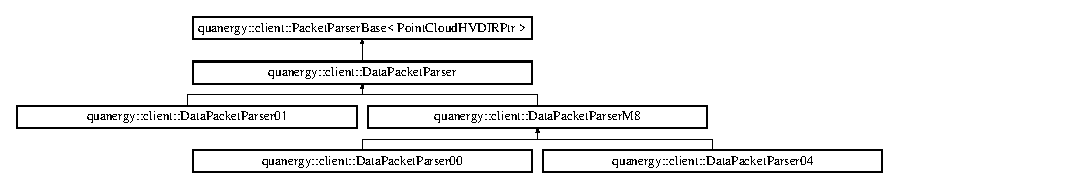
\includegraphics[height=2.085661cm]{structquanergy_1_1client_1_1DataPacketParser}
\end{center}
\end{figure}
\subsection*{Public Member Functions}
\begin{DoxyCompactItemize}
\item 
\hypertarget{structquanergy_1_1client_1_1DataPacketParser_a4aa6b9daacb64ba0b86c175fcc0a1d2b}{void \hyperlink{structquanergy_1_1client_1_1DataPacketParser_a4aa6b9daacb64ba0b86c175fcc0a1d2b}{set\-Frame\-Id} (const std\-::string frame\-\_\-id)}\label{structquanergy_1_1client_1_1DataPacketParser_a4aa6b9daacb64ba0b86c175fcc0a1d2b}

\begin{DoxyCompactList}\small\item\em common interface for setting frame\-\_\-id which should be put into resulting pointcloud \end{DoxyCompactList}\end{DoxyCompactItemize}
\subsection*{Protected Attributes}
\begin{DoxyCompactItemize}
\item 
\hypertarget{structquanergy_1_1client_1_1DataPacketParser_af52f9f1c410e1aa0adc40e024cece5b8}{std\-::string {\bfseries frame\-\_\-id\-\_\-}}\label{structquanergy_1_1client_1_1DataPacketParser_af52f9f1c410e1aa0adc40e024cece5b8}

\end{DoxyCompactItemize}


\subsection{Detailed Description}
base class for data packet parsers 

The documentation for this struct was generated from the following file\-:\begin{DoxyCompactItemize}
\item 
\hyperlink{data__packet__parser_8h}{data\-\_\-packet\-\_\-parser.\-h}\end{DoxyCompactItemize}

\hypertarget{structquanergy_1_1client_1_1DataPacketParser00}{\section{quanergy\-:\-:client\-:\-:Data\-Packet\-Parser00 Struct Reference}
\label{structquanergy_1_1client_1_1DataPacketParser00}\index{quanergy\-::client\-::\-Data\-Packet\-Parser00@{quanergy\-::client\-::\-Data\-Packet\-Parser00}}
}
Inheritance diagram for quanergy\-:\-:client\-:\-:Data\-Packet\-Parser00\-:\begin{figure}[H]
\begin{center}
\leavevmode
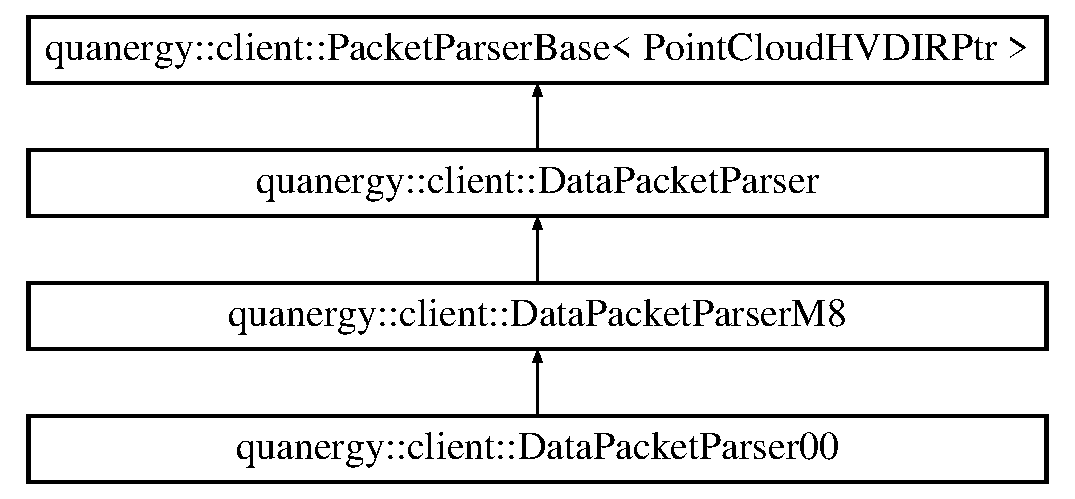
\includegraphics[height=4.000000cm]{structquanergy_1_1client_1_1DataPacketParser00}
\end{center}
\end{figure}
\subsection*{Public Member Functions}
\begin{DoxyCompactItemize}
\item 
virtual bool \hyperlink{structquanergy_1_1client_1_1DataPacketParser00_ac161241641118826d0514d293f7d6538}{validate} (const std\-::vector$<$ char $>$ \&packet)
\begin{DoxyCompactList}\small\item\em check packet validity \end{DoxyCompactList}\item 
virtual bool \hyperlink{structquanergy_1_1client_1_1DataPacketParser00_aceab95c7e5553724883adad72485d080}{parse} (const std\-::vector$<$ char $>$ \&packet, Point\-Cloud\-H\-V\-D\-I\-R\-Ptr \&result)
\begin{DoxyCompactList}\small\item\em parse packet and update result \end{DoxyCompactList}\end{DoxyCompactItemize}
\subsection*{Additional Inherited Members}


\subsection{Member Function Documentation}
\hypertarget{structquanergy_1_1client_1_1DataPacketParser00_aceab95c7e5553724883adad72485d080}{\index{quanergy\-::client\-::\-Data\-Packet\-Parser00@{quanergy\-::client\-::\-Data\-Packet\-Parser00}!parse@{parse}}
\index{parse@{parse}!quanergy::client::DataPacketParser00@{quanergy\-::client\-::\-Data\-Packet\-Parser00}}
\subsubsection[{parse}]{\setlength{\rightskip}{0pt plus 5cm}virtual bool quanergy\-::client\-::\-Data\-Packet\-Parser00\-::parse (
\begin{DoxyParamCaption}
\item[{const std\-::vector$<$ char $>$ \&}]{packet, }
\item[{Point\-Cloud\-H\-V\-D\-I\-R\-Ptr \&}]{result}
\end{DoxyParamCaption}
)\hspace{0.3cm}{\ttfamily [virtual]}}}\label{structquanergy_1_1client_1_1DataPacketParser00_aceab95c7e5553724883adad72485d080}


parse packet and update result 

\begin{DoxyReturn}{Returns}
true if result updated; false otherwise (some parsers may require multiple packets before updating result) 
\end{DoxyReturn}


Implements \hyperlink{structquanergy_1_1client_1_1PacketParserBase_a4a0555355f550738007edf7994da1c8c}{quanergy\-::client\-::\-Packet\-Parser\-Base$<$ Point\-Cloud\-H\-V\-D\-I\-R\-Ptr $>$}.

\hypertarget{structquanergy_1_1client_1_1DataPacketParser00_ac161241641118826d0514d293f7d6538}{\index{quanergy\-::client\-::\-Data\-Packet\-Parser00@{quanergy\-::client\-::\-Data\-Packet\-Parser00}!validate@{validate}}
\index{validate@{validate}!quanergy::client::DataPacketParser00@{quanergy\-::client\-::\-Data\-Packet\-Parser00}}
\subsubsection[{validate}]{\setlength{\rightskip}{0pt plus 5cm}virtual bool quanergy\-::client\-::\-Data\-Packet\-Parser00\-::validate (
\begin{DoxyParamCaption}
\item[{const std\-::vector$<$ char $>$ \&}]{packet}
\end{DoxyParamCaption}
)\hspace{0.3cm}{\ttfamily [virtual]}}}\label{structquanergy_1_1client_1_1DataPacketParser00_ac161241641118826d0514d293f7d6538}


check packet validity 

\begin{DoxyReturn}{Returns}
true if valid, false otherwise 
\end{DoxyReturn}


Implements \hyperlink{structquanergy_1_1client_1_1PacketParserBase_ad840fd4e7f3ab054024957ae1d94ffa1}{quanergy\-::client\-::\-Packet\-Parser\-Base$<$ Point\-Cloud\-H\-V\-D\-I\-R\-Ptr $>$}.



The documentation for this struct was generated from the following file\-:\begin{DoxyCompactItemize}
\item 
\hyperlink{data__packet__parser__00_8h}{data\-\_\-packet\-\_\-parser\-\_\-00.\-h}\end{DoxyCompactItemize}

\hypertarget{structquanergy_1_1client_1_1DataPacketParser01}{\section{quanergy\-:\-:client\-:\-:Data\-Packet\-Parser01 Struct Reference}
\label{structquanergy_1_1client_1_1DataPacketParser01}\index{quanergy\-::client\-::\-Data\-Packet\-Parser01@{quanergy\-::client\-::\-Data\-Packet\-Parser01}}
}
Inheritance diagram for quanergy\-:\-:client\-:\-:Data\-Packet\-Parser01\-:\begin{figure}[H]
\begin{center}
\leavevmode
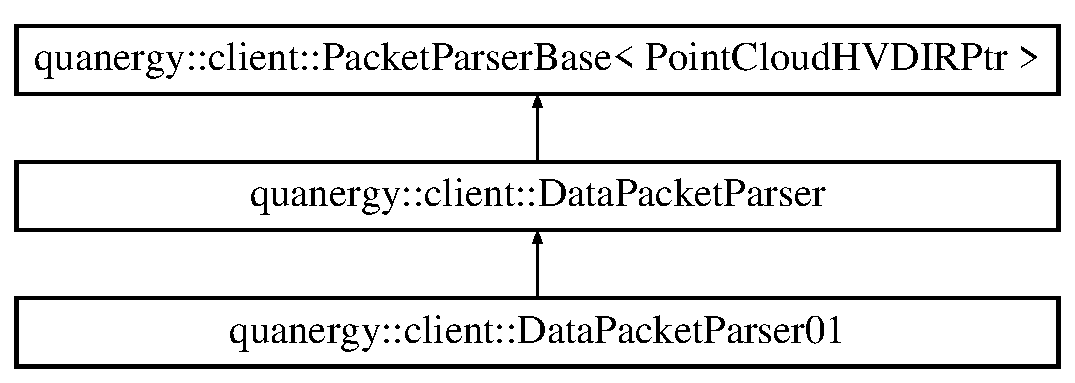
\includegraphics[height=3.000000cm]{structquanergy_1_1client_1_1DataPacketParser01}
\end{center}
\end{figure}
\subsection*{Public Member Functions}
\begin{DoxyCompactItemize}
\item 
virtual bool \hyperlink{structquanergy_1_1client_1_1DataPacketParser01_a0a28a9b2fecdd1cbb0afb8df05e1f90e}{validate} (const std\-::vector$<$ char $>$ \&packet)
\begin{DoxyCompactList}\small\item\em check packet validity \end{DoxyCompactList}\item 
virtual bool \hyperlink{structquanergy_1_1client_1_1DataPacketParser01_a5873c64ebd1b6261e6c6ec8694ab0061}{parse} (const std\-::vector$<$ char $>$ \&packet, Point\-Cloud\-H\-V\-D\-I\-R\-Ptr \&result)
\begin{DoxyCompactList}\small\item\em parse packet and update result \end{DoxyCompactList}\end{DoxyCompactItemize}
\subsection*{Additional Inherited Members}


\subsection{Member Function Documentation}
\hypertarget{structquanergy_1_1client_1_1DataPacketParser01_a5873c64ebd1b6261e6c6ec8694ab0061}{\index{quanergy\-::client\-::\-Data\-Packet\-Parser01@{quanergy\-::client\-::\-Data\-Packet\-Parser01}!parse@{parse}}
\index{parse@{parse}!quanergy::client::DataPacketParser01@{quanergy\-::client\-::\-Data\-Packet\-Parser01}}
\subsubsection[{parse}]{\setlength{\rightskip}{0pt plus 5cm}virtual bool quanergy\-::client\-::\-Data\-Packet\-Parser01\-::parse (
\begin{DoxyParamCaption}
\item[{const std\-::vector$<$ char $>$ \&}]{packet, }
\item[{Point\-Cloud\-H\-V\-D\-I\-R\-Ptr \&}]{result}
\end{DoxyParamCaption}
)\hspace{0.3cm}{\ttfamily [virtual]}}}\label{structquanergy_1_1client_1_1DataPacketParser01_a5873c64ebd1b6261e6c6ec8694ab0061}


parse packet and update result 

\begin{DoxyReturn}{Returns}
true if result updated; false otherwise (some parsers may require multiple packets before updating result) 
\end{DoxyReturn}


Implements \hyperlink{structquanergy_1_1client_1_1PacketParserBase_a4a0555355f550738007edf7994da1c8c}{quanergy\-::client\-::\-Packet\-Parser\-Base$<$ Point\-Cloud\-H\-V\-D\-I\-R\-Ptr $>$}.

\hypertarget{structquanergy_1_1client_1_1DataPacketParser01_a0a28a9b2fecdd1cbb0afb8df05e1f90e}{\index{quanergy\-::client\-::\-Data\-Packet\-Parser01@{quanergy\-::client\-::\-Data\-Packet\-Parser01}!validate@{validate}}
\index{validate@{validate}!quanergy::client::DataPacketParser01@{quanergy\-::client\-::\-Data\-Packet\-Parser01}}
\subsubsection[{validate}]{\setlength{\rightskip}{0pt plus 5cm}virtual bool quanergy\-::client\-::\-Data\-Packet\-Parser01\-::validate (
\begin{DoxyParamCaption}
\item[{const std\-::vector$<$ char $>$ \&}]{packet}
\end{DoxyParamCaption}
)\hspace{0.3cm}{\ttfamily [virtual]}}}\label{structquanergy_1_1client_1_1DataPacketParser01_a0a28a9b2fecdd1cbb0afb8df05e1f90e}


check packet validity 

\begin{DoxyReturn}{Returns}
true if valid, false otherwise 
\end{DoxyReturn}


Implements \hyperlink{structquanergy_1_1client_1_1PacketParserBase_ad840fd4e7f3ab054024957ae1d94ffa1}{quanergy\-::client\-::\-Packet\-Parser\-Base$<$ Point\-Cloud\-H\-V\-D\-I\-R\-Ptr $>$}.



The documentation for this struct was generated from the following file\-:\begin{DoxyCompactItemize}
\item 
\hyperlink{data__packet__parser__01_8h}{data\-\_\-packet\-\_\-parser\-\_\-01.\-h}\end{DoxyCompactItemize}

\hypertarget{structquanergy_1_1client_1_1DataPacketParser04}{\section{quanergy\-:\-:client\-:\-:Data\-Packet\-Parser04 Struct Reference}
\label{structquanergy_1_1client_1_1DataPacketParser04}\index{quanergy\-::client\-::\-Data\-Packet\-Parser04@{quanergy\-::client\-::\-Data\-Packet\-Parser04}}
}
Inheritance diagram for quanergy\-:\-:client\-:\-:Data\-Packet\-Parser04\-:\begin{figure}[H]
\begin{center}
\leavevmode
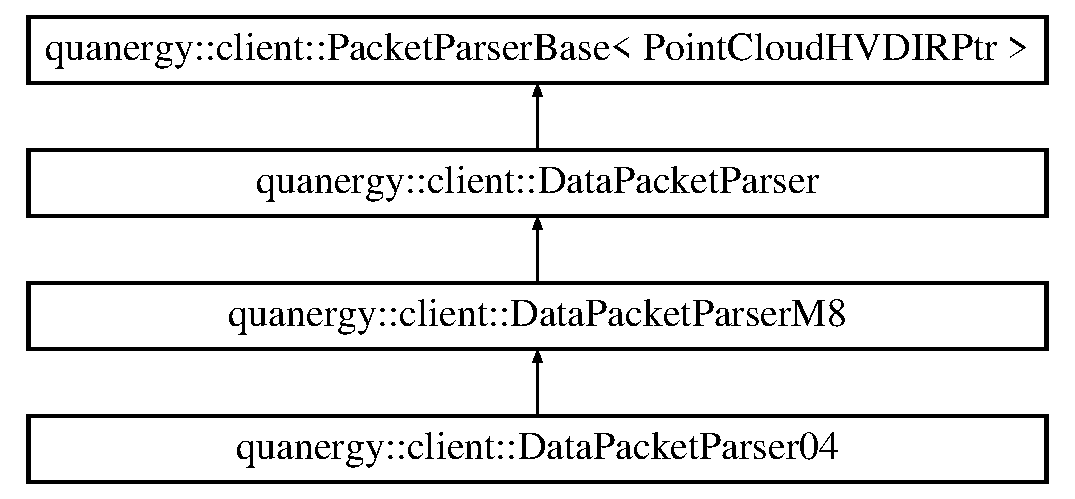
\includegraphics[height=4.000000cm]{structquanergy_1_1client_1_1DataPacketParser04}
\end{center}
\end{figure}
\subsection*{Public Member Functions}
\begin{DoxyCompactItemize}
\item 
bool \hyperlink{structquanergy_1_1client_1_1DataPacketParser04_a4f8566ff529171e458ab2139c9098403}{validate} (const std\-::vector$<$ char $>$ \&packet)
\begin{DoxyCompactList}\small\item\em check packet validity \end{DoxyCompactList}\item 
\hypertarget{structquanergy_1_1client_1_1DataPacketParser04_aa4d5c0f05ceb47c1fa5abdbb2a6ceae1}{bool {\bfseries parse} (\hyperlink{structquanergy_1_1client_1_1DataPacket04}{Data\-Packet04} const \&data\-\_\-packet, Point\-Cloud\-H\-V\-D\-I\-R\-Ptr \&result)}\label{structquanergy_1_1client_1_1DataPacketParser04_aa4d5c0f05ceb47c1fa5abdbb2a6ceae1}

\item 
bool \hyperlink{structquanergy_1_1client_1_1DataPacketParser04_a62df767eabc53340282c4f3cb5fec9e0}{parse} (const std\-::vector$<$ char $>$ \&packet, Point\-Cloud\-H\-V\-D\-I\-R\-Ptr \&result)
\begin{DoxyCompactList}\small\item\em parse packet and update result \end{DoxyCompactList}\end{DoxyCompactItemize}
\subsection*{Additional Inherited Members}


\subsection{Member Function Documentation}
\hypertarget{structquanergy_1_1client_1_1DataPacketParser04_a62df767eabc53340282c4f3cb5fec9e0}{\index{quanergy\-::client\-::\-Data\-Packet\-Parser04@{quanergy\-::client\-::\-Data\-Packet\-Parser04}!parse@{parse}}
\index{parse@{parse}!quanergy::client::DataPacketParser04@{quanergy\-::client\-::\-Data\-Packet\-Parser04}}
\subsubsection[{parse}]{\setlength{\rightskip}{0pt plus 5cm}bool quanergy\-::client\-::\-Data\-Packet\-Parser04\-::parse (
\begin{DoxyParamCaption}
\item[{const std\-::vector$<$ char $>$ \&}]{packet, }
\item[{Point\-Cloud\-H\-V\-D\-I\-R\-Ptr \&}]{result}
\end{DoxyParamCaption}
)\hspace{0.3cm}{\ttfamily [virtual]}}}\label{structquanergy_1_1client_1_1DataPacketParser04_a62df767eabc53340282c4f3cb5fec9e0}


parse packet and update result 

\begin{DoxyReturn}{Returns}
true if result updated; false otherwise (some parsers may require multiple packets before updating result) 
\end{DoxyReturn}


Implements \hyperlink{structquanergy_1_1client_1_1PacketParserBase_a4a0555355f550738007edf7994da1c8c}{quanergy\-::client\-::\-Packet\-Parser\-Base$<$ Point\-Cloud\-H\-V\-D\-I\-R\-Ptr $>$}.

\hypertarget{structquanergy_1_1client_1_1DataPacketParser04_a4f8566ff529171e458ab2139c9098403}{\index{quanergy\-::client\-::\-Data\-Packet\-Parser04@{quanergy\-::client\-::\-Data\-Packet\-Parser04}!validate@{validate}}
\index{validate@{validate}!quanergy::client::DataPacketParser04@{quanergy\-::client\-::\-Data\-Packet\-Parser04}}
\subsubsection[{validate}]{\setlength{\rightskip}{0pt plus 5cm}bool quanergy\-::client\-::\-Data\-Packet\-Parser04\-::validate (
\begin{DoxyParamCaption}
\item[{const std\-::vector$<$ char $>$ \&}]{packet}
\end{DoxyParamCaption}
)\hspace{0.3cm}{\ttfamily [virtual]}}}\label{structquanergy_1_1client_1_1DataPacketParser04_a4f8566ff529171e458ab2139c9098403}


check packet validity 

\begin{DoxyReturn}{Returns}
true if valid, false otherwise 
\end{DoxyReturn}


Implements \hyperlink{structquanergy_1_1client_1_1PacketParserBase_ad840fd4e7f3ab054024957ae1d94ffa1}{quanergy\-::client\-::\-Packet\-Parser\-Base$<$ Point\-Cloud\-H\-V\-D\-I\-R\-Ptr $>$}.



The documentation for this struct was generated from the following file\-:\begin{DoxyCompactItemize}
\item 
\hyperlink{data__packet__parser__04_8h}{data\-\_\-packet\-\_\-parser\-\_\-04.\-h}\end{DoxyCompactItemize}

\hypertarget{structquanergy_1_1client_1_1DataPacketParserM8}{\section{quanergy\-:\-:client\-:\-:Data\-Packet\-Parser\-M8 Struct Reference}
\label{structquanergy_1_1client_1_1DataPacketParserM8}\index{quanergy\-::client\-::\-Data\-Packet\-Parser\-M8@{quanergy\-::client\-::\-Data\-Packet\-Parser\-M8}}
}


Not a specialization because it is intended to be used by others.  




{\ttfamily \#include $<$data\-\_\-packet\-\_\-parser\-\_\-m8.\-h$>$}

Inheritance diagram for quanergy\-:\-:client\-:\-:Data\-Packet\-Parser\-M8\-:\begin{figure}[H]
\begin{center}
\leavevmode
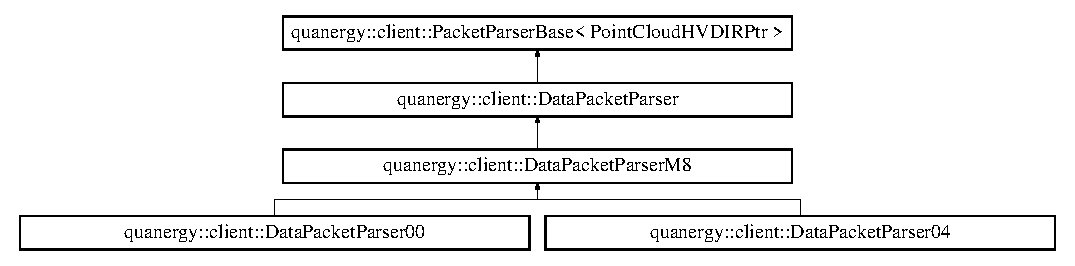
\includegraphics[height=3.128492cm]{structquanergy_1_1client_1_1DataPacketParserM8}
\end{center}
\end{figure}
\subsection*{Public Member Functions}
\begin{DoxyCompactItemize}
\item 
\hypertarget{structquanergy_1_1client_1_1DataPacketParserM8_a3d55d291d44be412eb30982c109c9b26}{bool {\bfseries parse} (const \hyperlink{structquanergy_1_1client_1_1M8DataPacket}{M8\-Data\-Packet} \&data\-\_\-packet, Point\-Cloud\-H\-V\-D\-I\-R\-Ptr \&result)}\label{structquanergy_1_1client_1_1DataPacketParserM8_a3d55d291d44be412eb30982c109c9b26}

\item 
\hypertarget{structquanergy_1_1client_1_1DataPacketParserM8_aff75b6e5c7965909ac77080f289770b8}{void {\bfseries set\-Return\-Selection} (int return\-\_\-selection)}\label{structquanergy_1_1client_1_1DataPacketParserM8_aff75b6e5c7965909ac77080f289770b8}

\item 
\hypertarget{structquanergy_1_1client_1_1DataPacketParserM8_a6f64769dfea51dbc43691f5ff43e8b0b}{void {\bfseries set\-Cloud\-Size\-Limits} (std\-::int32\-\_\-t szmin, std\-::int32\-\_\-t szmax)}\label{structquanergy_1_1client_1_1DataPacketParserM8_a6f64769dfea51dbc43691f5ff43e8b0b}

\item 
\hypertarget{structquanergy_1_1client_1_1DataPacketParserM8_aea770e4f27886c7fff318fb72535ed8d}{void {\bfseries set\-Degrees\-Of\-Sweep\-Per\-Cloud} (double degrees\-\_\-per\-\_\-cloud)}\label{structquanergy_1_1client_1_1DataPacketParserM8_aea770e4f27886c7fff318fb72535ed8d}

\item 
\hypertarget{structquanergy_1_1client_1_1DataPacketParserM8_ae919de33ff1688037d4aff2a5c668284}{double {\bfseries get\-Degrees\-Of\-Sweep\-Per\-Cloud} () const }\label{structquanergy_1_1client_1_1DataPacketParserM8_ae919de33ff1688037d4aff2a5c668284}

\end{DoxyCompactItemize}
\subsection*{Static Protected Member Functions}
\begin{DoxyCompactItemize}
\item 
\hypertarget{structquanergy_1_1client_1_1DataPacketParserM8_a07831058de6fe2804b51d6a1ff9394c4}{static void {\bfseries organize\-Cloud} (Point\-Cloud\-H\-V\-D\-I\-R\-Ptr \&current\-\_\-pc, Point\-Cloud\-H\-V\-D\-I\-R\-Ptr \&temp\-\_\-pc)}\label{structquanergy_1_1client_1_1DataPacketParserM8_a07831058de6fe2804b51d6a1ff9394c4}

\end{DoxyCompactItemize}
\subsection*{Protected Attributes}
\begin{DoxyCompactItemize}
\item 
\hypertarget{structquanergy_1_1client_1_1DataPacketParserM8_a6e7825f339f311dc6cf4fbad4d1df44b}{uint32\-\_\-t \hyperlink{structquanergy_1_1client_1_1DataPacketParserM8_a6e7825f339f311dc6cf4fbad4d1df44b}{packet\-\_\-counter\-\_\-}}\label{structquanergy_1_1client_1_1DataPacketParserM8_a6e7825f339f311dc6cf4fbad4d1df44b}

\begin{DoxyCompactList}\small\item\em global packet counter \end{DoxyCompactList}\item 
\hypertarget{structquanergy_1_1client_1_1DataPacketParserM8_aac2fa9bb2410d065a16cb32458d134b3}{uint32\-\_\-t \hyperlink{structquanergy_1_1client_1_1DataPacketParserM8_aac2fa9bb2410d065a16cb32458d134b3}{cloud\-\_\-counter\-\_\-}}\label{structquanergy_1_1client_1_1DataPacketParserM8_aac2fa9bb2410d065a16cb32458d134b3}

\begin{DoxyCompactList}\small\item\em global cloud counter \end{DoxyCompactList}\item 
\hypertarget{structquanergy_1_1client_1_1DataPacketParserM8_a58460ac04bc0d7bc1b410e09a06e5692}{double \hyperlink{structquanergy_1_1client_1_1DataPacketParserM8_a58460ac04bc0d7bc1b410e09a06e5692}{last\-\_\-azimuth\-\_\-}}\label{structquanergy_1_1client_1_1DataPacketParserM8_a58460ac04bc0d7bc1b410e09a06e5692}

\begin{DoxyCompactList}\small\item\em last accounted for azimuth angle \end{DoxyCompactList}\item 
\hypertarget{structquanergy_1_1client_1_1DataPacketParserM8_a1edb9bd53f79f9bc0af0772dc08726d2}{std\-::uint64\-\_\-t \hyperlink{structquanergy_1_1client_1_1DataPacketParserM8_a1edb9bd53f79f9bc0af0772dc08726d2}{previous\-\_\-packet\-\_\-stamp\-\_\-} = 0}\label{structquanergy_1_1client_1_1DataPacketParserM8_a1edb9bd53f79f9bc0af0772dc08726d2}

\begin{DoxyCompactList}\small\item\em timestamp of previous data packet (microseconds) \end{DoxyCompactList}\item 
\hypertarget{structquanergy_1_1client_1_1DataPacketParserM8_a6e32df4d489bc2989d57222eb0989f28}{Point\-Cloud\-H\-V\-D\-I\-R\-Ptr {\bfseries current\-\_\-cloud\-\_\-}}\label{structquanergy_1_1client_1_1DataPacketParserM8_a6e32df4d489bc2989d57222eb0989f28}

\item 
\hypertarget{structquanergy_1_1client_1_1DataPacketParserM8_aeb0372aa04c7848f9db3335a8d248658}{Point\-Cloud\-H\-V\-D\-I\-R\-Ptr {\bfseries worker\-\_\-cloud\-\_\-}}\label{structquanergy_1_1client_1_1DataPacketParserM8_aeb0372aa04c7848f9db3335a8d248658}

\item 
\hypertarget{structquanergy_1_1client_1_1DataPacketParserM8_a7fa907a63e2f43927540366f20a4c379}{std\-::vector$<$ double $>$ \hyperlink{structquanergy_1_1client_1_1DataPacketParserM8_a7fa907a63e2f43927540366f20a4c379}{horizontal\-\_\-angle\-\_\-lookup\-\_\-table\-\_\-}}\label{structquanergy_1_1client_1_1DataPacketParserM8_a7fa907a63e2f43927540366f20a4c379}

\begin{DoxyCompactList}\small\item\em lookup table for horizontal angle \end{DoxyCompactList}\item 
\hypertarget{structquanergy_1_1client_1_1DataPacketParserM8_a2f4b38c7647e7fc5196f82bd84b7b93d}{double \hyperlink{structquanergy_1_1client_1_1DataPacketParserM8_a2f4b38c7647e7fc5196f82bd84b7b93d}{vertical\-\_\-angle\-\_\-lookup\-\_\-table\-\_\-} \mbox{[}M8\-\_\-\-N\-U\-M\-\_\-\-L\-A\-S\-E\-R\-S\mbox{]}}\label{structquanergy_1_1client_1_1DataPacketParserM8_a2f4b38c7647e7fc5196f82bd84b7b93d}

\begin{DoxyCompactList}\small\item\em lookup table for vertical angle \end{DoxyCompactList}\item 
\hypertarget{structquanergy_1_1client_1_1DataPacketParserM8_adbfa45df9611f3aff9c94fef46c8129f}{int \hyperlink{structquanergy_1_1client_1_1DataPacketParserM8_adbfa45df9611f3aff9c94fef46c8129f}{return\-\_\-selection\-\_\-} = 0}\label{structquanergy_1_1client_1_1DataPacketParserM8_adbfa45df9611f3aff9c94fef46c8129f}

\begin{DoxyCompactList}\small\item\em return selection \end{DoxyCompactList}\item 
\hypertarget{structquanergy_1_1client_1_1DataPacketParserM8_ae1fe07e2deb0a1f81e94d1c19a45303b}{std\-::int32\-\_\-t \hyperlink{structquanergy_1_1client_1_1DataPacketParserM8_ae1fe07e2deb0a1f81e94d1c19a45303b}{minimum\-\_\-cloud\-\_\-size\-\_\-} = 1}\label{structquanergy_1_1client_1_1DataPacketParserM8_ae1fe07e2deb0a1f81e94d1c19a45303b}

\begin{DoxyCompactList}\small\item\em cloud size limits \end{DoxyCompactList}\item 
\hypertarget{structquanergy_1_1client_1_1DataPacketParserM8_a905ad66be49de4168f9997a8bd530f84}{std\-::int32\-\_\-t {\bfseries maximum\-\_\-cloud\-\_\-size\-\_\-} = 1\-E6}\label{structquanergy_1_1client_1_1DataPacketParserM8_a905ad66be49de4168f9997a8bd530f84}

\item 
\hypertarget{structquanergy_1_1client_1_1DataPacketParserM8_a595251e17f0542f93563398c2ccad31e}{double \hyperlink{structquanergy_1_1client_1_1DataPacketParserM8_a595251e17f0542f93563398c2ccad31e}{start\-\_\-azimuth\-\_\-}}\label{structquanergy_1_1client_1_1DataPacketParserM8_a595251e17f0542f93563398c2ccad31e}

\begin{DoxyCompactList}\small\item\em cloud degrees of sweep \end{DoxyCompactList}\item 
\hypertarget{structquanergy_1_1client_1_1DataPacketParserM8_a6c7c7adf5f968c6e59a505d4aa234fdc}{double {\bfseries degrees\-\_\-per\-\_\-cloud\-\_\-}}\label{structquanergy_1_1client_1_1DataPacketParserM8_a6c7c7adf5f968c6e59a505d4aa234fdc}

\item 
\hypertarget{structquanergy_1_1client_1_1DataPacketParserM8_a5f9e9890b2f0903472d9deedfa5031d9}{int \hyperlink{structquanergy_1_1client_1_1DataPacketParserM8_a5f9e9890b2f0903472d9deedfa5031d9}{direction\-\_\-} = 1}\label{structquanergy_1_1client_1_1DataPacketParserM8_a5f9e9890b2f0903472d9deedfa5031d9}

\begin{DoxyCompactList}\small\item\em direction \end{DoxyCompactList}\end{DoxyCompactItemize}


\subsection{Detailed Description}
Not a specialization because it is intended to be used by others. 

The documentation for this struct was generated from the following file\-:\begin{DoxyCompactItemize}
\item 
\hyperlink{data__packet__parser__m8_8h}{data\-\_\-packet\-\_\-parser\-\_\-m8.\-h}\end{DoxyCompactItemize}

\hypertarget{structquanergy_1_1client_1_1DataPoint01}{\section{quanergy\-:\-:client\-:\-:Data\-Point01 Struct Reference}
\label{structquanergy_1_1client_1_1DataPoint01}\index{quanergy\-::client\-::\-Data\-Point01@{quanergy\-::client\-::\-Data\-Point01}}
}


data point 0x01  




{\ttfamily \#include $<$data\-\_\-packet\-\_\-01.\-h$>$}

\subsection*{Public Attributes}
\begin{DoxyCompactItemize}
\item 
\hypertarget{structquanergy_1_1client_1_1DataPoint01_a12c6c56981db3dca0fbbc82a22fa408f}{std\-::int16\-\_\-t {\bfseries horizontal\-\_\-angle}}\label{structquanergy_1_1client_1_1DataPoint01_a12c6c56981db3dca0fbbc82a22fa408f}

\item 
\hypertarget{structquanergy_1_1client_1_1DataPoint01_a1e0a54d88a120aafb787f2039b15a286}{std\-::int16\-\_\-t {\bfseries vertical\-\_\-angle}}\label{structquanergy_1_1client_1_1DataPoint01_a1e0a54d88a120aafb787f2039b15a286}

\item 
\hypertarget{structquanergy_1_1client_1_1DataPoint01_ab6f942353ba69e35cc44f5e08d6db0b4}{std\-::uint32\-\_\-t {\bfseries range}}\label{structquanergy_1_1client_1_1DataPoint01_ab6f942353ba69e35cc44f5e08d6db0b4}

\item 
\hypertarget{structquanergy_1_1client_1_1DataPoint01_a52b701b904c3651a77ca803e5877a870}{std\-::uint16\-\_\-t {\bfseries intensity}}\label{structquanergy_1_1client_1_1DataPoint01_a52b701b904c3651a77ca803e5877a870}

\item 
\hypertarget{structquanergy_1_1client_1_1DataPoint01_a505fcd319dc02759aff13b713e21e1fc}{std\-::uint8\-\_\-t {\bfseries status}}\label{structquanergy_1_1client_1_1DataPoint01_a505fcd319dc02759aff13b713e21e1fc}

\item 
\hypertarget{structquanergy_1_1client_1_1DataPoint01_abc240b9f69302356ab0514bb6578366d}{std\-::uint8\-\_\-t {\bfseries reserved}}\label{structquanergy_1_1client_1_1DataPoint01_abc240b9f69302356ab0514bb6578366d}

\end{DoxyCompactItemize}


\subsection{Detailed Description}
data point 0x01 

The documentation for this struct was generated from the following file\-:\begin{DoxyCompactItemize}
\item 
\hyperlink{data__packet__01_8h}{data\-\_\-packet\-\_\-01.\-h}\end{DoxyCompactItemize}

\hypertarget{structquanergy_1_1client_1_1DistanceFilter}{\section{quanergy\-:\-:client\-:\-:Distance\-Filter Struct Reference}
\label{structquanergy_1_1client_1_1DistanceFilter}\index{quanergy\-::client\-::\-Distance\-Filter@{quanergy\-::client\-::\-Distance\-Filter}}
}
\subsection*{Public Types}
\begin{DoxyCompactItemize}
\item 
\hypertarget{structquanergy_1_1client_1_1DistanceFilter_a50f0687f568ce3ebcb3ede06f1682a11}{typedef std\-::shared\-\_\-ptr\\*
$<$ \hyperlink{structquanergy_1_1client_1_1DistanceFilter}{Distance\-Filter} $>$ {\bfseries Ptr}}\label{structquanergy_1_1client_1_1DistanceFilter_a50f0687f568ce3ebcb3ede06f1682a11}

\item 
\hypertarget{structquanergy_1_1client_1_1DistanceFilter_a592ba10aafe5178333c6ea0001c9e760}{typedef Point\-Cloud\-H\-V\-D\-I\-R\-Ptr {\bfseries Result\-Type}}\label{structquanergy_1_1client_1_1DistanceFilter_a592ba10aafe5178333c6ea0001c9e760}

\item 
\hypertarget{structquanergy_1_1client_1_1DistanceFilter_a95ae0d3f4bc572a61bf85a805448210b}{typedef \\*
boost\-::signals2\-::signal$<$ void(const \\*
Result\-Type \&)$>$ {\bfseries Signal}}\label{structquanergy_1_1client_1_1DistanceFilter_a95ae0d3f4bc572a61bf85a805448210b}

\end{DoxyCompactItemize}
\subsection*{Public Member Functions}
\begin{DoxyCompactItemize}
\item 
\hypertarget{structquanergy_1_1client_1_1DistanceFilter_a745c27681eef00dfc11c06b53c9a9217}{boost\-::signals2\-::connection {\bfseries connect} (const T\-Y\-P\-E\-N\-A\-M\-E Signal\-::slot\-\_\-type \&subscriber)}\label{structquanergy_1_1client_1_1DistanceFilter_a745c27681eef00dfc11c06b53c9a9217}

\item 
\hypertarget{structquanergy_1_1client_1_1DistanceFilter_a27a0f321664669d9254cad2ffe0cbdbc}{void {\bfseries slot} (Point\-Cloud\-H\-V\-D\-I\-R\-Const\-Ptr const \&)}\label{structquanergy_1_1client_1_1DistanceFilter_a27a0f321664669d9254cad2ffe0cbdbc}

\item 
\hypertarget{structquanergy_1_1client_1_1DistanceFilter_a76be8a90183cf5918c75f4d970101b2e}{void {\bfseries set\-Maximum\-Distance\-Threshold} (float max\-Threshold)}\label{structquanergy_1_1client_1_1DistanceFilter_a76be8a90183cf5918c75f4d970101b2e}

\item 
\hypertarget{structquanergy_1_1client_1_1DistanceFilter_a65f44c8186494496689956f5dd49ab29}{float {\bfseries get\-Maximum\-Distance\-Threshold} () const }\label{structquanergy_1_1client_1_1DistanceFilter_a65f44c8186494496689956f5dd49ab29}

\item 
\hypertarget{structquanergy_1_1client_1_1DistanceFilter_ad8dd4bee3ac8685006a290c59faf455d}{void {\bfseries set\-Minimum\-Distance\-Threshold} (float min\-Threshold)}\label{structquanergy_1_1client_1_1DistanceFilter_ad8dd4bee3ac8685006a290c59faf455d}

\item 
\hypertarget{structquanergy_1_1client_1_1DistanceFilter_a325f497b8fe2438f8f19877819aca89d}{float {\bfseries get\-Minimum\-Distance\-Threshold} () const }\label{structquanergy_1_1client_1_1DistanceFilter_a325f497b8fe2438f8f19877819aca89d}

\end{DoxyCompactItemize}


The documentation for this struct was generated from the following file\-:\begin{DoxyCompactItemize}
\item 
\hyperlink{distance__filter_8h}{distance\-\_\-filter.\-h}\end{DoxyCompactItemize}

\hypertarget{structquanergy_1_1calibration_1_1EncoderAngleCalibration}{\section{quanergy\-:\-:calibration\-:\-:Encoder\-Angle\-Calibration Struct Reference}
\label{structquanergy_1_1calibration_1_1EncoderAngleCalibration}\index{quanergy\-::calibration\-::\-Encoder\-Angle\-Calibration@{quanergy\-::calibration\-::\-Encoder\-Angle\-Calibration}}
}


This class calculates the error in the encoder angles and returns the amplitude and phase shift of the sine function modeling the error in the encoder angles for the M8 Sensor. This class can also be provided with the sine error parameters and apply the calibration to incoming points.  




{\ttfamily \#include $<$encoder\-\_\-angle\-\_\-calibration.\-h$>$}

\subsection*{Public Types}
\begin{DoxyCompactItemize}
\item 
using \hyperlink{structquanergy_1_1calibration_1_1EncoderAngleCalibration_ad2e08ae4ae94662029c907d43c5f879c}{Angle\-Container} = std\-::vector$<$ double $>$
\item 
using \hyperlink{structquanergy_1_1calibration_1_1EncoderAngleCalibration_a989e77cbef9730169908a437323a96c2}{Sine\-Parameters} = std\-::pair$<$ double, double $>$
\item 
using \hyperlink{structquanergy_1_1calibration_1_1EncoderAngleCalibration_aa41576cd5cbf0b1d917a9a781be9e308}{Line\-Parameters} = std\-::pair$<$ double, double $>$
\item 
\hypertarget{structquanergy_1_1calibration_1_1EncoderAngleCalibration_ae50457c8a6ce95e6c44c3aa32659ee40}{using \hyperlink{structquanergy_1_1calibration_1_1EncoderAngleCalibration_ae50457c8a6ce95e6c44c3aa32659ee40}{Ptr} = std\-::shared\-\_\-ptr$<$ \hyperlink{structquanergy_1_1calibration_1_1EncoderAngleCalibration}{Encoder\-Angle\-Calibration} $>$}\label{structquanergy_1_1calibration_1_1EncoderAngleCalibration_ae50457c8a6ce95e6c44c3aa32659ee40}

\begin{DoxyCompactList}\small\item\em Short-\/hand for point types. \end{DoxyCompactList}\item 
\hypertarget{structquanergy_1_1calibration_1_1EncoderAngleCalibration_a32f20fa67f6d6bff7b21b76f695489f7}{using \hyperlink{structquanergy_1_1calibration_1_1EncoderAngleCalibration_a32f20fa67f6d6bff7b21b76f695489f7}{Result\-Type} = Point\-Cloud\-H\-V\-D\-I\-R\-Ptr}\label{structquanergy_1_1calibration_1_1EncoderAngleCalibration_a32f20fa67f6d6bff7b21b76f695489f7}

\begin{DoxyCompactList}\small\item\em Result type for class. \end{DoxyCompactList}\item 
\hypertarget{structquanergy_1_1calibration_1_1EncoderAngleCalibration_aeb5bc875838932085c43143e44a2942a}{using \hyperlink{structquanergy_1_1calibration_1_1EncoderAngleCalibration_aeb5bc875838932085c43143e44a2942a}{Signal} = boost\-::signals2\-::signal$<$ void(const \hyperlink{structquanergy_1_1calibration_1_1EncoderAngleCalibration_a32f20fa67f6d6bff7b21b76f695489f7}{Result\-Type} \&)$>$}\label{structquanergy_1_1calibration_1_1EncoderAngleCalibration_aeb5bc875838932085c43143e44a2942a}

\begin{DoxyCompactList}\small\item\em Signal type. \end{DoxyCompactList}\end{DoxyCompactItemize}
\subsection*{Public Member Functions}
\begin{DoxyCompactItemize}
\item 
\hypertarget{structquanergy_1_1calibration_1_1EncoderAngleCalibration_a4c86719a8e5a36a1b14dba38e5bd4901}{\hyperlink{structquanergy_1_1calibration_1_1EncoderAngleCalibration_a4c86719a8e5a36a1b14dba38e5bd4901}{Encoder\-Angle\-Calibration} ()}\label{structquanergy_1_1calibration_1_1EncoderAngleCalibration_a4c86719a8e5a36a1b14dba38e5bd4901}

\begin{DoxyCompactList}\small\item\em Constructor. \end{DoxyCompactList}\item 
\hypertarget{structquanergy_1_1calibration_1_1EncoderAngleCalibration_a0fa758e2353874d4d8a2d49c28fce4ba}{\hyperlink{structquanergy_1_1calibration_1_1EncoderAngleCalibration_a0fa758e2353874d4d8a2d49c28fce4ba}{$\sim$\-Encoder\-Angle\-Calibration} ()}\label{structquanergy_1_1calibration_1_1EncoderAngleCalibration_a0fa758e2353874d4d8a2d49c28fce4ba}

\begin{DoxyCompactList}\small\item\em Empty destructor. \end{DoxyCompactList}\item 
boost\-::signals2\-::connection \hyperlink{structquanergy_1_1calibration_1_1EncoderAngleCalibration_a1b1d924f8633dcb48898c32d7fabf651}{connect} (const T\-Y\-P\-E\-N\-A\-M\-E Signal\-::slot\-\_\-type \&subscriber)
\begin{DoxyCompactList}\small\item\em Adds subscriber to be called after this classes functionality is done. \end{DoxyCompactList}\item 
void \hyperlink{structquanergy_1_1calibration_1_1EncoderAngleCalibration_ac73746735a610fe7f4b9a261f5eabf9f}{slot} (Point\-Cloud\-H\-V\-D\-I\-R\-Ptr const \&pc)
\begin{DoxyCompactList}\small\item\em Slot to be connected as a subscriber to another process. If calibration is not complete, this function will add the point cloud argument to the cloud to be used for calibration. If calibration is complete, this function will apply the calibration and call the next subscriber. \end{DoxyCompactList}\item 
\hypertarget{structquanergy_1_1calibration_1_1EncoderAngleCalibration_acd0f552b95aa74d0738d7c5d7e89d1fa}{void \hyperlink{structquanergy_1_1calibration_1_1EncoderAngleCalibration_acd0f552b95aa74d0738d7c5d7e89d1fa}{calibrate\-Only} ()}\label{structquanergy_1_1calibration_1_1EncoderAngleCalibration_acd0f552b95aa74d0738d7c5d7e89d1fa}

\begin{DoxyCompactList}\small\item\em Sets this class to only calculate the error parameters and not apply the calibration. This mode is for when the caller wants to look at multiple calculations for the amplitude and phase. \end{DoxyCompactList}\item 
void \hyperlink{structquanergy_1_1calibration_1_1EncoderAngleCalibration_aa86be4f4d781cad40afab05f40ad78d6}{set\-Required\-Num\-Samples} (double num\-\_\-cals)
\begin{DoxyCompactList}\small\item\em Sets number of valid calibrations to be collected before averaging. Validity is determined by change in phase between current sample and previous sample. \end{DoxyCompactList}\item 
void \hyperlink{structquanergy_1_1calibration_1_1EncoderAngleCalibration_a0f9d48e2c8ccaf03647dde2666985819}{set\-Params} (double amplitude, double phase)
\begin{DoxyCompactList}\small\item\em Function to manually set calibration parameters. Calling this function will disable the automatic calibration and subsequent calls to slot will apply the calibration and call the subscriber. \end{DoxyCompactList}\item 
void \hyperlink{structquanergy_1_1calibration_1_1EncoderAngleCalibration_a8fe3b279f9dbed5e17e91bbe4271943d}{set\-Frame\-Rate} (double frame\-\_\-rate)
\begin{DoxyCompactList}\small\item\em Function to set frame rate. Value is in frames per second. If not set, the default is 10. \end{DoxyCompactList}\item 
{\footnotesize template$<$typename Rep , typename Period $>$ }\\void \hyperlink{structquanergy_1_1calibration_1_1EncoderAngleCalibration_a478a432ee011bab690954869f8638ce1}{set\-Timeout} (const std\-::chrono\-::duration$<$ Rep, Period $>$ \&timeout)
\begin{DoxyCompactList}\small\item\em Sets timeout for calculating the calibration. If the timeout expires this class will throw an exception. \end{DoxyCompactList}\item 
\hyperlink{structquanergy_1_1calibration_1_1EncoderAngleCalibration_a989e77cbef9730169908a437323a96c2}{Sine\-Parameters} \hyperlink{structquanergy_1_1calibration_1_1EncoderAngleCalibration_a2c4dc14bab7cad0d55e9466e044424a2}{calculate} (const std\-::vector$<$ double $>$ \&encoder\-\_\-angles)
\begin{DoxyCompactList}\small\item\em Function to calculate the sinusoidal error of the horizontal encoder values. This function is called once a full revolution of the encoder is captured. \end{DoxyCompactList}\end{DoxyCompactItemize}
\subsection*{Static Public Attributes}
\begin{DoxyCompactItemize}
\item 
static const double \hyperlink{structquanergy_1_1calibration_1_1EncoderAngleCalibration_a76aedeeacc4ac54b5fa1324a144abaf6}{F\-I\-R\-I\-N\-G\-\_\-\-R\-A\-T\-E}
\item 
static const int \hyperlink{structquanergy_1_1calibration_1_1EncoderAngleCalibration_a78466d125a2b3c71199e06bb8f433738}{E\-N\-C\-O\-D\-E\-R\-\_\-\-C\-O\-U\-N\-T\-\_\-\-T\-O\-L\-E\-R\-A\-N\-C\-E}
\item 
static const int \hyperlink{structquanergy_1_1calibration_1_1EncoderAngleCalibration_abe79c88a1e3a3e42796a225e34c1d67f}{M\-I\-N\-\_\-\-E\-N\-C\-O\-D\-E\-R\-\_\-\-A\-N\-G\-L\-E\-S\-\_\-\-P\-E\-R\-\_\-\-R\-E\-V}
\item 
static const int \hyperlink{structquanergy_1_1calibration_1_1EncoderAngleCalibration_ab42e578d8a1c168e7d75506faad03dc2}{M\-A\-X\-\_\-\-E\-N\-C\-O\-D\-E\-R\-\_\-\-A\-N\-G\-L\-E\-S\-\_\-\-P\-E\-R\-\_\-\-R\-E\-V}
\item 
static const double \hyperlink{structquanergy_1_1calibration_1_1EncoderAngleCalibration_a934b8f1f5c14ed61c7ba6bc5e01ddd5b}{P\-I\-\_\-\-T\-O\-L\-E\-R\-A\-N\-C\-E}
\item 
static const int \hyperlink{structquanergy_1_1calibration_1_1EncoderAngleCalibration_a0d42f1ff560d67d491511970960f0cfa}{M\-O\-V\-\_\-\-A\-V\-G\-\_\-\-P\-E\-R\-I\-O\-D}
\item 
static const double \hyperlink{structquanergy_1_1calibration_1_1EncoderAngleCalibration_a12436409c1f1f10f4c005e45fcfbfbf2}{P\-H\-A\-S\-E\-\_\-\-C\-O\-N\-V\-E\-R\-G\-E\-N\-C\-E\-\_\-\-T\-H\-R\-E\-S\-H\-O\-L\-D}
\item 
static const double \hyperlink{structquanergy_1_1calibration_1_1EncoderAngleCalibration_a1b9a418e7547fb16216a839a0f605b47}{A\-M\-P\-L\-I\-T\-U\-D\-E\-\_\-\-T\-H\-R\-E\-S\-H\-O\-L\-D}
\end{DoxyCompactItemize}


\subsection{Detailed Description}
This class calculates the error in the encoder angles and returns the amplitude and phase shift of the sine function modeling the error in the encoder angles for the M8 Sensor. This class can also be provided with the sine error parameters and apply the calibration to incoming points. 

\subsection{Member Typedef Documentation}
\hypertarget{structquanergy_1_1calibration_1_1EncoderAngleCalibration_ad2e08ae4ae94662029c907d43c5f879c}{\index{quanergy\-::calibration\-::\-Encoder\-Angle\-Calibration@{quanergy\-::calibration\-::\-Encoder\-Angle\-Calibration}!Angle\-Container@{Angle\-Container}}
\index{Angle\-Container@{Angle\-Container}!quanergy::calibration::EncoderAngleCalibration@{quanergy\-::calibration\-::\-Encoder\-Angle\-Calibration}}
\subsubsection[{Angle\-Container}]{\setlength{\rightskip}{0pt plus 5cm}using {\bf quanergy\-::calibration\-::\-Encoder\-Angle\-Calibration\-::\-Angle\-Container} =  std\-::vector$<$double$>$}}\label{structquanergy_1_1calibration_1_1EncoderAngleCalibration_ad2e08ae4ae94662029c907d43c5f879c}
The type of the container that contains the encoder angles \hypertarget{structquanergy_1_1calibration_1_1EncoderAngleCalibration_aa41576cd5cbf0b1d917a9a781be9e308}{\index{quanergy\-::calibration\-::\-Encoder\-Angle\-Calibration@{quanergy\-::calibration\-::\-Encoder\-Angle\-Calibration}!Line\-Parameters@{Line\-Parameters}}
\index{Line\-Parameters@{Line\-Parameters}!quanergy::calibration::EncoderAngleCalibration@{quanergy\-::calibration\-::\-Encoder\-Angle\-Calibration}}
\subsubsection[{Line\-Parameters}]{\setlength{\rightskip}{0pt plus 5cm}using {\bf quanergy\-::calibration\-::\-Encoder\-Angle\-Calibration\-::\-Line\-Parameters} =  std\-::pair$<$double, double$>$}}\label{structquanergy_1_1calibration_1_1EncoderAngleCalibration_aa41576cd5cbf0b1d917a9a781be9e308}
This type holds the parameters of a 2d line \hypertarget{structquanergy_1_1calibration_1_1EncoderAngleCalibration_a989e77cbef9730169908a437323a96c2}{\index{quanergy\-::calibration\-::\-Encoder\-Angle\-Calibration@{quanergy\-::calibration\-::\-Encoder\-Angle\-Calibration}!Sine\-Parameters@{Sine\-Parameters}}
\index{Sine\-Parameters@{Sine\-Parameters}!quanergy::calibration::EncoderAngleCalibration@{quanergy\-::calibration\-::\-Encoder\-Angle\-Calibration}}
\subsubsection[{Sine\-Parameters}]{\setlength{\rightskip}{0pt plus 5cm}using {\bf quanergy\-::calibration\-::\-Encoder\-Angle\-Calibration\-::\-Sine\-Parameters} =  std\-::pair$<$double, double$>$}}\label{structquanergy_1_1calibration_1_1EncoderAngleCalibration_a989e77cbef9730169908a437323a96c2}
This type holds the parameters of the sine wave. The amplitude is the first element of the pair, the phase is the second element. 

\subsection{Member Function Documentation}
\hypertarget{structquanergy_1_1calibration_1_1EncoderAngleCalibration_a2c4dc14bab7cad0d55e9466e044424a2}{\index{quanergy\-::calibration\-::\-Encoder\-Angle\-Calibration@{quanergy\-::calibration\-::\-Encoder\-Angle\-Calibration}!calculate@{calculate}}
\index{calculate@{calculate}!quanergy::calibration::EncoderAngleCalibration@{quanergy\-::calibration\-::\-Encoder\-Angle\-Calibration}}
\subsubsection[{calculate}]{\setlength{\rightskip}{0pt plus 5cm}{\bf Sine\-Parameters} quanergy\-::calibration\-::\-Encoder\-Angle\-Calibration\-::calculate (
\begin{DoxyParamCaption}
\item[{const std\-::vector$<$ double $>$ \&}]{encoder\-\_\-angles}
\end{DoxyParamCaption}
)}}\label{structquanergy_1_1calibration_1_1EncoderAngleCalibration_a2c4dc14bab7cad0d55e9466e044424a2}


Function to calculate the sinusoidal error of the horizontal encoder values. This function is called once a full revolution of the encoder is captured. 


\begin{DoxyParams}[1]{Parameters}
\mbox{\tt in}  & {\em encoder\-\_\-angles} & Encoder angles\\
\hline
\end{DoxyParams}
\begin{DoxyReturn}{Returns}
Tuple with first element as the amplitude of the sinusoid and second element as the phase offset of the sinusoid. 
\end{DoxyReturn}
\hypertarget{structquanergy_1_1calibration_1_1EncoderAngleCalibration_a1b1d924f8633dcb48898c32d7fabf651}{\index{quanergy\-::calibration\-::\-Encoder\-Angle\-Calibration@{quanergy\-::calibration\-::\-Encoder\-Angle\-Calibration}!connect@{connect}}
\index{connect@{connect}!quanergy::calibration::EncoderAngleCalibration@{quanergy\-::calibration\-::\-Encoder\-Angle\-Calibration}}
\subsubsection[{connect}]{\setlength{\rightskip}{0pt plus 5cm}boost\-::signals2\-::connection quanergy\-::calibration\-::\-Encoder\-Angle\-Calibration\-::connect (
\begin{DoxyParamCaption}
\item[{const T\-Y\-P\-E\-N\-A\-M\-E Signal\-::slot\-\_\-type \&}]{subscriber}
\end{DoxyParamCaption}
)}}\label{structquanergy_1_1calibration_1_1EncoderAngleCalibration_a1b1d924f8633dcb48898c32d7fabf651}


Adds subscriber to be called after this classes functionality is done. 


\begin{DoxyParams}[1]{Parameters}
\mbox{\tt in}  & {\em subscriber} & Subscriber to be called.\\
\hline
\end{DoxyParams}
\begin{DoxyReturn}{Returns}
connection between this class and subscriber 
\end{DoxyReturn}
\hypertarget{structquanergy_1_1calibration_1_1EncoderAngleCalibration_a8fe3b279f9dbed5e17e91bbe4271943d}{\index{quanergy\-::calibration\-::\-Encoder\-Angle\-Calibration@{quanergy\-::calibration\-::\-Encoder\-Angle\-Calibration}!set\-Frame\-Rate@{set\-Frame\-Rate}}
\index{set\-Frame\-Rate@{set\-Frame\-Rate}!quanergy::calibration::EncoderAngleCalibration@{quanergy\-::calibration\-::\-Encoder\-Angle\-Calibration}}
\subsubsection[{set\-Frame\-Rate}]{\setlength{\rightskip}{0pt plus 5cm}void quanergy\-::calibration\-::\-Encoder\-Angle\-Calibration\-::set\-Frame\-Rate (
\begin{DoxyParamCaption}
\item[{double}]{frame\-\_\-rate}
\end{DoxyParamCaption}
)}}\label{structquanergy_1_1calibration_1_1EncoderAngleCalibration_a8fe3b279f9dbed5e17e91bbe4271943d}


Function to set frame rate. Value is in frames per second. If not set, the default is 10. 


\begin{DoxyParams}[1]{Parameters}
\mbox{\tt in}  & {\em frame\-\_\-rate} & frame rate. \\
\hline
\end{DoxyParams}
\hypertarget{structquanergy_1_1calibration_1_1EncoderAngleCalibration_a0f9d48e2c8ccaf03647dde2666985819}{\index{quanergy\-::calibration\-::\-Encoder\-Angle\-Calibration@{quanergy\-::calibration\-::\-Encoder\-Angle\-Calibration}!set\-Params@{set\-Params}}
\index{set\-Params@{set\-Params}!quanergy::calibration::EncoderAngleCalibration@{quanergy\-::calibration\-::\-Encoder\-Angle\-Calibration}}
\subsubsection[{set\-Params}]{\setlength{\rightskip}{0pt plus 5cm}void quanergy\-::calibration\-::\-Encoder\-Angle\-Calibration\-::set\-Params (
\begin{DoxyParamCaption}
\item[{double}]{amplitude, }
\item[{double}]{phase}
\end{DoxyParamCaption}
)}}\label{structquanergy_1_1calibration_1_1EncoderAngleCalibration_a0f9d48e2c8ccaf03647dde2666985819}


Function to manually set calibration parameters. Calling this function will disable the automatic calibration and subsequent calls to slot will apply the calibration and call the subscriber. 


\begin{DoxyParams}[1]{Parameters}
\mbox{\tt in}  & {\em amplitude} & Amplitude of sinusoid error \\
\hline
\mbox{\tt in}  & {\em phase} & Phase of sinusoidal error \\
\hline
\end{DoxyParams}
\hypertarget{structquanergy_1_1calibration_1_1EncoderAngleCalibration_aa86be4f4d781cad40afab05f40ad78d6}{\index{quanergy\-::calibration\-::\-Encoder\-Angle\-Calibration@{quanergy\-::calibration\-::\-Encoder\-Angle\-Calibration}!set\-Required\-Num\-Samples@{set\-Required\-Num\-Samples}}
\index{set\-Required\-Num\-Samples@{set\-Required\-Num\-Samples}!quanergy::calibration::EncoderAngleCalibration@{quanergy\-::calibration\-::\-Encoder\-Angle\-Calibration}}
\subsubsection[{set\-Required\-Num\-Samples}]{\setlength{\rightskip}{0pt plus 5cm}void quanergy\-::calibration\-::\-Encoder\-Angle\-Calibration\-::set\-Required\-Num\-Samples (
\begin{DoxyParamCaption}
\item[{double}]{num\-\_\-cals}
\end{DoxyParamCaption}
)}}\label{structquanergy_1_1calibration_1_1EncoderAngleCalibration_aa86be4f4d781cad40afab05f40ad78d6}


Sets number of valid calibrations to be collected before averaging. Validity is determined by change in phase between current sample and previous sample. 


\begin{DoxyParams}[1]{Parameters}
\mbox{\tt in}  & {\em num\-\_\-cals} & Number of calibrations \\
\hline
\end{DoxyParams}
\hypertarget{structquanergy_1_1calibration_1_1EncoderAngleCalibration_a478a432ee011bab690954869f8638ce1}{\index{quanergy\-::calibration\-::\-Encoder\-Angle\-Calibration@{quanergy\-::calibration\-::\-Encoder\-Angle\-Calibration}!set\-Timeout@{set\-Timeout}}
\index{set\-Timeout@{set\-Timeout}!quanergy::calibration::EncoderAngleCalibration@{quanergy\-::calibration\-::\-Encoder\-Angle\-Calibration}}
\subsubsection[{set\-Timeout}]{\setlength{\rightskip}{0pt plus 5cm}template$<$typename Rep , typename Period $>$ void quanergy\-::calibration\-::\-Encoder\-Angle\-Calibration\-::set\-Timeout (
\begin{DoxyParamCaption}
\item[{const std\-::chrono\-::duration$<$ Rep, Period $>$ \&}]{timeout}
\end{DoxyParamCaption}
)}}\label{structquanergy_1_1calibration_1_1EncoderAngleCalibration_a478a432ee011bab690954869f8638ce1}


Sets timeout for calculating the calibration. If the timeout expires this class will throw an exception. 


\begin{DoxyParams}[1]{Parameters}
\mbox{\tt in}  & {\em timeout} & Timeout. \\
\hline
\end{DoxyParams}
\hypertarget{structquanergy_1_1calibration_1_1EncoderAngleCalibration_ac73746735a610fe7f4b9a261f5eabf9f}{\index{quanergy\-::calibration\-::\-Encoder\-Angle\-Calibration@{quanergy\-::calibration\-::\-Encoder\-Angle\-Calibration}!slot@{slot}}
\index{slot@{slot}!quanergy::calibration::EncoderAngleCalibration@{quanergy\-::calibration\-::\-Encoder\-Angle\-Calibration}}
\subsubsection[{slot}]{\setlength{\rightskip}{0pt plus 5cm}void quanergy\-::calibration\-::\-Encoder\-Angle\-Calibration\-::slot (
\begin{DoxyParamCaption}
\item[{Point\-Cloud\-H\-V\-D\-I\-R\-Ptr const \&}]{pc}
\end{DoxyParamCaption}
)}}\label{structquanergy_1_1calibration_1_1EncoderAngleCalibration_ac73746735a610fe7f4b9a261f5eabf9f}


Slot to be connected as a subscriber to another process. If calibration is not complete, this function will add the point cloud argument to the cloud to be used for calibration. If calibration is complete, this function will apply the calibration and call the next subscriber. 


\begin{DoxyParams}[1]{Parameters}
\mbox{\tt in}  & {\em pc} & Point cloud to be processed. \\
\hline
\end{DoxyParams}


\subsection{Member Data Documentation}
\hypertarget{structquanergy_1_1calibration_1_1EncoderAngleCalibration_a1b9a418e7547fb16216a839a0f605b47}{\index{quanergy\-::calibration\-::\-Encoder\-Angle\-Calibration@{quanergy\-::calibration\-::\-Encoder\-Angle\-Calibration}!A\-M\-P\-L\-I\-T\-U\-D\-E\-\_\-\-T\-H\-R\-E\-S\-H\-O\-L\-D@{A\-M\-P\-L\-I\-T\-U\-D\-E\-\_\-\-T\-H\-R\-E\-S\-H\-O\-L\-D}}
\index{A\-M\-P\-L\-I\-T\-U\-D\-E\-\_\-\-T\-H\-R\-E\-S\-H\-O\-L\-D@{A\-M\-P\-L\-I\-T\-U\-D\-E\-\_\-\-T\-H\-R\-E\-S\-H\-O\-L\-D}!quanergy::calibration::EncoderAngleCalibration@{quanergy\-::calibration\-::\-Encoder\-Angle\-Calibration}}
\subsubsection[{A\-M\-P\-L\-I\-T\-U\-D\-E\-\_\-\-T\-H\-R\-E\-S\-H\-O\-L\-D}]{\setlength{\rightskip}{0pt plus 5cm}const double quanergy\-::calibration\-::\-Encoder\-Angle\-Calibration\-::\-A\-M\-P\-L\-I\-T\-U\-D\-E\-\_\-\-T\-H\-R\-E\-S\-H\-O\-L\-D\hspace{0.3cm}{\ttfamily [static]}}}\label{structquanergy_1_1calibration_1_1EncoderAngleCalibration_a1b9a418e7547fb16216a839a0f605b47}
Amplitude threshold dictating if calculating the encoder offset is appropriate. If an encoder calibration returns an amplitude below this value, this class indicates that calibration is complete and applies no calibration to outgoing points. \hypertarget{structquanergy_1_1calibration_1_1EncoderAngleCalibration_a78466d125a2b3c71199e06bb8f433738}{\index{quanergy\-::calibration\-::\-Encoder\-Angle\-Calibration@{quanergy\-::calibration\-::\-Encoder\-Angle\-Calibration}!E\-N\-C\-O\-D\-E\-R\-\_\-\-C\-O\-U\-N\-T\-\_\-\-T\-O\-L\-E\-R\-A\-N\-C\-E@{E\-N\-C\-O\-D\-E\-R\-\_\-\-C\-O\-U\-N\-T\-\_\-\-T\-O\-L\-E\-R\-A\-N\-C\-E}}
\index{E\-N\-C\-O\-D\-E\-R\-\_\-\-C\-O\-U\-N\-T\-\_\-\-T\-O\-L\-E\-R\-A\-N\-C\-E@{E\-N\-C\-O\-D\-E\-R\-\_\-\-C\-O\-U\-N\-T\-\_\-\-T\-O\-L\-E\-R\-A\-N\-C\-E}!quanergy::calibration::EncoderAngleCalibration@{quanergy\-::calibration\-::\-Encoder\-Angle\-Calibration}}
\subsubsection[{E\-N\-C\-O\-D\-E\-R\-\_\-\-C\-O\-U\-N\-T\-\_\-\-T\-O\-L\-E\-R\-A\-N\-C\-E}]{\setlength{\rightskip}{0pt plus 5cm}const int quanergy\-::calibration\-::\-Encoder\-Angle\-Calibration\-::\-E\-N\-C\-O\-D\-E\-R\-\_\-\-C\-O\-U\-N\-T\-\_\-\-T\-O\-L\-E\-R\-A\-N\-C\-E\hspace{0.3cm}{\ttfamily [static]}}}\label{structquanergy_1_1calibration_1_1EncoderAngleCalibration_a78466d125a2b3c71199e06bb8f433738}
Once the motor has reached stead-\/state, the number of encoder counts per revolution should be roughly the firing rate divided by the frame rate. This number is how many counts the current revolution can be within the theoretical steady-\/state number of encoder counts. \hypertarget{structquanergy_1_1calibration_1_1EncoderAngleCalibration_a76aedeeacc4ac54b5fa1324a144abaf6}{\index{quanergy\-::calibration\-::\-Encoder\-Angle\-Calibration@{quanergy\-::calibration\-::\-Encoder\-Angle\-Calibration}!F\-I\-R\-I\-N\-G\-\_\-\-R\-A\-T\-E@{F\-I\-R\-I\-N\-G\-\_\-\-R\-A\-T\-E}}
\index{F\-I\-R\-I\-N\-G\-\_\-\-R\-A\-T\-E@{F\-I\-R\-I\-N\-G\-\_\-\-R\-A\-T\-E}!quanergy::calibration::EncoderAngleCalibration@{quanergy\-::calibration\-::\-Encoder\-Angle\-Calibration}}
\subsubsection[{F\-I\-R\-I\-N\-G\-\_\-\-R\-A\-T\-E}]{\setlength{\rightskip}{0pt plus 5cm}const double quanergy\-::calibration\-::\-Encoder\-Angle\-Calibration\-::\-F\-I\-R\-I\-N\-G\-\_\-\-R\-A\-T\-E\hspace{0.3cm}{\ttfamily [static]}}}\label{structquanergy_1_1calibration_1_1EncoderAngleCalibration_a76aedeeacc4ac54b5fa1324a144abaf6}
The firing rate of the Li\-D\-A\-R, in Hz \hypertarget{structquanergy_1_1calibration_1_1EncoderAngleCalibration_ab42e578d8a1c168e7d75506faad03dc2}{\index{quanergy\-::calibration\-::\-Encoder\-Angle\-Calibration@{quanergy\-::calibration\-::\-Encoder\-Angle\-Calibration}!M\-A\-X\-\_\-\-E\-N\-C\-O\-D\-E\-R\-\_\-\-A\-N\-G\-L\-E\-S\-\_\-\-P\-E\-R\-\_\-\-R\-E\-V@{M\-A\-X\-\_\-\-E\-N\-C\-O\-D\-E\-R\-\_\-\-A\-N\-G\-L\-E\-S\-\_\-\-P\-E\-R\-\_\-\-R\-E\-V}}
\index{M\-A\-X\-\_\-\-E\-N\-C\-O\-D\-E\-R\-\_\-\-A\-N\-G\-L\-E\-S\-\_\-\-P\-E\-R\-\_\-\-R\-E\-V@{M\-A\-X\-\_\-\-E\-N\-C\-O\-D\-E\-R\-\_\-\-A\-N\-G\-L\-E\-S\-\_\-\-P\-E\-R\-\_\-\-R\-E\-V}!quanergy::calibration::EncoderAngleCalibration@{quanergy\-::calibration\-::\-Encoder\-Angle\-Calibration}}
\subsubsection[{M\-A\-X\-\_\-\-E\-N\-C\-O\-D\-E\-R\-\_\-\-A\-N\-G\-L\-E\-S\-\_\-\-P\-E\-R\-\_\-\-R\-E\-V}]{\setlength{\rightskip}{0pt plus 5cm}const int quanergy\-::calibration\-::\-Encoder\-Angle\-Calibration\-::\-M\-A\-X\-\_\-\-E\-N\-C\-O\-D\-E\-R\-\_\-\-A\-N\-G\-L\-E\-S\-\_\-\-P\-E\-R\-\_\-\-R\-E\-V\hspace{0.3cm}{\ttfamily [static]}}}\label{structquanergy_1_1calibration_1_1EncoderAngleCalibration_ab42e578d8a1c168e7d75506faad03dc2}
Maximum number of encoder angles to qualify full revolution at steady-\/state motor speed \hypertarget{structquanergy_1_1calibration_1_1EncoderAngleCalibration_abe79c88a1e3a3e42796a225e34c1d67f}{\index{quanergy\-::calibration\-::\-Encoder\-Angle\-Calibration@{quanergy\-::calibration\-::\-Encoder\-Angle\-Calibration}!M\-I\-N\-\_\-\-E\-N\-C\-O\-D\-E\-R\-\_\-\-A\-N\-G\-L\-E\-S\-\_\-\-P\-E\-R\-\_\-\-R\-E\-V@{M\-I\-N\-\_\-\-E\-N\-C\-O\-D\-E\-R\-\_\-\-A\-N\-G\-L\-E\-S\-\_\-\-P\-E\-R\-\_\-\-R\-E\-V}}
\index{M\-I\-N\-\_\-\-E\-N\-C\-O\-D\-E\-R\-\_\-\-A\-N\-G\-L\-E\-S\-\_\-\-P\-E\-R\-\_\-\-R\-E\-V@{M\-I\-N\-\_\-\-E\-N\-C\-O\-D\-E\-R\-\_\-\-A\-N\-G\-L\-E\-S\-\_\-\-P\-E\-R\-\_\-\-R\-E\-V}!quanergy::calibration::EncoderAngleCalibration@{quanergy\-::calibration\-::\-Encoder\-Angle\-Calibration}}
\subsubsection[{M\-I\-N\-\_\-\-E\-N\-C\-O\-D\-E\-R\-\_\-\-A\-N\-G\-L\-E\-S\-\_\-\-P\-E\-R\-\_\-\-R\-E\-V}]{\setlength{\rightskip}{0pt plus 5cm}const int quanergy\-::calibration\-::\-Encoder\-Angle\-Calibration\-::\-M\-I\-N\-\_\-\-E\-N\-C\-O\-D\-E\-R\-\_\-\-A\-N\-G\-L\-E\-S\-\_\-\-P\-E\-R\-\_\-\-R\-E\-V\hspace{0.3cm}{\ttfamily [static]}}}\label{structquanergy_1_1calibration_1_1EncoderAngleCalibration_abe79c88a1e3a3e42796a225e34c1d67f}
Minimum number of encoder angles to qualify full revolution at steady-\/state motor speed \hypertarget{structquanergy_1_1calibration_1_1EncoderAngleCalibration_a0d42f1ff560d67d491511970960f0cfa}{\index{quanergy\-::calibration\-::\-Encoder\-Angle\-Calibration@{quanergy\-::calibration\-::\-Encoder\-Angle\-Calibration}!M\-O\-V\-\_\-\-A\-V\-G\-\_\-\-P\-E\-R\-I\-O\-D@{M\-O\-V\-\_\-\-A\-V\-G\-\_\-\-P\-E\-R\-I\-O\-D}}
\index{M\-O\-V\-\_\-\-A\-V\-G\-\_\-\-P\-E\-R\-I\-O\-D@{M\-O\-V\-\_\-\-A\-V\-G\-\_\-\-P\-E\-R\-I\-O\-D}!quanergy::calibration::EncoderAngleCalibration@{quanergy\-::calibration\-::\-Encoder\-Angle\-Calibration}}
\subsubsection[{M\-O\-V\-\_\-\-A\-V\-G\-\_\-\-P\-E\-R\-I\-O\-D}]{\setlength{\rightskip}{0pt plus 5cm}const int quanergy\-::calibration\-::\-Encoder\-Angle\-Calibration\-::\-M\-O\-V\-\_\-\-A\-V\-G\-\_\-\-P\-E\-R\-I\-O\-D\hspace{0.3cm}{\ttfamily [static]}}}\label{structquanergy_1_1calibration_1_1EncoderAngleCalibration_a0d42f1ff560d67d491511970960f0cfa}
Moving average period to use when smoothing error signal, in encoder counts \hypertarget{structquanergy_1_1calibration_1_1EncoderAngleCalibration_a12436409c1f1f10f4c005e45fcfbfbf2}{\index{quanergy\-::calibration\-::\-Encoder\-Angle\-Calibration@{quanergy\-::calibration\-::\-Encoder\-Angle\-Calibration}!P\-H\-A\-S\-E\-\_\-\-C\-O\-N\-V\-E\-R\-G\-E\-N\-C\-E\-\_\-\-T\-H\-R\-E\-S\-H\-O\-L\-D@{P\-H\-A\-S\-E\-\_\-\-C\-O\-N\-V\-E\-R\-G\-E\-N\-C\-E\-\_\-\-T\-H\-R\-E\-S\-H\-O\-L\-D}}
\index{P\-H\-A\-S\-E\-\_\-\-C\-O\-N\-V\-E\-R\-G\-E\-N\-C\-E\-\_\-\-T\-H\-R\-E\-S\-H\-O\-L\-D@{P\-H\-A\-S\-E\-\_\-\-C\-O\-N\-V\-E\-R\-G\-E\-N\-C\-E\-\_\-\-T\-H\-R\-E\-S\-H\-O\-L\-D}!quanergy::calibration::EncoderAngleCalibration@{quanergy\-::calibration\-::\-Encoder\-Angle\-Calibration}}
\subsubsection[{P\-H\-A\-S\-E\-\_\-\-C\-O\-N\-V\-E\-R\-G\-E\-N\-C\-E\-\_\-\-T\-H\-R\-E\-S\-H\-O\-L\-D}]{\setlength{\rightskip}{0pt plus 5cm}const double quanergy\-::calibration\-::\-Encoder\-Angle\-Calibration\-::\-P\-H\-A\-S\-E\-\_\-\-C\-O\-N\-V\-E\-R\-G\-E\-N\-C\-E\-\_\-\-T\-H\-R\-E\-S\-H\-O\-L\-D\hspace{0.3cm}{\ttfamily [static]}}}\label{structquanergy_1_1calibration_1_1EncoderAngleCalibration_a12436409c1f1f10f4c005e45fcfbfbf2}
Tolerance for identifying when phase values have converged without outliers \hypertarget{structquanergy_1_1calibration_1_1EncoderAngleCalibration_a934b8f1f5c14ed61c7ba6bc5e01ddd5b}{\index{quanergy\-::calibration\-::\-Encoder\-Angle\-Calibration@{quanergy\-::calibration\-::\-Encoder\-Angle\-Calibration}!P\-I\-\_\-\-T\-O\-L\-E\-R\-A\-N\-C\-E@{P\-I\-\_\-\-T\-O\-L\-E\-R\-A\-N\-C\-E}}
\index{P\-I\-\_\-\-T\-O\-L\-E\-R\-A\-N\-C\-E@{P\-I\-\_\-\-T\-O\-L\-E\-R\-A\-N\-C\-E}!quanergy::calibration::EncoderAngleCalibration@{quanergy\-::calibration\-::\-Encoder\-Angle\-Calibration}}
\subsubsection[{P\-I\-\_\-\-T\-O\-L\-E\-R\-A\-N\-C\-E}]{\setlength{\rightskip}{0pt plus 5cm}const double quanergy\-::calibration\-::\-Encoder\-Angle\-Calibration\-::\-P\-I\-\_\-\-T\-O\-L\-E\-R\-A\-N\-C\-E\hspace{0.3cm}{\ttfamily [static]}}}\label{structquanergy_1_1calibration_1_1EncoderAngleCalibration_a934b8f1f5c14ed61c7ba6bc5e01ddd5b}
Allowable tolerance within pi for an endpoint-\/angle in a revolution to be considered near pi 

The documentation for this struct was generated from the following file\-:\begin{DoxyCompactItemize}
\item 
encoder\-\_\-angle\-\_\-calibration.\-h\end{DoxyCompactItemize}

\hypertarget{classFilesaveModule}{\section{Filesave\-Module Class Reference}
\label{classFilesaveModule}\index{Filesave\-Module@{Filesave\-Module}}
}


A module that saves the received point cloud and a corresponding image.  




{\ttfamily \#include $<$filesave\-\_\-module.\-h$>$}

\subsection*{Public Types}
\begin{DoxyCompactItemize}
\item 
enum \hyperlink{classFilesaveModule_a268eda9476b90bc83b551c50eb7c67fe}{Data\-Type} \{ {\bfseries Binary}, 
{\bfseries Text}
 \}
\begin{DoxyCompactList}\small\item\em An enum that sets the data type of saved point cloud. \end{DoxyCompactList}\item 
enum \hyperlink{classFilesaveModule_a5c70900e45fc43e441b55ba02fd3ae21}{Timestamp\-Type} \{ {\bfseries None}, 
{\bfseries Unix}, 
{\bfseries System}
 \}
\begin{DoxyCompactList}\small\item\em An enum that sets the timestamp type of saved point cloud and image. \end{DoxyCompactList}\end{DoxyCompactItemize}
\subsection*{Public Member Functions}
\begin{DoxyCompactItemize}
\item 
\hyperlink{classFilesaveModule_a10fd3e6d356c17b62def14c449fe9d05}{Filesave\-Module} (\hyperlink{classFilesaveModule_a268eda9476b90bc83b551c50eb7c67fe}{Data\-Type} data\-Type, const char $\ast$filename, \hyperlink{classFilesaveModule_a5c70900e45fc43e441b55ba02fd3ae21}{Timestamp\-Type} timestamp\-Type=Timestamp\-Type\-::\-None)
\begin{DoxyCompactList}\small\item\em Constructor that needs the point cloud data type, a chosen name and the timestamp type. \end{DoxyCompactList}\item 
\hypertarget{classFilesaveModule_aefc22e7e214dbd2d764fc1b49fa6b909}{\hyperlink{classFilesaveModule_aefc22e7e214dbd2d764fc1b49fa6b909}{$\sim$\-Filesave\-Module} ()}\label{classFilesaveModule_aefc22e7e214dbd2d764fc1b49fa6b909}

\begin{DoxyCompactList}\small\item\em Deconstructor. \end{DoxyCompactList}\item 
void \hyperlink{classFilesaveModule_ae01c6ca4cf3cbc17967c24330bc16dd5}{slot} (const quanergy\-::\-Point\-Cloud\-X\-Y\-Z\-I\-R\-Const\-Ptr \&cloud)
\begin{DoxyCompactList}\small\item\em A function that is called in the boost\-::signals2\-::connection pipeline in the main application. \end{DoxyCompactList}\end{DoxyCompactItemize}
\subsection*{Public Attributes}
\begin{DoxyCompactItemize}
\item 
\hypertarget{classFilesaveModule_a460a7df3d81b88f62f3f7f08d63873cd}{\hyperlink{classFilesaveModule_a268eda9476b90bc83b551c50eb7c67fe}{Data\-Type} {\bfseries \-\_\-data\-Type}}\label{classFilesaveModule_a460a7df3d81b88f62f3f7f08d63873cd}

\item 
\hypertarget{classFilesaveModule_aa2a6744d6ef434f67c8b40ae37fa0211}{\hyperlink{classFilesaveModule_a5c70900e45fc43e441b55ba02fd3ae21}{Timestamp\-Type} {\bfseries \-\_\-timestamp\-Type}}\label{classFilesaveModule_aa2a6744d6ef434f67c8b40ae37fa0211}

\item 
\hypertarget{classFilesaveModule_a1eb8c3415e82e328ab70e76f0d9bd321}{char $\ast$ {\bfseries \-\_\-filename}}\label{classFilesaveModule_a1eb8c3415e82e328ab70e76f0d9bd321}

\item 
\hypertarget{classFilesaveModule_a3bd9f1266fe56307ea0ec12290b0929a}{std\-::string {\bfseries \-\_\-\-Last\-Filename}}\label{classFilesaveModule_a3bd9f1266fe56307ea0ec12290b0929a}

\item 
\hypertarget{classFilesaveModule_adc0f187162eb4e92559b9f96f7f71ce7}{int {\bfseries Filenumber}}\label{classFilesaveModule_adc0f187162eb4e92559b9f96f7f71ce7}

\item 
\hypertarget{classFilesaveModule_a5bc2e7a1cf23e1e22339fc832b87d441}{std\-::string $\ast$ {\bfseries Dirname} = nullptr}\label{classFilesaveModule_a5bc2e7a1cf23e1e22339fc832b87d441}

\end{DoxyCompactItemize}


\subsection{Detailed Description}
A module that saves the received point cloud and a corresponding image. 

\subsection{Constructor \& Destructor Documentation}
\hypertarget{classFilesaveModule_a10fd3e6d356c17b62def14c449fe9d05}{\index{Filesave\-Module@{Filesave\-Module}!Filesave\-Module@{Filesave\-Module}}
\index{Filesave\-Module@{Filesave\-Module}!FilesaveModule@{Filesave\-Module}}
\subsubsection[{Filesave\-Module}]{\setlength{\rightskip}{0pt plus 5cm}Filesave\-Module\-::\-Filesave\-Module (
\begin{DoxyParamCaption}
\item[{{\bf Data\-Type}}]{data\-Type, }
\item[{const char $\ast$}]{filename, }
\item[{{\bf Timestamp\-Type}}]{timestamp\-Type = {\ttfamily TimestampType\-:\-:None}}
\end{DoxyParamCaption}
)}}\label{classFilesaveModule_a10fd3e6d356c17b62def14c449fe9d05}


Constructor that needs the point cloud data type, a chosen name and the timestamp type. 


\begin{DoxyParams}{Parameters}
{\em data\-Type} & The saved .pcd file will have this format. \\
\hline
{\em filename} & If used, a timestamp will be added to the filename for every point cloud. \\
\hline
{\em timestamp\-Type} & Unix timestamp is unformatted, System timestamp is formatted. \\
\hline
\end{DoxyParams}


\subsection{Member Function Documentation}
\hypertarget{classFilesaveModule_ae01c6ca4cf3cbc17967c24330bc16dd5}{\index{Filesave\-Module@{Filesave\-Module}!slot@{slot}}
\index{slot@{slot}!FilesaveModule@{Filesave\-Module}}
\subsubsection[{slot}]{\setlength{\rightskip}{0pt plus 5cm}void Filesave\-Module\-::slot (
\begin{DoxyParamCaption}
\item[{const quanergy\-::\-Point\-Cloud\-X\-Y\-Z\-I\-R\-Const\-Ptr \&}]{cloud}
\end{DoxyParamCaption}
)}}\label{classFilesaveModule_ae01c6ca4cf3cbc17967c24330bc16dd5}


A function that is called in the boost\-::signals2\-::connection pipeline in the main application. 


\begin{DoxyParams}{Parameters}
{\em cloud} & The received point cloud. \\
\hline
\end{DoxyParams}


The documentation for this class was generated from the following files\-:\begin{DoxyCompactItemize}
\item 
filesave\-\_\-module.\-h\item 
filesave\-\_\-module.\-cpp\end{DoxyCompactItemize}

\hypertarget{structquanergy_1_1client_1_1FirmwareUnknownError}{\section{quanergy\-:\-:client\-:\-:Firmware\-Unknown\-Error Struct Reference}
\label{structquanergy_1_1client_1_1FirmwareUnknownError}\index{quanergy\-::client\-::\-Firmware\-Unknown\-Error@{quanergy\-::client\-::\-Firmware\-Unknown\-Error}}
}


Firmware unknown error Raised for status bits that are not presently assigned.  




{\ttfamily \#include $<$exceptions.\-h$>$}

Inheritance diagram for quanergy\-:\-:client\-:\-:Firmware\-Unknown\-Error\-:\begin{figure}[H]
\begin{center}
\leavevmode
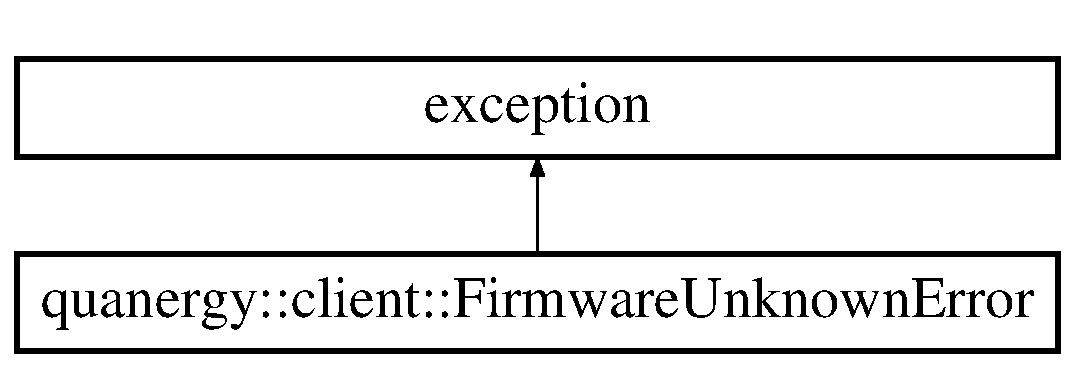
\includegraphics[height=2.000000cm]{structquanergy_1_1client_1_1FirmwareUnknownError}
\end{center}
\end{figure}
\subsection*{Public Member Functions}
\begin{DoxyCompactItemize}
\item 
\hypertarget{structquanergy_1_1client_1_1FirmwareUnknownError_acba47387e1d8c8b87aca0b0a6e95fc04}{virtual const char $\ast$ {\bfseries what} () const   throw ()}\label{structquanergy_1_1client_1_1FirmwareUnknownError_acba47387e1d8c8b87aca0b0a6e95fc04}

\end{DoxyCompactItemize}


\subsection{Detailed Description}
Firmware unknown error Raised for status bits that are not presently assigned. 

The documentation for this struct was generated from the following file\-:\begin{DoxyCompactItemize}
\item 
\hyperlink{exceptions_8h}{exceptions.\-h}\end{DoxyCompactItemize}

\hypertarget{structquanergy_1_1client_1_1FirmwareVersionMismatchError}{\section{quanergy\-:\-:client\-:\-:Firmware\-Version\-Mismatch\-Error Struct Reference}
\label{structquanergy_1_1client_1_1FirmwareVersionMismatchError}\index{quanergy\-::client\-::\-Firmware\-Version\-Mismatch\-Error@{quanergy\-::client\-::\-Firmware\-Version\-Mismatch\-Error}}
}


Firmware versions on sensor don't match.  




{\ttfamily \#include $<$exceptions.\-h$>$}

Inheritance diagram for quanergy\-:\-:client\-:\-:Firmware\-Version\-Mismatch\-Error\-:\begin{figure}[H]
\begin{center}
\leavevmode
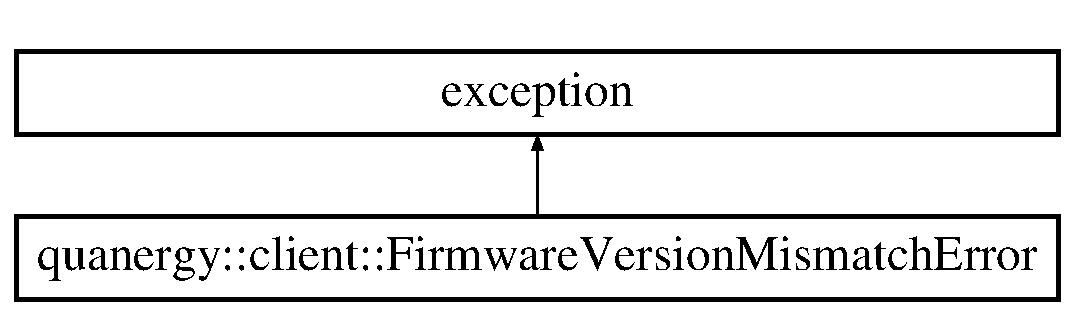
\includegraphics[height=2.000000cm]{structquanergy_1_1client_1_1FirmwareVersionMismatchError}
\end{center}
\end{figure}
\subsection*{Public Member Functions}
\begin{DoxyCompactItemize}
\item 
\hypertarget{structquanergy_1_1client_1_1FirmwareVersionMismatchError_a521b7c22b272973a0f51de6e98e9951d}{virtual const char $\ast$ {\bfseries what} () const   throw ()}\label{structquanergy_1_1client_1_1FirmwareVersionMismatchError_a521b7c22b272973a0f51de6e98e9951d}

\end{DoxyCompactItemize}


\subsection{Detailed Description}
Firmware versions on sensor don't match. 

The documentation for this struct was generated from the following file\-:\begin{DoxyCompactItemize}
\item 
\hyperlink{exceptions_8h}{exceptions.\-h}\end{DoxyCompactItemize}

\hypertarget{structquanergy_1_1client_1_1FirmwareWatchdogViolationError}{\section{quanergy\-:\-:client\-:\-:Firmware\-Watchdog\-Violation\-Error Struct Reference}
\label{structquanergy_1_1client_1_1FirmwareWatchdogViolationError}\index{quanergy\-::client\-::\-Firmware\-Watchdog\-Violation\-Error@{quanergy\-::client\-::\-Firmware\-Watchdog\-Violation\-Error}}
}


Firmware watchdog is not receiving an internal signal.  




{\ttfamily \#include $<$exceptions.\-h$>$}

Inheritance diagram for quanergy\-:\-:client\-:\-:Firmware\-Watchdog\-Violation\-Error\-:\begin{figure}[H]
\begin{center}
\leavevmode
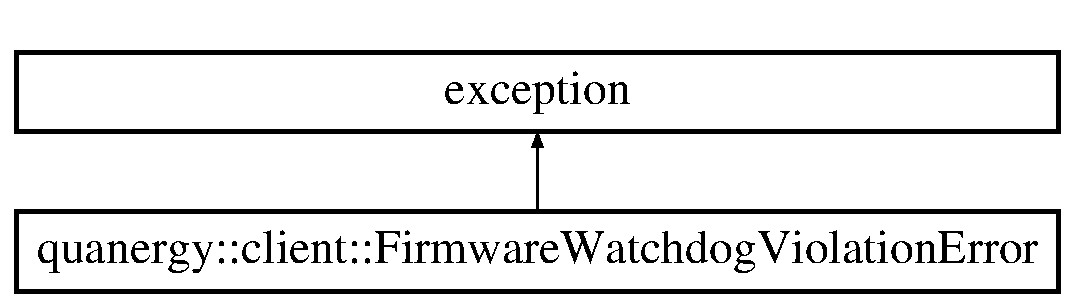
\includegraphics[height=2.000000cm]{structquanergy_1_1client_1_1FirmwareWatchdogViolationError}
\end{center}
\end{figure}
\subsection*{Public Member Functions}
\begin{DoxyCompactItemize}
\item 
\hypertarget{structquanergy_1_1client_1_1FirmwareWatchdogViolationError_a840c24c7804eddc85bbe033247b2a447}{virtual const char $\ast$ {\bfseries what} () const   throw ()}\label{structquanergy_1_1client_1_1FirmwareWatchdogViolationError_a840c24c7804eddc85bbe033247b2a447}

\end{DoxyCompactItemize}


\subsection{Detailed Description}
Firmware watchdog is not receiving an internal signal. 

The documentation for this struct was generated from the following file\-:\begin{DoxyCompactItemize}
\item 
\hyperlink{exceptions_8h}{exceptions.\-h}\end{DoxyCompactItemize}

\hypertarget{structquanergy_1_1client_1_1InvalidDataTypeError}{\section{quanergy\-:\-:client\-:\-:Invalid\-Data\-Type\-Error Struct Reference}
\label{structquanergy_1_1client_1_1InvalidDataTypeError}\index{quanergy\-::client\-::\-Invalid\-Data\-Type\-Error@{quanergy\-::client\-::\-Invalid\-Data\-Type\-Error}}
}


Invalid data type in header; no parser available.  




{\ttfamily \#include $<$exceptions.\-h$>$}

Inheritance diagram for quanergy\-:\-:client\-:\-:Invalid\-Data\-Type\-Error\-:\begin{figure}[H]
\begin{center}
\leavevmode
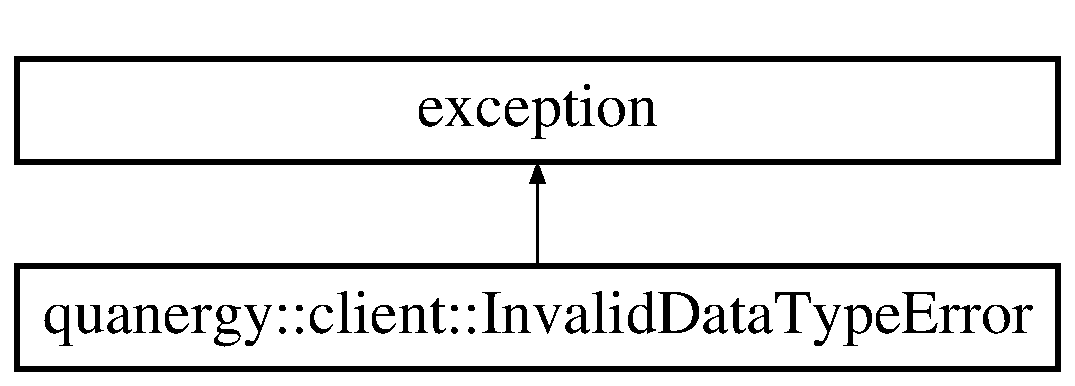
\includegraphics[height=2.000000cm]{structquanergy_1_1client_1_1InvalidDataTypeError}
\end{center}
\end{figure}
\subsection*{Public Member Functions}
\begin{DoxyCompactItemize}
\item 
\hypertarget{structquanergy_1_1client_1_1InvalidDataTypeError_ac0933a83bd02c949f584543a8729a4ac}{virtual const char $\ast$ {\bfseries what} () const   throw ()}\label{structquanergy_1_1client_1_1InvalidDataTypeError_ac0933a83bd02c949f584543a8729a4ac}

\end{DoxyCompactItemize}


\subsection{Detailed Description}
Invalid data type in header; no parser available. 

The documentation for this struct was generated from the following file\-:\begin{DoxyCompactItemize}
\item 
\hyperlink{exceptions_8h}{exceptions.\-h}\end{DoxyCompactItemize}

\hypertarget{structquanergy_1_1client_1_1InvalidDataVersionError}{\section{quanergy\-:\-:client\-:\-:Invalid\-Data\-Version\-Error Struct Reference}
\label{structquanergy_1_1client_1_1InvalidDataVersionError}\index{quanergy\-::client\-::\-Invalid\-Data\-Version\-Error@{quanergy\-::client\-::\-Invalid\-Data\-Version\-Error}}
}


Invalid version for type.  




{\ttfamily \#include $<$exceptions.\-h$>$}

Inheritance diagram for quanergy\-:\-:client\-:\-:Invalid\-Data\-Version\-Error\-:\begin{figure}[H]
\begin{center}
\leavevmode
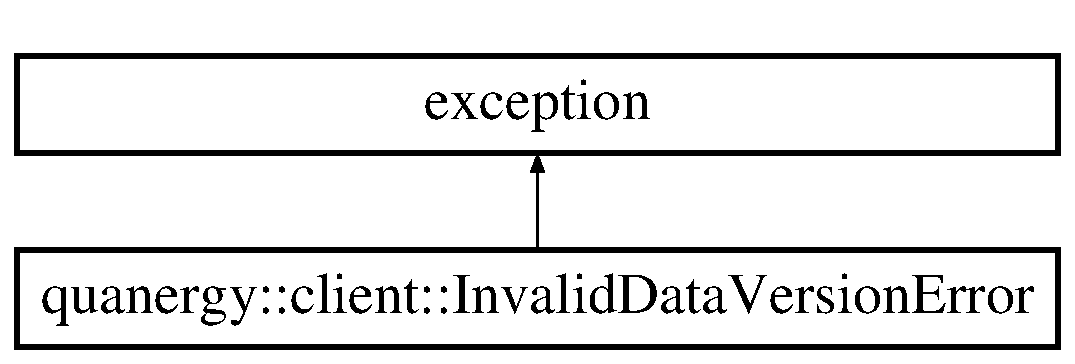
\includegraphics[height=2.000000cm]{structquanergy_1_1client_1_1InvalidDataVersionError}
\end{center}
\end{figure}
\subsection*{Public Member Functions}
\begin{DoxyCompactItemize}
\item 
\hypertarget{structquanergy_1_1client_1_1InvalidDataVersionError_a51a26ca8d5ff1fccf68976886602646a}{virtual const char $\ast$ {\bfseries what} () const   throw ()}\label{structquanergy_1_1client_1_1InvalidDataVersionError_a51a26ca8d5ff1fccf68976886602646a}

\end{DoxyCompactItemize}


\subsection{Detailed Description}
Invalid version for type. 

The documentation for this struct was generated from the following file\-:\begin{DoxyCompactItemize}
\item 
\hyperlink{exceptions_8h}{exceptions.\-h}\end{DoxyCompactItemize}

\hypertarget{structquanergy_1_1client_1_1InvalidDegreesPerCloud}{\section{quanergy\-:\-:client\-:\-:Invalid\-Degrees\-Per\-Cloud Struct Reference}
\label{structquanergy_1_1client_1_1InvalidDegreesPerCloud}\index{quanergy\-::client\-::\-Invalid\-Degrees\-Per\-Cloud@{quanergy\-::client\-::\-Invalid\-Degrees\-Per\-Cloud}}
}


Degress per cloud must be 360 or less.  




{\ttfamily \#include $<$exceptions.\-h$>$}

Inheritance diagram for quanergy\-:\-:client\-:\-:Invalid\-Degrees\-Per\-Cloud\-:\begin{figure}[H]
\begin{center}
\leavevmode
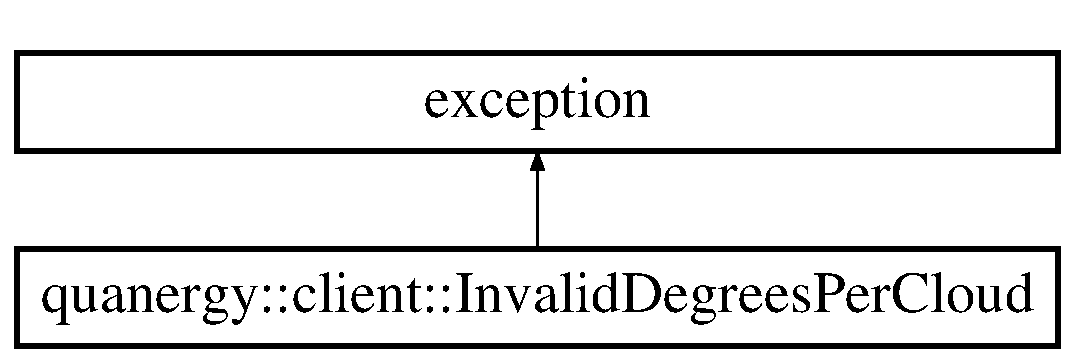
\includegraphics[height=2.000000cm]{structquanergy_1_1client_1_1InvalidDegreesPerCloud}
\end{center}
\end{figure}
\subsection*{Public Member Functions}
\begin{DoxyCompactItemize}
\item 
\hypertarget{structquanergy_1_1client_1_1InvalidDegreesPerCloud_abdf086dd2a96974a830c9b8b45c11a4f}{virtual const char $\ast$ {\bfseries what} () const   throw ()}\label{structquanergy_1_1client_1_1InvalidDegreesPerCloud_abdf086dd2a96974a830c9b8b45c11a4f}

\end{DoxyCompactItemize}


\subsection{Detailed Description}
Degress per cloud must be 360 or less. 

The documentation for this struct was generated from the following file\-:\begin{DoxyCompactItemize}
\item 
\hyperlink{exceptions_8h}{exceptions.\-h}\end{DoxyCompactItemize}

\hypertarget{structquanergy_1_1client_1_1InvalidHeaderError}{\section{quanergy\-:\-:client\-:\-:Invalid\-Header\-Error Struct Reference}
\label{structquanergy_1_1client_1_1InvalidHeaderError}\index{quanergy\-::client\-::\-Invalid\-Header\-Error@{quanergy\-::client\-::\-Invalid\-Header\-Error}}
}


error parsing header  




{\ttfamily \#include $<$exceptions.\-h$>$}

Inheritance diagram for quanergy\-:\-:client\-:\-:Invalid\-Header\-Error\-:\begin{figure}[H]
\begin{center}
\leavevmode
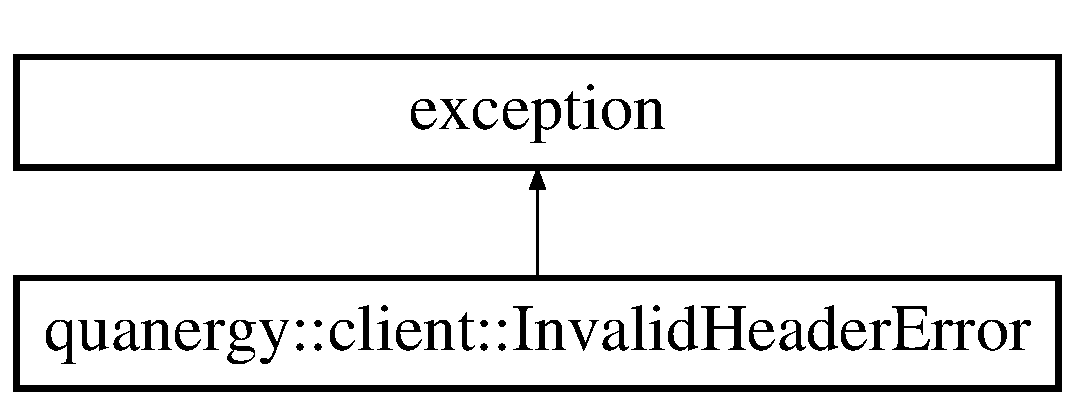
\includegraphics[height=2.000000cm]{structquanergy_1_1client_1_1InvalidHeaderError}
\end{center}
\end{figure}
\subsection*{Public Member Functions}
\begin{DoxyCompactItemize}
\item 
\hypertarget{structquanergy_1_1client_1_1InvalidHeaderError_a3e7c2a648f3e6b23556fe667407b0e4f}{virtual const char $\ast$ {\bfseries what} () const   throw ()}\label{structquanergy_1_1client_1_1InvalidHeaderError_a3e7c2a648f3e6b23556fe667407b0e4f}

\end{DoxyCompactItemize}


\subsection{Detailed Description}
error parsing header 

The documentation for this struct was generated from the following file\-:\begin{DoxyCompactItemize}
\item 
\hyperlink{exceptions_8h}{exceptions.\-h}\end{DoxyCompactItemize}

\hypertarget{structquanergy_1_1client_1_1InvalidPacketError}{\section{quanergy\-:\-:client\-:\-:Invalid\-Packet\-Error Struct Reference}
\label{structquanergy_1_1client_1_1InvalidPacketError}\index{quanergy\-::client\-::\-Invalid\-Packet\-Error@{quanergy\-::client\-::\-Invalid\-Packet\-Error}}
}


Invalid packet.  




{\ttfamily \#include $<$exceptions.\-h$>$}

Inheritance diagram for quanergy\-:\-:client\-:\-:Invalid\-Packet\-Error\-:\begin{figure}[H]
\begin{center}
\leavevmode
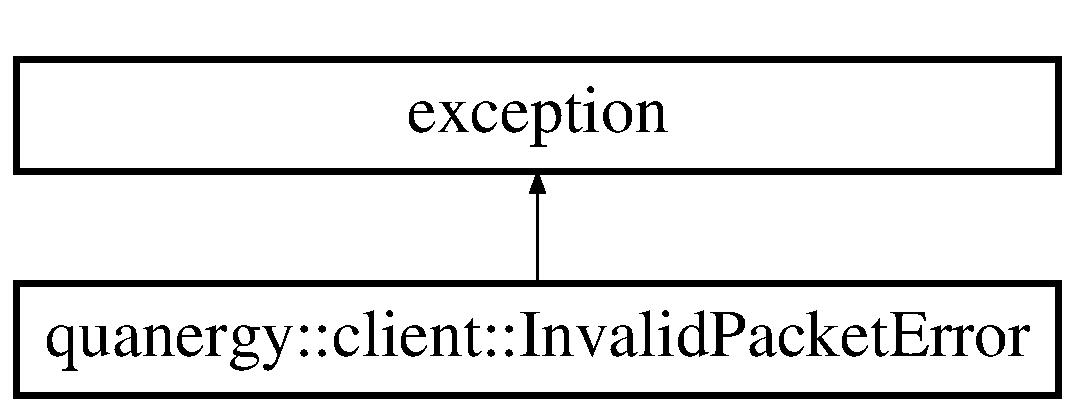
\includegraphics[height=2.000000cm]{structquanergy_1_1client_1_1InvalidPacketError}
\end{center}
\end{figure}
\subsection*{Public Member Functions}
\begin{DoxyCompactItemize}
\item 
\hypertarget{structquanergy_1_1client_1_1InvalidPacketError_a6fd9a698e1217fd84ab1eb0c44d46648}{virtual const char $\ast$ {\bfseries what} () const   throw ()}\label{structquanergy_1_1client_1_1InvalidPacketError_a6fd9a698e1217fd84ab1eb0c44d46648}

\end{DoxyCompactItemize}


\subsection{Detailed Description}
Invalid packet. 

The documentation for this struct was generated from the following file\-:\begin{DoxyCompactItemize}
\item 
\hyperlink{exceptions_8h}{exceptions.\-h}\end{DoxyCompactItemize}

\hypertarget{structquanergy_1_1client_1_1InvalidReturnSelection}{\section{quanergy\-:\-:client\-:\-:Invalid\-Return\-Selection Struct Reference}
\label{structquanergy_1_1client_1_1InvalidReturnSelection}\index{quanergy\-::client\-::\-Invalid\-Return\-Selection@{quanergy\-::client\-::\-Invalid\-Return\-Selection}}
}


Return selction must be less than M8\-\_\-\-N\-U\-M\-\_\-\-R\-E\-T\-U\-R\-N\-S.  




{\ttfamily \#include $<$exceptions.\-h$>$}

Inheritance diagram for quanergy\-:\-:client\-:\-:Invalid\-Return\-Selection\-:\begin{figure}[H]
\begin{center}
\leavevmode
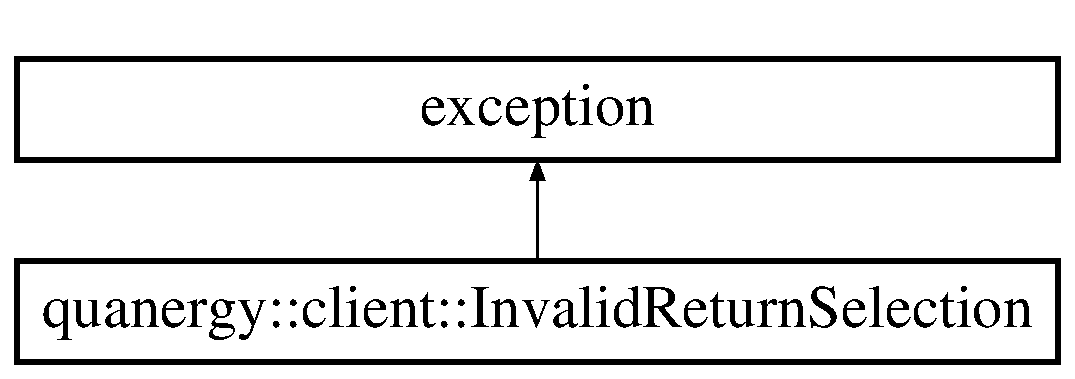
\includegraphics[height=2.000000cm]{structquanergy_1_1client_1_1InvalidReturnSelection}
\end{center}
\end{figure}
\subsection*{Public Member Functions}
\begin{DoxyCompactItemize}
\item 
\hypertarget{structquanergy_1_1client_1_1InvalidReturnSelection_a7e00dadd733995353275c23db2805829}{virtual const char $\ast$ {\bfseries what} () const   throw ()}\label{structquanergy_1_1client_1_1InvalidReturnSelection_a7e00dadd733995353275c23db2805829}

\end{DoxyCompactItemize}


\subsection{Detailed Description}
Return selction must be less than M8\-\_\-\-N\-U\-M\-\_\-\-R\-E\-T\-U\-R\-N\-S. 

The documentation for this struct was generated from the following file\-:\begin{DoxyCompactItemize}
\item 
\hyperlink{exceptions_8h}{exceptions.\-h}\end{DoxyCompactItemize}

\hypertarget{structquanergy_1_1client_1_1M8DataPacket}{\section{quanergy\-:\-:client\-:\-:M8\-Data\-Packet Struct Reference}
\label{structquanergy_1_1client_1_1M8DataPacket}\index{quanergy\-::client\-::\-M8\-Data\-Packet@{quanergy\-::client\-::\-M8\-Data\-Packet}}
}


structure that holds multiple sensor firings and gets sent in the T\-C\-P packet  




{\ttfamily \#include $<$m8\-\_\-data\-\_\-packet.\-h$>$}

\subsection*{Public Attributes}
\begin{DoxyCompactItemize}
\item 
\hypertarget{structquanergy_1_1client_1_1M8DataPacket_aef4dc4c367369ce9c6bfe6f113339f28}{\hyperlink{structquanergy_1_1client_1_1M8FiringData}{M8\-Firing\-Data} {\bfseries data} \mbox{[}M8\-\_\-\-F\-I\-R\-I\-N\-G\-\_\-\-P\-E\-R\-\_\-\-P\-K\-T\mbox{]}}\label{structquanergy_1_1client_1_1M8DataPacket_aef4dc4c367369ce9c6bfe6f113339f28}

\item 
\hypertarget{structquanergy_1_1client_1_1M8DataPacket_a0d786879e71494b8b8151a567ab4460d}{std\-::uint32\-\_\-t {\bfseries seconds}}\label{structquanergy_1_1client_1_1M8DataPacket_a0d786879e71494b8b8151a567ab4460d}

\item 
\hypertarget{structquanergy_1_1client_1_1M8DataPacket_a9ecaa99ba83ffb647788d90f913fb6c7}{std\-::uint32\-\_\-t {\bfseries nanoseconds}}\label{structquanergy_1_1client_1_1M8DataPacket_a9ecaa99ba83ffb647788d90f913fb6c7}

\item 
\hypertarget{structquanergy_1_1client_1_1M8DataPacket_a11378e45d412431268b093e4b343588f}{std\-::uint16\-\_\-t {\bfseries version}}\label{structquanergy_1_1client_1_1M8DataPacket_a11378e45d412431268b093e4b343588f}

\item 
\hypertarget{structquanergy_1_1client_1_1M8DataPacket_a611cc8752437f8c491d5a60e06dac6cb}{std\-::uint16\-\_\-t {\bfseries status}}\label{structquanergy_1_1client_1_1M8DataPacket_a611cc8752437f8c491d5a60e06dac6cb}

\end{DoxyCompactItemize}


\subsection{Detailed Description}
structure that holds multiple sensor firings and gets sent in the T\-C\-P packet 

The documentation for this struct was generated from the following file\-:\begin{DoxyCompactItemize}
\item 
\hyperlink{m8__data__packet_8h}{m8\-\_\-data\-\_\-packet.\-h}\end{DoxyCompactItemize}

\hypertarget{structquanergy_1_1client_1_1M8DataPacket04}{\section{quanergy\-:\-:client\-:\-:M8\-Data\-Packet04 Struct Reference}
\label{structquanergy_1_1client_1_1M8DataPacket04}\index{quanergy\-::client\-::\-M8\-Data\-Packet04@{quanergy\-::client\-::\-M8\-Data\-Packet04}}
}
\subsection*{Public Attributes}
\begin{DoxyCompactItemize}
\item 
\hypertarget{structquanergy_1_1client_1_1M8DataPacket04_afc73b943d01a6ad7cc4445ddb6c5d65a}{\hyperlink{structquanergy_1_1client_1_1M8DataPacket04Header}{M8\-Data\-Packet04\-Header} {\bfseries data\-\_\-header}}\label{structquanergy_1_1client_1_1M8DataPacket04_afc73b943d01a6ad7cc4445ddb6c5d65a}

\item 
\hypertarget{structquanergy_1_1client_1_1M8DataPacket04_ab816133b5ada68f42df5a5b895080ddb}{\hyperlink{structquanergy_1_1client_1_1M8FiringData04}{M8\-Firing\-Data04} {\bfseries firings} \mbox{[}M8\-\_\-\-F\-I\-R\-I\-N\-G\-\_\-\-P\-E\-R\-\_\-\-P\-K\-T\mbox{]}}\label{structquanergy_1_1client_1_1M8DataPacket04_ab816133b5ada68f42df5a5b895080ddb}

\end{DoxyCompactItemize}


The documentation for this struct was generated from the following file\-:\begin{DoxyCompactItemize}
\item 
\hyperlink{data__packet__04_8h}{data\-\_\-packet\-\_\-04.\-h}\end{DoxyCompactItemize}

\hypertarget{structquanergy_1_1client_1_1M8DataPacket04Header}{\section{quanergy\-:\-:client\-:\-:M8\-Data\-Packet04\-Header Struct Reference}
\label{structquanergy_1_1client_1_1M8DataPacket04Header}\index{quanergy\-::client\-::\-M8\-Data\-Packet04\-Header@{quanergy\-::client\-::\-M8\-Data\-Packet04\-Header}}
}
\subsection*{Public Attributes}
\begin{DoxyCompactItemize}
\item 
\hypertarget{structquanergy_1_1client_1_1M8DataPacket04Header_a95367db8adefccee232d7612eb6fc9ba}{std\-::uint16\-\_\-t {\bfseries status}}\label{structquanergy_1_1client_1_1M8DataPacket04Header_a95367db8adefccee232d7612eb6fc9ba}

\item 
\hypertarget{structquanergy_1_1client_1_1M8DataPacket04Header_a3b04a8ab4cd2c30b07ac878f4360cedb}{std\-::uint8\-\_\-t {\bfseries return\-\_\-id}}\label{structquanergy_1_1client_1_1M8DataPacket04Header_a3b04a8ab4cd2c30b07ac878f4360cedb}

\item 
\hypertarget{structquanergy_1_1client_1_1M8DataPacket04Header_a384ed28e289a1cbbb295626f52aab874}{std\-::uint8\-\_\-t {\bfseries reserved}}\label{structquanergy_1_1client_1_1M8DataPacket04Header_a384ed28e289a1cbbb295626f52aab874}

\end{DoxyCompactItemize}


The documentation for this struct was generated from the following file\-:\begin{DoxyCompactItemize}
\item 
\hyperlink{data__packet__04_8h}{data\-\_\-packet\-\_\-04.\-h}\end{DoxyCompactItemize}

\hypertarget{structquanergy_1_1client_1_1M8FiringData}{\section{quanergy\-:\-:client\-:\-:M8\-Firing\-Data Struct Reference}
\label{structquanergy_1_1client_1_1M8FiringData}\index{quanergy\-::client\-::\-M8\-Firing\-Data@{quanergy\-::client\-::\-M8\-Firing\-Data}}
}


structure that holds the sensor firing output  




{\ttfamily \#include $<$m8\-\_\-data\-\_\-packet.\-h$>$}

\subsection*{Public Attributes}
\begin{DoxyCompactItemize}
\item 
\hypertarget{structquanergy_1_1client_1_1M8FiringData_a66d58644fd2aa753754ed3e185f2c6ca}{std\-::uint16\-\_\-t {\bfseries position}}\label{structquanergy_1_1client_1_1M8FiringData_a66d58644fd2aa753754ed3e185f2c6ca}

\item 
\hypertarget{structquanergy_1_1client_1_1M8FiringData_a94b53903975e9b9bee5f9e017cb65fba}{std\-::uint16\-\_\-t {\bfseries padding}}\label{structquanergy_1_1client_1_1M8FiringData_a94b53903975e9b9bee5f9e017cb65fba}

\item 
\hypertarget{structquanergy_1_1client_1_1M8FiringData_a435104d84db4af5f9876942ccecbab36}{std\-::uint32\-\_\-t {\bfseries returns\-\_\-distances} \mbox{[}M8\-\_\-\-N\-U\-M\-\_\-\-R\-E\-T\-U\-R\-N\-S\mbox{]}\mbox{[}M8\-\_\-\-N\-U\-M\-\_\-\-L\-A\-S\-E\-R\-S\mbox{]}}\label{structquanergy_1_1client_1_1M8FiringData_a435104d84db4af5f9876942ccecbab36}

\item 
\hypertarget{structquanergy_1_1client_1_1M8FiringData_aff116b9e02ac6d14b2e401fcfcbce0b0}{std\-::uint8\-\_\-t {\bfseries returns\-\_\-intensities} \mbox{[}M8\-\_\-\-N\-U\-M\-\_\-\-R\-E\-T\-U\-R\-N\-S\mbox{]}\mbox{[}M8\-\_\-\-N\-U\-M\-\_\-\-L\-A\-S\-E\-R\-S\mbox{]}}\label{structquanergy_1_1client_1_1M8FiringData_aff116b9e02ac6d14b2e401fcfcbce0b0}

\item 
\hypertarget{structquanergy_1_1client_1_1M8FiringData_ab1f016a109b4a8121e04c6c886ceaa07}{std\-::uint8\-\_\-t {\bfseries returns\-\_\-status} \mbox{[}M8\-\_\-\-N\-U\-M\-\_\-\-L\-A\-S\-E\-R\-S\mbox{]}}\label{structquanergy_1_1client_1_1M8FiringData_ab1f016a109b4a8121e04c6c886ceaa07}

\end{DoxyCompactItemize}


\subsection{Detailed Description}
structure that holds the sensor firing output 

The documentation for this struct was generated from the following file\-:\begin{DoxyCompactItemize}
\item 
\hyperlink{m8__data__packet_8h}{m8\-\_\-data\-\_\-packet.\-h}\end{DoxyCompactItemize}

\hypertarget{structquanergy_1_1client_1_1M8FiringData04}{\section{quanergy\-:\-:client\-:\-:M8\-Firing\-Data04 Struct Reference}
\label{structquanergy_1_1client_1_1M8FiringData04}\index{quanergy\-::client\-::\-M8\-Firing\-Data04@{quanergy\-::client\-::\-M8\-Firing\-Data04}}
}
\subsection*{Public Attributes}
\begin{DoxyCompactItemize}
\item 
\hypertarget{structquanergy_1_1client_1_1M8FiringData04_a1af27702635007a368cd8c1be0ab755a}{std\-::uint16\-\_\-t {\bfseries position}}\label{structquanergy_1_1client_1_1M8FiringData04_a1af27702635007a368cd8c1be0ab755a}

\item 
\hypertarget{structquanergy_1_1client_1_1M8FiringData04_afa51d6d14df19877acbfe95cfdba6ca7}{std\-::uint16\-\_\-t {\bfseries reserved}}\label{structquanergy_1_1client_1_1M8FiringData04_afa51d6d14df19877acbfe95cfdba6ca7}

\item 
\hypertarget{structquanergy_1_1client_1_1M8FiringData04_ade428aa1f8c3a5ff5547b35ce3fc2d82}{std\-::uint32\-\_\-t {\bfseries radius} \mbox{[}M8\-\_\-\-N\-U\-M\-\_\-\-L\-A\-S\-E\-R\-S\mbox{]}}\label{structquanergy_1_1client_1_1M8FiringData04_ade428aa1f8c3a5ff5547b35ce3fc2d82}

\item 
\hypertarget{structquanergy_1_1client_1_1M8FiringData04_a889d0abf171b7b7c2df43a42a945a0f4}{std\-::uint8\-\_\-t {\bfseries intensity} \mbox{[}M8\-\_\-\-N\-U\-M\-\_\-\-L\-A\-S\-E\-R\-S\mbox{]}}\label{structquanergy_1_1client_1_1M8FiringData04_a889d0abf171b7b7c2df43a42a945a0f4}

\end{DoxyCompactItemize}


The documentation for this struct was generated from the following file\-:\begin{DoxyCompactItemize}
\item 
\hyperlink{data__packet__04_8h}{data\-\_\-packet\-\_\-04.\-h}\end{DoxyCompactItemize}

\hypertarget{structquanergy_1_1client_1_1PacketHeader}{\section{quanergy\-:\-:client\-:\-:Packet\-Header Struct Reference}
\label{structquanergy_1_1client_1_1PacketHeader}\index{quanergy\-::client\-::\-Packet\-Header@{quanergy\-::client\-::\-Packet\-Header}}
}


Header shared by all messages.  




{\ttfamily \#include $<$packet\-\_\-header.\-h$>$}

\subsection*{Public Attributes}
\begin{DoxyCompactItemize}
\item 
\hypertarget{structquanergy_1_1client_1_1PacketHeader_a0113ae6ee537998b0d5357f3768fa51d}{std\-::uint32\-\_\-t {\bfseries signature}}\label{structquanergy_1_1client_1_1PacketHeader_a0113ae6ee537998b0d5357f3768fa51d}

\item 
\hypertarget{structquanergy_1_1client_1_1PacketHeader_a6d20d42b68991dee912d107855eb9617}{std\-::uint32\-\_\-t {\bfseries size}}\label{structquanergy_1_1client_1_1PacketHeader_a6d20d42b68991dee912d107855eb9617}

\item 
\hypertarget{structquanergy_1_1client_1_1PacketHeader_aa6b56fb5edde8906b255a6bf087fc961}{std\-::uint32\-\_\-t {\bfseries seconds}}\label{structquanergy_1_1client_1_1PacketHeader_aa6b56fb5edde8906b255a6bf087fc961}

\item 
\hypertarget{structquanergy_1_1client_1_1PacketHeader_aec03a337cba2b481b082015fbc2f75f8}{std\-::uint32\-\_\-t {\bfseries nanoseconds}}\label{structquanergy_1_1client_1_1PacketHeader_aec03a337cba2b481b082015fbc2f75f8}

\item 
\hypertarget{structquanergy_1_1client_1_1PacketHeader_ac36cd21bcc2ccd8388e1db2b8585f7a9}{std\-::uint8\-\_\-t {\bfseries version\-\_\-major}}\label{structquanergy_1_1client_1_1PacketHeader_ac36cd21bcc2ccd8388e1db2b8585f7a9}

\item 
\hypertarget{structquanergy_1_1client_1_1PacketHeader_ac8bcd8965a90bbf5312f21c7d310ecad}{std\-::uint8\-\_\-t {\bfseries version\-\_\-minor}}\label{structquanergy_1_1client_1_1PacketHeader_ac8bcd8965a90bbf5312f21c7d310ecad}

\item 
\hypertarget{structquanergy_1_1client_1_1PacketHeader_a64f138d48e9fcb2a9f03947cbb40e3f3}{std\-::uint8\-\_\-t {\bfseries version\-\_\-patch}}\label{structquanergy_1_1client_1_1PacketHeader_a64f138d48e9fcb2a9f03947cbb40e3f3}

\item 
\hypertarget{structquanergy_1_1client_1_1PacketHeader_aed77a534a21367441435c794c6adb868}{std\-::uint8\-\_\-t {\bfseries packet\-\_\-type}}\label{structquanergy_1_1client_1_1PacketHeader_aed77a534a21367441435c794c6adb868}

\end{DoxyCompactItemize}


\subsection{Detailed Description}
Header shared by all messages. 

The documentation for this struct was generated from the following file\-:\begin{DoxyCompactItemize}
\item 
packet\-\_\-header.\-h\end{DoxyCompactItemize}

\hypertarget{structquanergy_1_1client_1_1PacketParserBase}{\section{quanergy\-:\-:client\-:\-:Packet\-Parser\-Base$<$ R\-E\-S\-U\-L\-T $>$ Struct Template Reference}
\label{structquanergy_1_1client_1_1PacketParserBase}\index{quanergy\-::client\-::\-Packet\-Parser\-Base$<$ R\-E\-S\-U\-L\-T $>$@{quanergy\-::client\-::\-Packet\-Parser\-Base$<$ R\-E\-S\-U\-L\-T $>$}}
}


base class for packet parsers  




{\ttfamily \#include $<$packet\-\_\-parser.\-h$>$}

Inheritance diagram for quanergy\-:\-:client\-:\-:Packet\-Parser\-Base$<$ R\-E\-S\-U\-L\-T $>$\-:\begin{figure}[H]
\begin{center}
\leavevmode
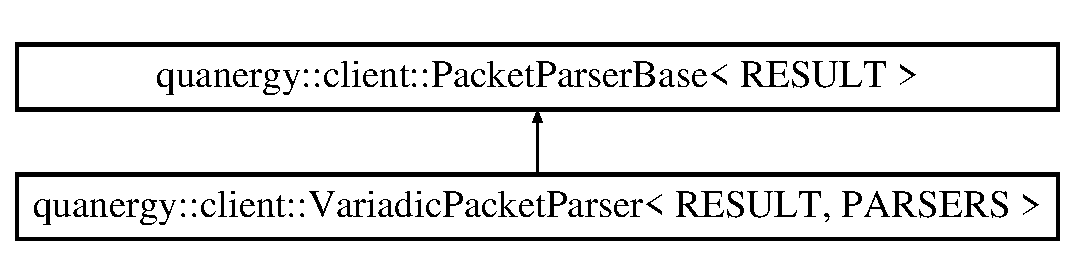
\includegraphics[height=2.000000cm]{structquanergy_1_1client_1_1PacketParserBase}
\end{center}
\end{figure}
\subsection*{Public Member Functions}
\begin{DoxyCompactItemize}
\item 
virtual bool \hyperlink{structquanergy_1_1client_1_1PacketParserBase_ace6f4bff879bd05ec7dbc670802f70c9}{validate\-Parse} (const std\-::vector$<$ char $>$ \&packet, R\-E\-S\-U\-L\-T \&result)
\begin{DoxyCompactList}\small\item\em check packet validity and parse if a match \end{DoxyCompactList}\item 
virtual bool \hyperlink{structquanergy_1_1client_1_1PacketParserBase_ad840fd4e7f3ab054024957ae1d94ffa1}{validate} (const std\-::vector$<$ char $>$ \&packet)=0
\begin{DoxyCompactList}\small\item\em check packet validity \end{DoxyCompactList}\item 
virtual bool \hyperlink{structquanergy_1_1client_1_1PacketParserBase_a4a0555355f550738007edf7994da1c8c}{parse} (const std\-::vector$<$ char $>$ \&packet, R\-E\-S\-U\-L\-T \&result)=0
\begin{DoxyCompactList}\small\item\em parse packet and update result \end{DoxyCompactList}\end{DoxyCompactItemize}


\subsection{Detailed Description}
\subsubsection*{template$<$class R\-E\-S\-U\-L\-T$>$struct quanergy\-::client\-::\-Packet\-Parser\-Base$<$ R\-E\-S\-U\-L\-T $>$}

base class for packet parsers 

\subsection{Member Function Documentation}
\hypertarget{structquanergy_1_1client_1_1PacketParserBase_a4a0555355f550738007edf7994da1c8c}{\index{quanergy\-::client\-::\-Packet\-Parser\-Base@{quanergy\-::client\-::\-Packet\-Parser\-Base}!parse@{parse}}
\index{parse@{parse}!quanergy::client::PacketParserBase@{quanergy\-::client\-::\-Packet\-Parser\-Base}}
\subsubsection[{parse}]{\setlength{\rightskip}{0pt plus 5cm}template$<$class R\-E\-S\-U\-L\-T$>$ virtual bool {\bf quanergy\-::client\-::\-Packet\-Parser\-Base}$<$ R\-E\-S\-U\-L\-T $>$\-::parse (
\begin{DoxyParamCaption}
\item[{const std\-::vector$<$ char $>$ \&}]{packet, }
\item[{R\-E\-S\-U\-L\-T \&}]{result}
\end{DoxyParamCaption}
)\hspace{0.3cm}{\ttfamily [pure virtual]}}}\label{structquanergy_1_1client_1_1PacketParserBase_a4a0555355f550738007edf7994da1c8c}


parse packet and update result 

\begin{DoxyReturn}{Returns}
true if result updated; false otherwise (some parsers may require multiple packets before updating result) 
\end{DoxyReturn}


Implemented in \hyperlink{structquanergy_1_1client_1_1VariadicPacketParser_af66c0c1212314c43f6a183e7a4711e44}{quanergy\-::client\-::\-Variadic\-Packet\-Parser$<$ R\-E\-S\-U\-L\-T, P\-A\-R\-S\-E\-R\-S $>$}, \hyperlink{structquanergy_1_1client_1_1DataPacketParser04_a62df767eabc53340282c4f3cb5fec9e0}{quanergy\-::client\-::\-Data\-Packet\-Parser04}, \hyperlink{structquanergy_1_1client_1_1DataPacketParser00_aceab95c7e5553724883adad72485d080}{quanergy\-::client\-::\-Data\-Packet\-Parser00}, and \hyperlink{structquanergy_1_1client_1_1DataPacketParser01_a5873c64ebd1b6261e6c6ec8694ab0061}{quanergy\-::client\-::\-Data\-Packet\-Parser01}.

\hypertarget{structquanergy_1_1client_1_1PacketParserBase_ad840fd4e7f3ab054024957ae1d94ffa1}{\index{quanergy\-::client\-::\-Packet\-Parser\-Base@{quanergy\-::client\-::\-Packet\-Parser\-Base}!validate@{validate}}
\index{validate@{validate}!quanergy::client::PacketParserBase@{quanergy\-::client\-::\-Packet\-Parser\-Base}}
\subsubsection[{validate}]{\setlength{\rightskip}{0pt plus 5cm}template$<$class R\-E\-S\-U\-L\-T$>$ virtual bool {\bf quanergy\-::client\-::\-Packet\-Parser\-Base}$<$ R\-E\-S\-U\-L\-T $>$\-::validate (
\begin{DoxyParamCaption}
\item[{const std\-::vector$<$ char $>$ \&}]{packet}
\end{DoxyParamCaption}
)\hspace{0.3cm}{\ttfamily [pure virtual]}}}\label{structquanergy_1_1client_1_1PacketParserBase_ad840fd4e7f3ab054024957ae1d94ffa1}


check packet validity 

\begin{DoxyReturn}{Returns}
true if valid, false otherwise 
\end{DoxyReturn}


Implemented in \hyperlink{structquanergy_1_1client_1_1VariadicPacketParser_a5b53284ba762fc0d9355d28f552bd674}{quanergy\-::client\-::\-Variadic\-Packet\-Parser$<$ R\-E\-S\-U\-L\-T, P\-A\-R\-S\-E\-R\-S $>$}, \hyperlink{structquanergy_1_1client_1_1DataPacketParser04_a4f8566ff529171e458ab2139c9098403}{quanergy\-::client\-::\-Data\-Packet\-Parser04}, \hyperlink{structquanergy_1_1client_1_1DataPacketParser00_ac161241641118826d0514d293f7d6538}{quanergy\-::client\-::\-Data\-Packet\-Parser00}, and \hyperlink{structquanergy_1_1client_1_1DataPacketParser01_a0a28a9b2fecdd1cbb0afb8df05e1f90e}{quanergy\-::client\-::\-Data\-Packet\-Parser01}.

\hypertarget{structquanergy_1_1client_1_1PacketParserBase_ace6f4bff879bd05ec7dbc670802f70c9}{\index{quanergy\-::client\-::\-Packet\-Parser\-Base@{quanergy\-::client\-::\-Packet\-Parser\-Base}!validate\-Parse@{validate\-Parse}}
\index{validate\-Parse@{validate\-Parse}!quanergy::client::PacketParserBase@{quanergy\-::client\-::\-Packet\-Parser\-Base}}
\subsubsection[{validate\-Parse}]{\setlength{\rightskip}{0pt plus 5cm}template$<$class R\-E\-S\-U\-L\-T$>$ virtual bool {\bf quanergy\-::client\-::\-Packet\-Parser\-Base}$<$ R\-E\-S\-U\-L\-T $>$\-::validate\-Parse (
\begin{DoxyParamCaption}
\item[{const std\-::vector$<$ char $>$ \&}]{packet, }
\item[{R\-E\-S\-U\-L\-T \&}]{result}
\end{DoxyParamCaption}
)\hspace{0.3cm}{\ttfamily [inline]}, {\ttfamily [virtual]}}}\label{structquanergy_1_1client_1_1PacketParserBase_ace6f4bff879bd05ec7dbc670802f70c9}


check packet validity and parse if a match 

\begin{DoxyReturn}{Returns}
true if result updated; false otherwise 
\end{DoxyReturn}

\begin{DoxyExceptions}{Exceptions}
{\em \hyperlink{structquanergy_1_1client_1_1InvalidPacketError}{Invalid\-Packet\-Error}} & if not a valid packet \\
\hline
\end{DoxyExceptions}


Reimplemented in \hyperlink{structquanergy_1_1client_1_1VariadicPacketParser_a58a6ec899ab3ee7f2fbd92b4d45082eb}{quanergy\-::client\-::\-Variadic\-Packet\-Parser$<$ R\-E\-S\-U\-L\-T, P\-A\-R\-S\-E\-R\-S $>$}.



The documentation for this struct was generated from the following file\-:\begin{DoxyCompactItemize}
\item 
\hyperlink{packet__parser_8h}{packet\-\_\-parser.\-h}\end{DoxyCompactItemize}

\hypertarget{structquanergy_1_1client_1_1PacketParserModule}{\section{quanergy\-:\-:client\-:\-:Packet\-Parser\-Module$<$ P\-A\-R\-S\-E\-R $>$ Struct Template Reference}
\label{structquanergy_1_1client_1_1PacketParserModule}\index{quanergy\-::client\-::\-Packet\-Parser\-Module$<$ P\-A\-R\-S\-E\-R $>$@{quanergy\-::client\-::\-Packet\-Parser\-Module$<$ P\-A\-R\-S\-E\-R $>$}}
}
Inheritance diagram for quanergy\-:\-:client\-:\-:Packet\-Parser\-Module$<$ P\-A\-R\-S\-E\-R $>$\-:\begin{figure}[H]
\begin{center}
\leavevmode
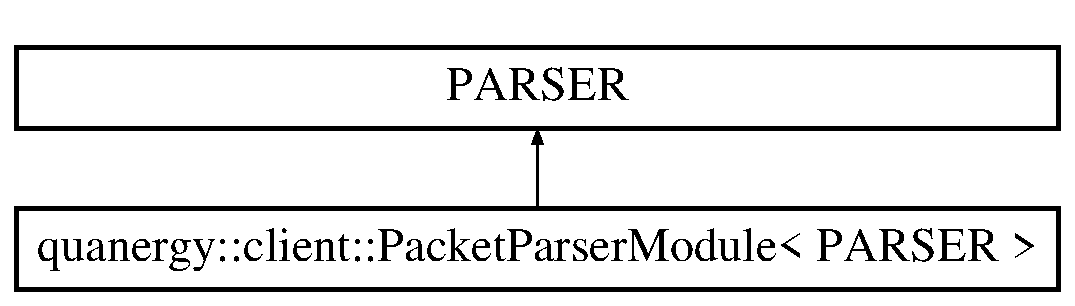
\includegraphics[height=2.000000cm]{structquanergy_1_1client_1_1PacketParserModule}
\end{center}
\end{figure}
\subsection*{Public Types}
\begin{DoxyCompactItemize}
\item 
\hypertarget{structquanergy_1_1client_1_1PacketParserModule_a27105b55007e3ff6713d7775dbac2b6e}{typedef \\*
boost\-::signals2\-::signal$<$ void(const \\*
typename P\-A\-R\-S\-E\-R\-::\-Result\-Type \&)$>$ \hyperlink{structquanergy_1_1client_1_1PacketParserModule_a27105b55007e3ff6713d7775dbac2b6e}{Signal}}\label{structquanergy_1_1client_1_1PacketParserModule_a27105b55007e3ff6713d7775dbac2b6e}

\begin{DoxyCompactList}\small\item\em signal type \end{DoxyCompactList}\end{DoxyCompactItemize}
\subsection*{Public Member Functions}
\begin{DoxyCompactItemize}
\item 
\hypertarget{structquanergy_1_1client_1_1PacketParserModule_aef1a64e8ab6d3eb3aaf79041794d2137}{boost\-::signals2\-::connection \hyperlink{structquanergy_1_1client_1_1PacketParserModule_aef1a64e8ab6d3eb3aaf79041794d2137}{connect} (const typename Signal\-::slot\-\_\-type \&subscriber)}\label{structquanergy_1_1client_1_1PacketParserModule_aef1a64e8ab6d3eb3aaf79041794d2137}

\begin{DoxyCompactList}\small\item\em Connect a slot to the signal which will be emitted when a new R\-E\-S\-U\-L\-T is available. \end{DoxyCompactList}\item 
\hypertarget{structquanergy_1_1client_1_1PacketParserModule_aec3b3652906e440cc226b7091e6e79d3}{void {\bfseries slot} (const std\-::shared\-\_\-ptr$<$ std\-::vector$<$ char $>$$>$ \&packet)}\label{structquanergy_1_1client_1_1PacketParserModule_aec3b3652906e440cc226b7091e6e79d3}

\end{DoxyCompactItemize}
\subsection*{Protected Attributes}
\begin{DoxyCompactItemize}
\item 
\hypertarget{structquanergy_1_1client_1_1PacketParserModule_a690ab0f8b14f9205750c634bdfb62c9c}{\hyperlink{structquanergy_1_1client_1_1PacketParserModule_a27105b55007e3ff6713d7775dbac2b6e}{Signal} \hyperlink{structquanergy_1_1client_1_1PacketParserModule_a690ab0f8b14f9205750c634bdfb62c9c}{signal\-\_\-}}\label{structquanergy_1_1client_1_1PacketParserModule_a690ab0f8b14f9205750c634bdfb62c9c}

\begin{DoxyCompactList}\small\item\em Signal that gets fired whenever a result is ready. \end{DoxyCompactList}\item 
\hypertarget{structquanergy_1_1client_1_1PacketParserModule_adaf4a0cf800ff5c48c79ff865c442f8e}{P\-A\-R\-S\-E\-R\-::\-Result\-Type \hyperlink{structquanergy_1_1client_1_1PacketParserModule_adaf4a0cf800ff5c48c79ff865c442f8e}{result}}\label{structquanergy_1_1client_1_1PacketParserModule_adaf4a0cf800ff5c48c79ff865c442f8e}

\begin{DoxyCompactList}\small\item\em result to pass to parse function \end{DoxyCompactList}\end{DoxyCompactItemize}


The documentation for this struct was generated from the following file\-:\begin{DoxyCompactItemize}
\item 
\hyperlink{packet__parser_8h}{packet\-\_\-parser.\-h}\end{DoxyCompactItemize}

\hypertarget{structquanergy_1_1PointHVDIR}{\section{quanergy\-:\-:Point\-H\-V\-D\-I\-R Struct Reference}
\label{structquanergy_1_1PointHVDIR}\index{quanergy\-::\-Point\-H\-V\-D\-I\-R@{quanergy\-::\-Point\-H\-V\-D\-I\-R}}
}


{\ttfamily \#include $<$point\-\_\-hvdir.\-h$>$}

\subsection*{Public Attributes}
\begin{DoxyCompactItemize}
\item 
\hypertarget{structquanergy_1_1PointHVDIR_a9a31534d462255e0d11a8838c5ea89fa}{{\bfseries P\-C\-L\-\_\-\-A\-D\-D\-\_\-\-P\-O\-I\-N\-T4\-D\-\_\-\-H\-V\-D}}\label{structquanergy_1_1PointHVDIR_a9a31534d462255e0d11a8838c5ea89fa}

\item 
\hypertarget{structquanergy_1_1PointHVDIR_a0fed792362bcfdd4bf79e91b7ab872f2}{float \hyperlink{structquanergy_1_1PointHVDIR_a0fed792362bcfdd4bf79e91b7ab872f2}{intensity}}\label{structquanergy_1_1PointHVDIR_a0fed792362bcfdd4bf79e91b7ab872f2}

\begin{DoxyCompactList}\small\item\em laser intensity reading \end{DoxyCompactList}\item 
\hypertarget{structquanergy_1_1PointHVDIR_a67e32c361914ce014f6d1c081b1596a0}{uint16\-\_\-t \hyperlink{structquanergy_1_1PointHVDIR_a67e32c361914ce014f6d1c081b1596a0}{ring}}\label{structquanergy_1_1PointHVDIR_a67e32c361914ce014f6d1c081b1596a0}

\begin{DoxyCompactList}\small\item\em laser ring number \end{DoxyCompactList}\end{DoxyCompactItemize}


\subsection{Detailed Description}
Polar coordinate, including intensity and ring number. 

The documentation for this struct was generated from the following file\-:\begin{DoxyCompactItemize}
\item 
\hyperlink{point__hvdir_8h}{point\-\_\-hvdir.\-h}\end{DoxyCompactItemize}

\hypertarget{structquanergy_1_1PointXYZ}{\section{quanergy\-:\-:Point\-X\-Y\-Z Struct Reference}
\label{structquanergy_1_1PointXYZ}\index{quanergy\-::\-Point\-X\-Y\-Z@{quanergy\-::\-Point\-X\-Y\-Z}}
}
\subsection*{Public Member Functions}
\begin{DoxyCompactItemize}
\item 
\hypertarget{structquanergy_1_1PointXYZ_a66dc064b33f4ddddec22feda217d0606}{{\bfseries Point\-X\-Y\-Z} (const \hyperlink{structquanergy_1_1PointXYZ}{Point\-X\-Y\-Z} \&p)}\label{structquanergy_1_1PointXYZ_a66dc064b33f4ddddec22feda217d0606}

\item 
\hypertarget{structquanergy_1_1PointXYZ_af9c1f7a49d10418a180452f0ebfbf9fa}{{\bfseries Point\-X\-Y\-Z} (float \-\_\-x, float \-\_\-y, float \-\_\-z)}\label{structquanergy_1_1PointXYZ_af9c1f7a49d10418a180452f0ebfbf9fa}

\item 
\hypertarget{structquanergy_1_1PointXYZ_aa886f6bc333e85307def00cf6f2781d1}{float const \& {\bfseries operator\mbox{[}$\,$\mbox{]}} (std\-::size\-\_\-t index) const }\label{structquanergy_1_1PointXYZ_aa886f6bc333e85307def00cf6f2781d1}

\item 
\hypertarget{structquanergy_1_1PointXYZ_a799b1cf78698e4127fe2b449b5e38901}{float \& {\bfseries operator\mbox{[}$\,$\mbox{]}} (std\-::size\-\_\-t index)}\label{structquanergy_1_1PointXYZ_a799b1cf78698e4127fe2b449b5e38901}

\item 
\hypertarget{structquanergy_1_1PointXYZ_ac36f4072a6cff855cf4ec56d1a1d5314}{{\bfseries operator Eigen\-::\-Vector3f} ()}\label{structquanergy_1_1PointXYZ_ac36f4072a6cff855cf4ec56d1a1d5314}

\end{DoxyCompactItemize}
\subsection*{Public Attributes}
\begin{DoxyCompactItemize}
\item 
\hypertarget{structquanergy_1_1PointXYZ_a05f1335cc8583558284b700c1eecd808}{{\bfseries P\-C\-L\-\_\-\-A\-D\-D\-\_\-\-P\-O\-I\-N\-T4\-D}}\label{structquanergy_1_1PointXYZ_a05f1335cc8583558284b700c1eecd808}

\end{DoxyCompactItemize}
\subsection*{Friends}
\begin{DoxyCompactItemize}
\item 
\hypertarget{structquanergy_1_1PointXYZ_a730340bef93611db89eb2756273637ae}{std\-::ostream \& {\bfseries operator$<$$<$} (std\-::ostream \&out, const \hyperlink{structquanergy_1_1PointXYZ}{Point\-X\-Y\-Z} \&point)}\label{structquanergy_1_1PointXYZ_a730340bef93611db89eb2756273637ae}

\end{DoxyCompactItemize}


The documentation for this struct was generated from the following file\-:\begin{DoxyCompactItemize}
\item 
\hyperlink{point__xyz_8h}{point\-\_\-xyz.\-h}\end{DoxyCompactItemize}

\hypertarget{structquanergy_1_1PointXYZIR}{\section{quanergy\-:\-:Point\-X\-Y\-Z\-I\-R Struct Reference}
\label{structquanergy_1_1PointXYZIR}\index{quanergy\-::\-Point\-X\-Y\-Z\-I\-R@{quanergy\-::\-Point\-X\-Y\-Z\-I\-R}}
}


{\ttfamily \#include $<$point\-\_\-xyzir.\-h$>$}

\subsection*{Public Member Functions}
\begin{DoxyCompactItemize}
\item 
\hypertarget{structquanergy_1_1PointXYZIR_a68e97c0e5cb30c3cbc37e2d5ff812f92}{{\bfseries Point\-X\-Y\-Z\-I\-R} (const \hyperlink{structquanergy_1_1PointXYZIR}{Point\-X\-Y\-Z\-I\-R} \&p)}\label{structquanergy_1_1PointXYZIR_a68e97c0e5cb30c3cbc37e2d5ff812f92}

\item 
\hypertarget{structquanergy_1_1PointXYZIR_afacccd6a267cac839fb9bbc38b069cd2}{{\bfseries Point\-X\-Y\-Z\-I\-R} (float \-\_\-x, float \-\_\-y, float \-\_\-z, float \-\_\-intensity=0.\-0f, uint16\-\_\-t \-\_\-ring=std\-::numeric\-\_\-limits$<$ uint16\-\_\-t $>$\-::max())}\label{structquanergy_1_1PointXYZIR_afacccd6a267cac839fb9bbc38b069cd2}

\end{DoxyCompactItemize}
\subsection*{Public Attributes}
\begin{DoxyCompactItemize}
\item 
\hypertarget{structquanergy_1_1PointXYZIR_a26be2abe12ae5adf9220940671e62c2b}{{\bfseries P\-C\-L\-\_\-\-A\-D\-D\-\_\-\-P\-O\-I\-N\-T4\-D}}\label{structquanergy_1_1PointXYZIR_a26be2abe12ae5adf9220940671e62c2b}

\item 
\hypertarget{structquanergy_1_1PointXYZIR_a964fda4118869ed37f19257431152a82}{float \hyperlink{structquanergy_1_1PointXYZIR_a964fda4118869ed37f19257431152a82}{intensity}}\label{structquanergy_1_1PointXYZIR_a964fda4118869ed37f19257431152a82}

\begin{DoxyCompactList}\small\item\em laser intensity reading \end{DoxyCompactList}\item 
\hypertarget{structquanergy_1_1PointXYZIR_a62b42a446804ce2dd9d4c8167f8b4c9e}{uint16\-\_\-t \hyperlink{structquanergy_1_1PointXYZIR_a62b42a446804ce2dd9d4c8167f8b4c9e}{ring}}\label{structquanergy_1_1PointXYZIR_a62b42a446804ce2dd9d4c8167f8b4c9e}

\begin{DoxyCompactList}\small\item\em laser ring number \end{DoxyCompactList}\end{DoxyCompactItemize}


\subsection{Detailed Description}
Euclidean coordinate, including intensity and ring number. 

The documentation for this struct was generated from the following file\-:\begin{DoxyCompactItemize}
\item 
\hyperlink{point__xyzir_8h}{point\-\_\-xyzir.\-h}\end{DoxyCompactItemize}

\hypertarget{structquanergy_1_1client_1_1PolarToCartConverter}{\section{quanergy\-:\-:client\-:\-:Polar\-To\-Cart\-Converter Struct Reference}
\label{structquanergy_1_1client_1_1PolarToCartConverter}\index{quanergy\-::client\-::\-Polar\-To\-Cart\-Converter@{quanergy\-::client\-::\-Polar\-To\-Cart\-Converter}}
}
\subsection*{Public Types}
\begin{DoxyCompactItemize}
\item 
\hypertarget{structquanergy_1_1client_1_1PolarToCartConverter_ab948183d78b63eda2db0f271f1770a4a}{typedef std\-::shared\-\_\-ptr\\*
$<$ \hyperlink{structquanergy_1_1client_1_1PolarToCartConverter}{Polar\-To\-Cart\-Converter} $>$ {\bfseries Ptr}}\label{structquanergy_1_1client_1_1PolarToCartConverter_ab948183d78b63eda2db0f271f1770a4a}

\item 
\hypertarget{structquanergy_1_1client_1_1PolarToCartConverter_a3b448df71d623646340e0e96fd24aed4}{typedef Point\-Cloud\-X\-Y\-Z\-I\-R\-Ptr {\bfseries Result\-Type}}\label{structquanergy_1_1client_1_1PolarToCartConverter_a3b448df71d623646340e0e96fd24aed4}

\item 
\hypertarget{structquanergy_1_1client_1_1PolarToCartConverter_ab54ab12f4c6d1741abe111dd8aa0c50e}{typedef \\*
boost\-::signals2\-::signal$<$ void(const \\*
Result\-Type \&)$>$ {\bfseries Signal}}\label{structquanergy_1_1client_1_1PolarToCartConverter_ab54ab12f4c6d1741abe111dd8aa0c50e}

\end{DoxyCompactItemize}
\subsection*{Public Member Functions}
\begin{DoxyCompactItemize}
\item 
\hypertarget{structquanergy_1_1client_1_1PolarToCartConverter_a4499d399c420e3170e564033946c507f}{boost\-::signals2\-::connection {\bfseries connect} (const T\-Y\-P\-E\-N\-A\-M\-E Signal\-::slot\-\_\-type \&subscriber)}\label{structquanergy_1_1client_1_1PolarToCartConverter_a4499d399c420e3170e564033946c507f}

\item 
\hypertarget{structquanergy_1_1client_1_1PolarToCartConverter_aab349ed84215a20e776c659e4db7feb5}{void {\bfseries slot} (Point\-Cloud\-H\-V\-D\-I\-R\-Const\-Ptr const \&)}\label{structquanergy_1_1client_1_1PolarToCartConverter_aab349ed84215a20e776c659e4db7feb5}

\end{DoxyCompactItemize}


The documentation for this struct was generated from the following file\-:\begin{DoxyCompactItemize}
\item 
\hyperlink{polar__to__cart__converter_8h}{polar\-\_\-to\-\_\-cart\-\_\-converter.\-h}\end{DoxyCompactItemize}

\hypertarget{structquanergy_1_1client_1_1ReturnIDMismatchError}{\section{quanergy\-:\-:client\-:\-:Return\-I\-D\-Mismatch\-Error Struct Reference}
\label{structquanergy_1_1client_1_1ReturnIDMismatchError}\index{quanergy\-::client\-::\-Return\-I\-D\-Mismatch\-Error@{quanergy\-::client\-::\-Return\-I\-D\-Mismatch\-Error}}
}


Return I\-D coming from sensor doesn't match requested Return I\-D.  




{\ttfamily \#include $<$exceptions.\-h$>$}

Inheritance diagram for quanergy\-:\-:client\-:\-:Return\-I\-D\-Mismatch\-Error\-:\begin{figure}[H]
\begin{center}
\leavevmode
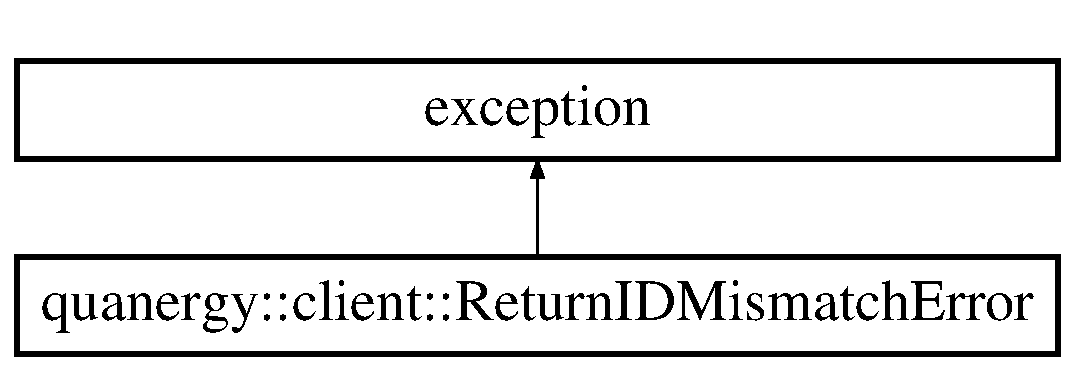
\includegraphics[height=2.000000cm]{structquanergy_1_1client_1_1ReturnIDMismatchError}
\end{center}
\end{figure}
\subsection*{Public Member Functions}
\begin{DoxyCompactItemize}
\item 
\hypertarget{structquanergy_1_1client_1_1ReturnIDMismatchError_a96071210e8a73c35fb54f4fb0d475925}{virtual const char $\ast$ {\bfseries what} () const   throw ()}\label{structquanergy_1_1client_1_1ReturnIDMismatchError_a96071210e8a73c35fb54f4fb0d475925}

\end{DoxyCompactItemize}


\subsection{Detailed Description}
Return I\-D coming from sensor doesn't match requested Return I\-D. 

The documentation for this struct was generated from the following file\-:\begin{DoxyCompactItemize}
\item 
\hyperlink{exceptions_8h}{exceptions.\-h}\end{DoxyCompactItemize}

\hypertarget{structquanergy_1_1client_1_1RingIntensityFilter}{\section{quanergy\-:\-:client\-:\-:Ring\-Intensity\-Filter Struct Reference}
\label{structquanergy_1_1client_1_1RingIntensityFilter}\index{quanergy\-::client\-::\-Ring\-Intensity\-Filter@{quanergy\-::client\-::\-Ring\-Intensity\-Filter}}
}
\subsection*{Public Types}
\begin{DoxyCompactItemize}
\item 
\hypertarget{structquanergy_1_1client_1_1RingIntensityFilter_afa4e8d4876b188636c17907094f54d62}{typedef std\-::shared\-\_\-ptr\\*
$<$ \hyperlink{structquanergy_1_1client_1_1RingIntensityFilter}{Ring\-Intensity\-Filter} $>$ {\bfseries Ptr}}\label{structquanergy_1_1client_1_1RingIntensityFilter_afa4e8d4876b188636c17907094f54d62}

\item 
\hypertarget{structquanergy_1_1client_1_1RingIntensityFilter_a96b133d31719924d92f567ee44056f9e}{typedef Point\-Cloud\-H\-V\-D\-I\-R\-Ptr {\bfseries Result\-Type}}\label{structquanergy_1_1client_1_1RingIntensityFilter_a96b133d31719924d92f567ee44056f9e}

\item 
\hypertarget{structquanergy_1_1client_1_1RingIntensityFilter_a33b71b3190f08792388ac6e37767f247}{typedef \\*
boost\-::signals2\-::signal$<$ void(const \\*
Result\-Type \&)$>$ {\bfseries Signal}}\label{structquanergy_1_1client_1_1RingIntensityFilter_a33b71b3190f08792388ac6e37767f247}

\end{DoxyCompactItemize}
\subsection*{Public Member Functions}
\begin{DoxyCompactItemize}
\item 
\hypertarget{structquanergy_1_1client_1_1RingIntensityFilter_af75a25cc369048128e88ad91578f624a}{boost\-::signals2\-::connection {\bfseries connect} (const T\-Y\-P\-E\-N\-A\-M\-E Signal\-::slot\-\_\-type \&subscriber)}\label{structquanergy_1_1client_1_1RingIntensityFilter_af75a25cc369048128e88ad91578f624a}

\item 
\hypertarget{structquanergy_1_1client_1_1RingIntensityFilter_afc344fd2d49bd478ddbd54115162b0ce}{void {\bfseries slot} (Point\-Cloud\-H\-V\-D\-I\-R\-Const\-Ptr const \&)}\label{structquanergy_1_1client_1_1RingIntensityFilter_afc344fd2d49bd478ddbd54115162b0ce}

\item 
\hypertarget{structquanergy_1_1client_1_1RingIntensityFilter_aafbba638a6d327081160ee286b2904e9}{float \hyperlink{structquanergy_1_1client_1_1RingIntensityFilter_aafbba638a6d327081160ee286b2904e9}{get\-Ring\-Filter\-Minimum\-Range\-Threshold} (const std\-::uint16\-\_\-t laser\-\_\-beam) const }\label{structquanergy_1_1client_1_1RingIntensityFilter_aafbba638a6d327081160ee286b2904e9}

\begin{DoxyCompactList}\small\item\em For ring filtering\-: Returns the minimum range filter threshold for the given beam, in meters. \end{DoxyCompactList}\item 
\hypertarget{structquanergy_1_1client_1_1RingIntensityFilter_ada863df252c1fa6d5179464acc515ae5}{void \hyperlink{structquanergy_1_1client_1_1RingIntensityFilter_ada863df252c1fa6d5179464acc515ae5}{set\-Ring\-Filter\-Minimum\-Range\-Threshold} (const std\-::uint16\-\_\-t laser\-\_\-beam, const float min\-\_\-threshold)}\label{structquanergy_1_1client_1_1RingIntensityFilter_ada863df252c1fa6d5179464acc515ae5}

\begin{DoxyCompactList}\small\item\em For ring filtering\-: Set the minimum range filter threshold for the given beam, in meters This value is in meters. Defaults to 1.\-0. \end{DoxyCompactList}\item 
\hypertarget{structquanergy_1_1client_1_1RingIntensityFilter_ae872b5db1be0f7fdf068f23a01729a19}{uint8\-\_\-t \hyperlink{structquanergy_1_1client_1_1RingIntensityFilter_ae872b5db1be0f7fdf068f23a01729a19}{get\-Ring\-Filter\-Minimum\-Intensity\-Threshold} (const std\-::uint16\-\_\-t laser\-\_\-beam) const }\label{structquanergy_1_1client_1_1RingIntensityFilter_ae872b5db1be0f7fdf068f23a01729a19}

\begin{DoxyCompactList}\small\item\em For ring filtering\-: Returns the minimum intensity filter threshold for the given beam. \end{DoxyCompactList}\item 
\hypertarget{structquanergy_1_1client_1_1RingIntensityFilter_a8e3e385038a4cba1f079012c0208f76d}{void \hyperlink{structquanergy_1_1client_1_1RingIntensityFilter_a8e3e385038a4cba1f079012c0208f76d}{set\-Ring\-Filter\-Minimum\-Intensity\-Threshold} (const uint16\-\_\-t laser\-\_\-beam, const uint8\-\_\-t min\-\_\-threshold)}\label{structquanergy_1_1client_1_1RingIntensityFilter_a8e3e385038a4cba1f079012c0208f76d}

\begin{DoxyCompactList}\small\item\em For ring filtering\-: Set the minimum intensity filter threshold for the given beam, in meters This value is an integer between 0-\/255. Defaults to 0. \end{DoxyCompactList}\end{DoxyCompactItemize}


The documentation for this struct was generated from the following file\-:\begin{DoxyCompactItemize}
\item 
\hyperlink{ring__intensity__filter_8h}{ring\-\_\-intensity\-\_\-filter.\-h}\end{DoxyCompactItemize}

\hypertarget{structquanergy_1_1client_1_1SizeMismatchError}{\section{quanergy\-:\-:client\-:\-:Size\-Mismatch\-Error Struct Reference}
\label{structquanergy_1_1client_1_1SizeMismatchError}\index{quanergy\-::client\-::\-Size\-Mismatch\-Error@{quanergy\-::client\-::\-Size\-Mismatch\-Error}}
}


packet size doesn't match data description  




{\ttfamily \#include $<$exceptions.\-h$>$}

Inheritance diagram for quanergy\-:\-:client\-:\-:Size\-Mismatch\-Error\-:\begin{figure}[H]
\begin{center}
\leavevmode
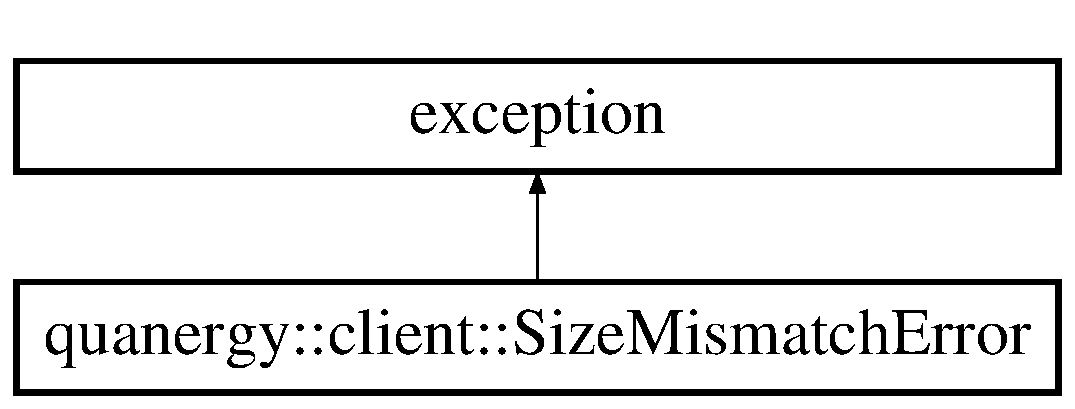
\includegraphics[height=2.000000cm]{structquanergy_1_1client_1_1SizeMismatchError}
\end{center}
\end{figure}
\subsection*{Public Member Functions}
\begin{DoxyCompactItemize}
\item 
\hypertarget{structquanergy_1_1client_1_1SizeMismatchError_a421f9bb14d8a01e1e656a19558ac200d}{virtual const char $\ast$ {\bfseries what} () const   throw ()}\label{structquanergy_1_1client_1_1SizeMismatchError_a421f9bb14d8a01e1e656a19558ac200d}

\end{DoxyCompactItemize}


\subsection{Detailed Description}
packet size doesn't match data description 

The documentation for this struct was generated from the following file\-:\begin{DoxyCompactItemize}
\item 
\hyperlink{exceptions_8h}{exceptions.\-h}\end{DoxyCompactItemize}

\hypertarget{structquanergy_1_1client_1_1SocketBindError}{\section{quanergy\-:\-:client\-:\-:Socket\-Bind\-Error Struct Reference}
\label{structquanergy_1_1client_1_1SocketBindError}\index{quanergy\-::client\-::\-Socket\-Bind\-Error@{quanergy\-::client\-::\-Socket\-Bind\-Error}}
}


error binding to socket  




{\ttfamily \#include $<$exceptions.\-h$>$}

Inheritance diagram for quanergy\-:\-:client\-:\-:Socket\-Bind\-Error\-:\begin{figure}[H]
\begin{center}
\leavevmode
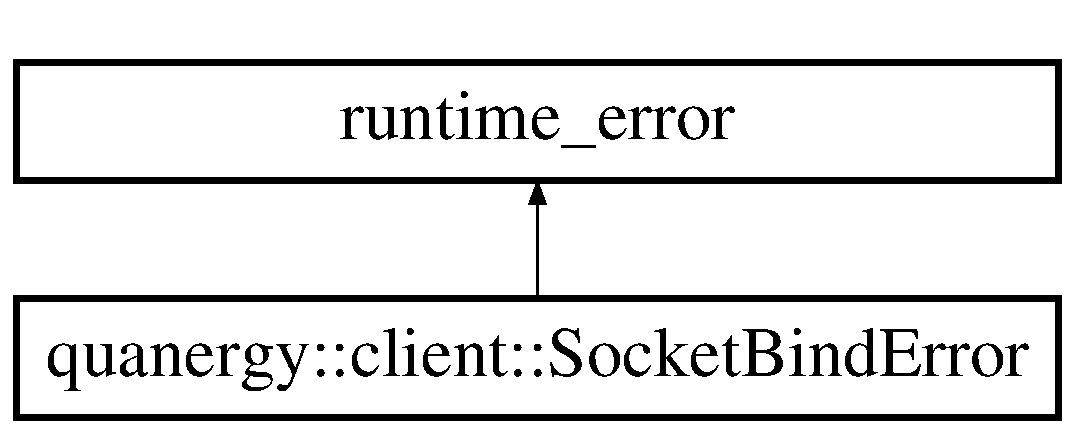
\includegraphics[height=2.000000cm]{structquanergy_1_1client_1_1SocketBindError}
\end{center}
\end{figure}
\subsection*{Public Member Functions}
\begin{DoxyCompactItemize}
\item 
\hypertarget{structquanergy_1_1client_1_1SocketBindError_a88d4f5b5c289d05b8fc83fde1a0a2a7d}{{\bfseries Socket\-Bind\-Error} (const std\-::string \&message)}\label{structquanergy_1_1client_1_1SocketBindError_a88d4f5b5c289d05b8fc83fde1a0a2a7d}

\end{DoxyCompactItemize}


\subsection{Detailed Description}
error binding to socket 

The documentation for this struct was generated from the following file\-:\begin{DoxyCompactItemize}
\item 
\hyperlink{exceptions_8h}{exceptions.\-h}\end{DoxyCompactItemize}

\hypertarget{structquanergy_1_1client_1_1SocketReadError}{\section{quanergy\-:\-:client\-:\-:Socket\-Read\-Error Struct Reference}
\label{structquanergy_1_1client_1_1SocketReadError}\index{quanergy\-::client\-::\-Socket\-Read\-Error@{quanergy\-::client\-::\-Socket\-Read\-Error}}
}


error reading from socket  




{\ttfamily \#include $<$exceptions.\-h$>$}

Inheritance diagram for quanergy\-:\-:client\-:\-:Socket\-Read\-Error\-:\begin{figure}[H]
\begin{center}
\leavevmode
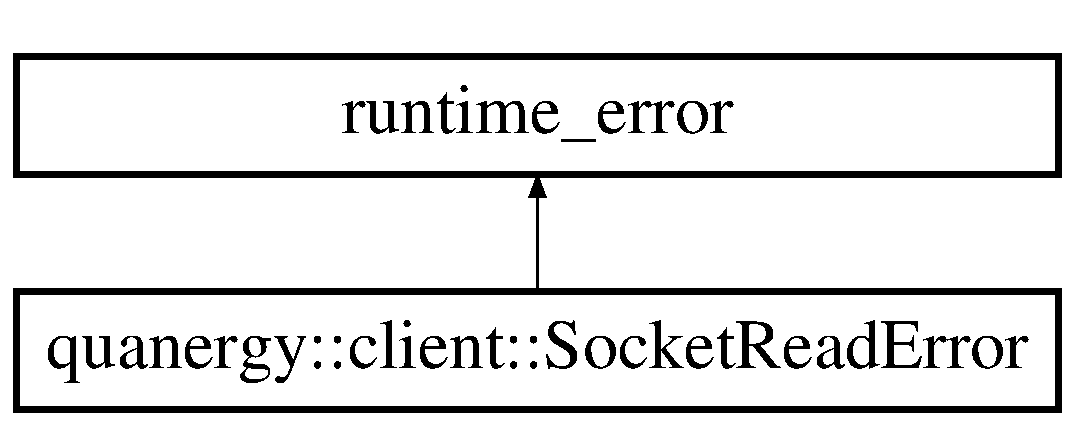
\includegraphics[height=2.000000cm]{structquanergy_1_1client_1_1SocketReadError}
\end{center}
\end{figure}
\subsection*{Public Member Functions}
\begin{DoxyCompactItemize}
\item 
\hypertarget{structquanergy_1_1client_1_1SocketReadError_a756263e78118dbdbce69d19377c179f8}{{\bfseries Socket\-Read\-Error} (const std\-::string \&message)}\label{structquanergy_1_1client_1_1SocketReadError_a756263e78118dbdbce69d19377c179f8}

\end{DoxyCompactItemize}


\subsection{Detailed Description}
error reading from socket 

The documentation for this struct was generated from the following file\-:\begin{DoxyCompactItemize}
\item 
\hyperlink{exceptions_8h}{exceptions.\-h}\end{DoxyCompactItemize}

\hypertarget{classquanergy_1_1client_1_1TCPClient}{\section{quanergy\-:\-:client\-:\-:T\-C\-P\-Client$<$ H\-E\-A\-D\-E\-R $>$ Class Template Reference}
\label{classquanergy_1_1client_1_1TCPClient}\index{quanergy\-::client\-::\-T\-C\-P\-Client$<$ H\-E\-A\-D\-E\-R $>$@{quanergy\-::client\-::\-T\-C\-P\-Client$<$ H\-E\-A\-D\-E\-R $>$}}
}


\hyperlink{classquanergy_1_1client_1_1TCPClient}{T\-C\-P\-Client} is a generic T\-C\-P data receiver that outputs packets based on header.  




{\ttfamily \#include $<$tcp\-\_\-client.\-h$>$}

\subsection*{Public Types}
\begin{DoxyCompactItemize}
\item 
\hypertarget{classquanergy_1_1client_1_1TCPClient_accb45d0241bc624ad63cf538b1585303}{typedef std\-::shared\-\_\-ptr\\*
$<$ std\-::vector$<$ char $>$ $>$ {\bfseries Result\-Type}}\label{classquanergy_1_1client_1_1TCPClient_accb45d0241bc624ad63cf538b1585303}

\item 
\hypertarget{classquanergy_1_1client_1_1TCPClient_a7b6902ce00b83a91c45162a7f718a64d}{typedef H\-E\-A\-D\-E\-R \hyperlink{classquanergy_1_1client_1_1TCPClient_a7b6902ce00b83a91c45162a7f718a64d}{Header\-Type}}\label{classquanergy_1_1client_1_1TCPClient_a7b6902ce00b83a91c45162a7f718a64d}

\begin{DoxyCompactList}\small\item\em give access to H\-E\-A\-D\-E\-R to derived classes \end{DoxyCompactList}\item 
\hypertarget{classquanergy_1_1client_1_1TCPClient_aa1754d14fea33b06a40a63b42b0e560c}{typedef \\*
boost\-::signals2\-::signal$<$ void(const \\*
Result\-Type \&)$>$ \hyperlink{classquanergy_1_1client_1_1TCPClient_aa1754d14fea33b06a40a63b42b0e560c}{Signal}}\label{classquanergy_1_1client_1_1TCPClient_aa1754d14fea33b06a40a63b42b0e560c}

\begin{DoxyCompactList}\small\item\em The packet is output on a signal. \end{DoxyCompactList}\end{DoxyCompactItemize}
\subsection*{Public Member Functions}
\begin{DoxyCompactItemize}
\item 
\hypertarget{classquanergy_1_1client_1_1TCPClient_a7caac3128ee9ac21709cdc1541018514}{\hyperlink{classquanergy_1_1client_1_1TCPClient_a7caac3128ee9ac21709cdc1541018514}{T\-C\-P\-Client} (std\-::string const \&host, std\-::string const \&port, std\-::size\-\_\-t max\-\_\-queue\-\_\-size=100)}\label{classquanergy_1_1client_1_1TCPClient_a7caac3128ee9ac21709cdc1541018514}

\begin{DoxyCompactList}\small\item\em Constructor taking a host, port, and queue size. \end{DoxyCompactList}\item 
\hypertarget{classquanergy_1_1client_1_1TCPClient_a47e8a916773370abf09263ab56a4bd85}{{\bfseries T\-C\-P\-Client} (const \hyperlink{classquanergy_1_1client_1_1TCPClient}{T\-C\-P\-Client} \&)=delete}\label{classquanergy_1_1client_1_1TCPClient_a47e8a916773370abf09263ab56a4bd85}

\item 
\hypertarget{classquanergy_1_1client_1_1TCPClient_a25fe677b76c4cfb2bc9b2b9eeb65c088}{\hyperlink{classquanergy_1_1client_1_1TCPClient}{T\-C\-P\-Client} \& {\bfseries operator=} (const \hyperlink{classquanergy_1_1client_1_1TCPClient}{T\-C\-P\-Client} \&)=delete}\label{classquanergy_1_1client_1_1TCPClient_a25fe677b76c4cfb2bc9b2b9eeb65c088}

\item 
\hypertarget{classquanergy_1_1client_1_1TCPClient_a80d8ce7142ef21da286976194becd6a9}{boost\-::signals2\-::connection \hyperlink{classquanergy_1_1client_1_1TCPClient_a80d8ce7142ef21da286976194becd6a9}{connect} (const typename Signal\-::slot\-\_\-type \&subscriber)}\label{classquanergy_1_1client_1_1TCPClient_a80d8ce7142ef21da286976194becd6a9}

\begin{DoxyCompactList}\small\item\em Connect a slot to the signal which will be emitted when a new R\-E\-S\-U\-L\-T is available. \end{DoxyCompactList}\item 
\hypertarget{classquanergy_1_1client_1_1TCPClient_ade508b6561dce937cffbb43390ff23c2}{virtual void \hyperlink{classquanergy_1_1client_1_1TCPClient_ade508b6561dce937cffbb43390ff23c2}{run} ()}\label{classquanergy_1_1client_1_1TCPClient_ade508b6561dce937cffbb43390ff23c2}

\begin{DoxyCompactList}\small\item\em Starts processing the Quanergy packets. \end{DoxyCompactList}\item 
\hypertarget{classquanergy_1_1client_1_1TCPClient_a96bbbcb279b343854262f521ac55ec86}{virtual void \hyperlink{classquanergy_1_1client_1_1TCPClient_a96bbbcb279b343854262f521ac55ec86}{stop} ()}\label{classquanergy_1_1client_1_1TCPClient_a96bbbcb279b343854262f521ac55ec86}

\begin{DoxyCompactList}\small\item\em Stops processing the Quanergy packets. \end{DoxyCompactList}\end{DoxyCompactItemize}
\subsection*{Protected Member Functions}
\begin{DoxyCompactItemize}
\item 
\hypertarget{classquanergy_1_1client_1_1TCPClient_a682a68ceae7d329b9553436c42e5ab0a}{virtual void \hyperlink{classquanergy_1_1client_1_1TCPClient_a682a68ceae7d329b9553436c42e5ab0a}{start\-Data\-Connect} ()}\label{classquanergy_1_1client_1_1TCPClient_a682a68ceae7d329b9553436c42e5ab0a}

\begin{DoxyCompactList}\small\item\em Asynchronously wait for connection. \end{DoxyCompactList}\item 
\hypertarget{classquanergy_1_1client_1_1TCPClient_a8f586dd803470de5c70a78d13c9ed66a}{virtual void \hyperlink{classquanergy_1_1client_1_1TCPClient_a8f586dd803470de5c70a78d13c9ed66a}{start\-Data\-Read} ()}\label{classquanergy_1_1client_1_1TCPClient_a8f586dd803470de5c70a78d13c9ed66a}

\begin{DoxyCompactList}\small\item\em Asynchronously read from socket. \end{DoxyCompactList}\item 
\hypertarget{classquanergy_1_1client_1_1TCPClient_a6fef2c07f3985c5bc646933d58542475}{virtual void \hyperlink{classquanergy_1_1client_1_1TCPClient_a6fef2c07f3985c5bc646933d58542475}{handle\-Read\-Header} (const boost\-::system\-::error\-\_\-code \&error)}\label{classquanergy_1_1client_1_1TCPClient_a6fef2c07f3985c5bc646933d58542475}

\begin{DoxyCompactList}\small\item\em Handle read of packet header. \end{DoxyCompactList}\item 
\hypertarget{classquanergy_1_1client_1_1TCPClient_abe037d34a60b07c3af30cabecede4fdc}{virtual void \hyperlink{classquanergy_1_1client_1_1TCPClient_abe037d34a60b07c3af30cabecede4fdc}{handle\-Read\-Body} (const boost\-::system\-::error\-\_\-code \&error)}\label{classquanergy_1_1client_1_1TCPClient_abe037d34a60b07c3af30cabecede4fdc}

\begin{DoxyCompactList}\small\item\em Handle read of packet body. \end{DoxyCompactList}\item 
\hypertarget{classquanergy_1_1client_1_1TCPClient_a2ad2a7e7f4d541a3b0b23cf6489e5ff1}{virtual void \hyperlink{classquanergy_1_1client_1_1TCPClient_a2ad2a7e7f4d541a3b0b23cf6489e5ff1}{signal\-Packets} ()}\label{classquanergy_1_1client_1_1TCPClient_a2ad2a7e7f4d541a3b0b23cf6489e5ff1}

\begin{DoxyCompactList}\small\item\em Pulls packets off buffer queue and calls signal. \end{DoxyCompactList}\end{DoxyCompactItemize}
\subsection*{Protected Attributes}
\begin{DoxyCompactItemize}
\item 
\hypertarget{classquanergy_1_1client_1_1TCPClient_a3169f1eb8c9ed9b452cd12ba4d51cd44}{std\-::unique\-\_\-ptr\\*
$<$ boost\-::asio\-::ip\-::tcp\-::socket $>$ {\bfseries read\-\_\-socket\-\_\-}}\label{classquanergy_1_1client_1_1TCPClient_a3169f1eb8c9ed9b452cd12ba4d51cd44}

\item 
\hypertarget{classquanergy_1_1client_1_1TCPClient_ab99a028a1b6efe74a8f62ed1f9323449}{std\-::vector$<$ char $>$ {\bfseries buff\-\_\-}}\label{classquanergy_1_1client_1_1TCPClient_ab99a028a1b6efe74a8f62ed1f9323449}

\end{DoxyCompactItemize}


\subsection{Detailed Description}
\subsubsection*{template$<$class H\-E\-A\-D\-E\-R$>$class quanergy\-::client\-::\-T\-C\-P\-Client$<$ H\-E\-A\-D\-E\-R $>$}

\hyperlink{classquanergy_1_1client_1_1TCPClient}{T\-C\-P\-Client} is a generic T\-C\-P data receiver that outputs packets based on header. 


\begin{DoxyTemplParams}{Template Parameters}
{\em H\-E\-A\-D\-E\-R} & is the packet header type \\
\hline
\end{DoxyTemplParams}
\begin{DoxyAttention}{Attention}
The following two functions must be provided for H\-E\-A\-D\-E\-R type bool validate\-Header(const H\-E\-A\-D\-E\-R\&); // returns true if valid std\-::size\-\_\-t get\-Packet\-Size(const H\-E\-A\-D\-E\-R\&); // returns the size of the full packet including header 
\end{DoxyAttention}


The documentation for this class was generated from the following files\-:\begin{DoxyCompactItemize}
\item 
\hyperlink{tcp__client_8h}{tcp\-\_\-client.\-h}\item 
tcp\-\_\-client.\-hpp\end{DoxyCompactItemize}

\hypertarget{structquanergy_1_1client_1_1VariadicPacketParser}{\section{quanergy\-:\-:client\-:\-:Variadic\-Packet\-Parser$<$ R\-E\-S\-U\-L\-T, P\-A\-R\-S\-E\-R\-S $>$ Struct Template Reference}
\label{structquanergy_1_1client_1_1VariadicPacketParser}\index{quanergy\-::client\-::\-Variadic\-Packet\-Parser$<$ R\-E\-S\-U\-L\-T, P\-A\-R\-S\-E\-R\-S $>$@{quanergy\-::client\-::\-Variadic\-Packet\-Parser$<$ R\-E\-S\-U\-L\-T, P\-A\-R\-S\-E\-R\-S $>$}}
}
Inheritance diagram for quanergy\-:\-:client\-:\-:Variadic\-Packet\-Parser$<$ R\-E\-S\-U\-L\-T, P\-A\-R\-S\-E\-R\-S $>$\-:\begin{figure}[H]
\begin{center}
\leavevmode
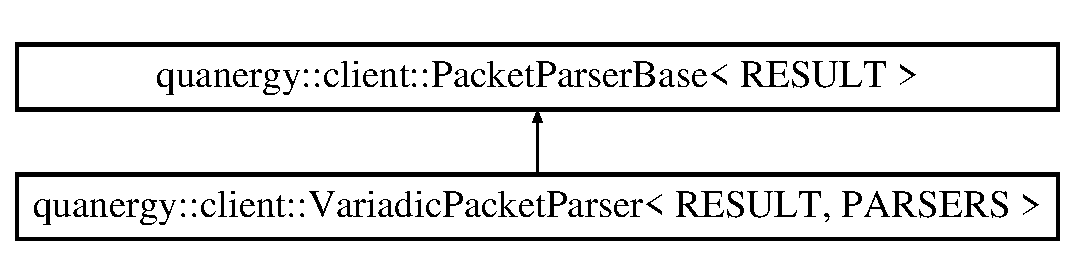
\includegraphics[height=2.000000cm]{structquanergy_1_1client_1_1VariadicPacketParser}
\end{center}
\end{figure}
\subsection*{Public Types}
\begin{DoxyCompactItemize}
\item 
\hypertarget{structquanergy_1_1client_1_1VariadicPacketParser_aad48760d6d29342cf8358371b2fea630}{typedef R\-E\-S\-U\-L\-T {\bfseries Result\-Type}}\label{structquanergy_1_1client_1_1VariadicPacketParser_aad48760d6d29342cf8358371b2fea630}

\end{DoxyCompactItemize}
\subsection*{Public Member Functions}
\begin{DoxyCompactItemize}
\item 
\hypertarget{structquanergy_1_1client_1_1VariadicPacketParser_a76139502de94d8f94bc9d5b9ac749695}{{\footnotesize template$<$std\-::size\-\_\-t I$>$ }\\auto \hyperlink{structquanergy_1_1client_1_1VariadicPacketParser_a76139502de94d8f94bc9d5b9ac749695}{get} () -\/$>$ decltype(std\-::get$<$ I $>$(std\-::tuple$<$ P\-A\-R\-S\-E\-R\-S...$>$()))\&}\label{structquanergy_1_1client_1_1VariadicPacketParser_a76139502de94d8f94bc9d5b9ac749695}

\begin{DoxyCompactList}\small\item\em provide access to the individual parsers \end{DoxyCompactList}\item 
\hypertarget{structquanergy_1_1client_1_1VariadicPacketParser_a58a6ec899ab3ee7f2fbd92b4d45082eb}{virtual bool \hyperlink{structquanergy_1_1client_1_1VariadicPacketParser_a58a6ec899ab3ee7f2fbd92b4d45082eb}{validate\-Parse} (const std\-::vector$<$ char $>$ \&packet, R\-E\-S\-U\-L\-T \&result)}\label{structquanergy_1_1client_1_1VariadicPacketParser_a58a6ec899ab3ee7f2fbd92b4d45082eb}

\begin{DoxyCompactList}\small\item\em iterate through parsers to find first match and parse \end{DoxyCompactList}\item 
\hypertarget{structquanergy_1_1client_1_1VariadicPacketParser_a5b53284ba762fc0d9355d28f552bd674}{virtual bool \hyperlink{structquanergy_1_1client_1_1VariadicPacketParser_a5b53284ba762fc0d9355d28f552bd674}{validate} (const std\-::vector$<$ char $>$ \&packet)}\label{structquanergy_1_1client_1_1VariadicPacketParser_a5b53284ba762fc0d9355d28f552bd674}

\begin{DoxyCompactList}\small\item\em iterate through parsers to see if there is a match \end{DoxyCompactList}\item 
\hypertarget{structquanergy_1_1client_1_1VariadicPacketParser_af66c0c1212314c43f6a183e7a4711e44}{virtual bool \hyperlink{structquanergy_1_1client_1_1VariadicPacketParser_af66c0c1212314c43f6a183e7a4711e44}{parse} (const std\-::vector$<$ char $>$ \&packet, R\-E\-S\-U\-L\-T \&result)}\label{structquanergy_1_1client_1_1VariadicPacketParser_af66c0c1212314c43f6a183e7a4711e44}

\begin{DoxyCompactList}\small\item\em parse using validate\-Parse but catch throw \end{DoxyCompactList}\end{DoxyCompactItemize}


The documentation for this struct was generated from the following file\-:\begin{DoxyCompactItemize}
\item 
\hyperlink{variadic__packet__parser_8h}{variadic\-\_\-packet\-\_\-parser.\-h}\end{DoxyCompactItemize}

\hypertarget{classVisualizerModule}{\section{Visualizer\-Module Class Reference}
\label{classVisualizerModule}\index{Visualizer\-Module@{Visualizer\-Module}}
}


struct contains the intelligence of the test application  




{\ttfamily \#include $<$visualizer\-\_\-module.\-h$>$}

\subsection*{Public Member Functions}
\begin{DoxyCompactItemize}
\item 
\hyperlink{classVisualizerModule_a133805b5b07aaedc10eb9315cb6d3f5f}{Visualizer\-Module} ()
\item 
\hypertarget{classVisualizerModule_aa61d4ab50f76c2c1f9cceb6389db2db2}{void {\bfseries slot} (const quanergy\-::\-Point\-Cloud\-X\-Y\-Z\-I\-R\-Const\-Ptr \&new\-\_\-cloud)}\label{classVisualizerModule_aa61d4ab50f76c2c1f9cceb6389db2db2}

\item 
void \hyperlink{classVisualizerModule_a386e56c93e95ce3381dd99691ce53a0b}{run} ()
\begin{DoxyCompactList}\small\item\em run the application \end{DoxyCompactList}\item 
\hypertarget{classVisualizerModule_acd1bbd20ca2637ffd30e5e5693831193}{void \hyperlink{classVisualizerModule_acd1bbd20ca2637ffd30e5e5693831193}{stop} ()}\label{classVisualizerModule_acd1bbd20ca2637ffd30e5e5693831193}

\begin{DoxyCompactList}\small\item\em stop the application \end{DoxyCompactList}\end{DoxyCompactItemize}


\subsection{Detailed Description}
struct contains the intelligence of the test application 

\subsection{Constructor \& Destructor Documentation}
\hypertarget{classVisualizerModule_a133805b5b07aaedc10eb9315cb6d3f5f}{\index{Visualizer\-Module@{Visualizer\-Module}!Visualizer\-Module@{Visualizer\-Module}}
\index{Visualizer\-Module@{Visualizer\-Module}!VisualizerModule@{Visualizer\-Module}}
\subsubsection[{Visualizer\-Module}]{\setlength{\rightskip}{0pt plus 5cm}Visualizer\-Module\-::\-Visualizer\-Module (
\begin{DoxyParamCaption}
{}
\end{DoxyParamCaption}
)}}\label{classVisualizerModule_a133805b5b07aaedc10eb9315cb6d3f5f}
basic visualization setup 

\subsection{Member Function Documentation}
\hypertarget{classVisualizerModule_a386e56c93e95ce3381dd99691ce53a0b}{\index{Visualizer\-Module@{Visualizer\-Module}!run@{run}}
\index{run@{run}!VisualizerModule@{Visualizer\-Module}}
\subsubsection[{run}]{\setlength{\rightskip}{0pt plus 5cm}void Visualizer\-Module\-::run (
\begin{DoxyParamCaption}
{}
\end{DoxyParamCaption}
)}}\label{classVisualizerModule_a386e56c93e95ce3381dd99691ce53a0b}


run the application 

spin loop for updating visualizer 

The documentation for this class was generated from the following files\-:\begin{DoxyCompactItemize}
\item 
visualizer\-\_\-module.\-h\item 
visualizer\-\_\-module.\-cpp\end{DoxyCompactItemize}

\chapter{File Documentation}
\hypertarget{data__packet__00_8h}{\section{data\-\_\-packet\-\_\-00.\-h File Reference}
\label{data__packet__00_8h}\index{data\-\_\-packet\-\_\-00.\-h@{data\-\_\-packet\-\_\-00.\-h}}
}


Provide deserialization functionality for data packet type 0x00.  


{\ttfamily \#include $<$quanergy/client/packet\-\_\-header.\-h$>$}\\*
{\ttfamily \#include $<$quanergy/client/m8\-\_\-data\-\_\-packet.\-h$>$}\\*
\subsection*{Classes}
\begin{DoxyCompactItemize}
\item 
struct \hyperlink{structquanergy_1_1client_1_1DataPacket00}{quanergy\-::client\-::\-Data\-Packet00}
\begin{DoxyCompactList}\small\item\em data packet 0x00 \end{DoxyCompactList}\end{DoxyCompactItemize}
\subsection*{Namespaces}
\begin{DoxyCompactItemize}
\item 
\hyperlink{namespacequanergy}{quanergy}
\begin{DoxyCompactList}\small\item\em Variadic\-Packet\-Parer takes a list of parsers and iterates through them. \end{DoxyCompactList}\end{DoxyCompactItemize}
\subsection*{Functions}
\begin{DoxyCompactItemize}
\item 
\hypertarget{namespacequanergy_1_1client_a48e49604e5c7bf2353ebfc944ad8df09}{D\-L\-L\-E\-X\-P\-O\-R\-T void {\bfseries quanergy\-::client\-::deserialize} (const char $\ast$network\-\_\-buffer, M8\-Firing\-Data \&object)}\label{namespacequanergy_1_1client_a48e49604e5c7bf2353ebfc944ad8df09}

\item 
\hypertarget{namespacequanergy_1_1client_adb99314ce6a8d192c217a123d3980c02}{D\-L\-L\-E\-X\-P\-O\-R\-T void {\bfseries quanergy\-::client\-::deserialize} (const char $\ast$network\-\_\-buffer, M8\-Data\-Packet \&object)}\label{namespacequanergy_1_1client_adb99314ce6a8d192c217a123d3980c02}

\item 
\hypertarget{namespacequanergy_1_1client_ac1d6806171496fac59dd734b6e498bf7}{D\-L\-L\-E\-X\-P\-O\-R\-T void {\bfseries quanergy\-::client\-::deserialize} (const char $\ast$network\-\_\-buffer, Data\-Packet00 \&object)}\label{namespacequanergy_1_1client_ac1d6806171496fac59dd734b6e498bf7}

\end{DoxyCompactItemize}


\subsection{Detailed Description}
Provide deserialization functionality for data packet type 0x00. data packet 00 is a wrapper for the old m8 data with the new header. 
\hypertarget{data__packet__01_8h}{\section{data\-\_\-packet\-\_\-01.\-h File Reference}
\label{data__packet__01_8h}\index{data\-\_\-packet\-\_\-01.\-h@{data\-\_\-packet\-\_\-01.\-h}}
}


Provide deserialization functionality for data packet type 0x01.  


{\ttfamily \#include $<$iostream$>$}\\*
{\ttfamily \#include $<$quanergy/client/packet\-\_\-header.\-h$>$}\\*
\subsection*{Classes}
\begin{DoxyCompactItemize}
\item 
struct \hyperlink{structquanergy_1_1client_1_1DataHeader01}{quanergy\-::client\-::\-Data\-Header01}
\begin{DoxyCompactList}\small\item\em data header 0x01 \end{DoxyCompactList}\item 
struct \hyperlink{structquanergy_1_1client_1_1DataPoint01}{quanergy\-::client\-::\-Data\-Point01}
\begin{DoxyCompactList}\small\item\em data point 0x01 \end{DoxyCompactList}\item 
struct \hyperlink{structquanergy_1_1client_1_1DataPacket01}{quanergy\-::client\-::\-Data\-Packet01}
\begin{DoxyCompactList}\small\item\em data packet 0x01 \end{DoxyCompactList}\end{DoxyCompactItemize}
\subsection*{Namespaces}
\begin{DoxyCompactItemize}
\item 
\hyperlink{namespacequanergy}{quanergy}
\begin{DoxyCompactList}\small\item\em Variadic\-Packet\-Parer takes a list of parsers and iterates through them. \end{DoxyCompactList}\end{DoxyCompactItemize}
\subsection*{Functions}
\begin{DoxyCompactItemize}
\item 
\hypertarget{namespacequanergy_1_1client_ad41db393ba8b4a3e27abdeb7a94a49ec}{D\-L\-L\-E\-X\-P\-O\-R\-T void {\bfseries quanergy\-::client\-::deserialize} (const char $\ast$network\-\_\-buffer, Data\-Header01 \&object)}\label{namespacequanergy_1_1client_ad41db393ba8b4a3e27abdeb7a94a49ec}

\item 
\hypertarget{namespacequanergy_1_1client_a537a622b9d7331706a5ed745c64bc5dd}{D\-L\-L\-E\-X\-P\-O\-R\-T void {\bfseries quanergy\-::client\-::deserialize} (const char $\ast$network\-\_\-buffer, Data\-Point01 \&object)}\label{namespacequanergy_1_1client_a537a622b9d7331706a5ed745c64bc5dd}

\item 
\hypertarget{namespacequanergy_1_1client_a5e3f721f524c89c835b2152c895e1b71}{D\-L\-L\-E\-X\-P\-O\-R\-T void {\bfseries quanergy\-::client\-::deserialize} (const char $\ast$network\-\_\-buffer, Data\-Packet01 \&object)}\label{namespacequanergy_1_1client_a5e3f721f524c89c835b2152c895e1b71}

\end{DoxyCompactItemize}


\subsection{Detailed Description}
Provide deserialization functionality for data packet type 0x01. 
\hypertarget{data__packet__04_8h}{\section{data\-\_\-packet\-\_\-04.\-h File Reference}
\label{data__packet__04_8h}\index{data\-\_\-packet\-\_\-04.\-h@{data\-\_\-packet\-\_\-04.\-h}}
}


Data structure for Reduced-\/\-Bandwidth M8 Packet (04)  


{\ttfamily \#include $<$quanergy/client/packet\-\_\-header.\-h$>$}\\*
{\ttfamily \#include $<$quanergy/client/m8\-\_\-data\-\_\-packet.\-h$>$}\\*
\subsection*{Classes}
\begin{DoxyCompactItemize}
\item 
struct \hyperlink{structquanergy_1_1client_1_1M8DataPacket04Header}{quanergy\-::client\-::\-M8\-Data\-Packet04\-Header}
\item 
struct \hyperlink{structquanergy_1_1client_1_1M8FiringData04}{quanergy\-::client\-::\-M8\-Firing\-Data04}
\item 
struct \hyperlink{structquanergy_1_1client_1_1M8DataPacket04}{quanergy\-::client\-::\-M8\-Data\-Packet04}
\item 
struct \hyperlink{structquanergy_1_1client_1_1DataPacket04}{quanergy\-::client\-::\-Data\-Packet04}
\end{DoxyCompactItemize}
\subsection*{Namespaces}
\begin{DoxyCompactItemize}
\item 
\hyperlink{namespacequanergy}{quanergy}
\begin{DoxyCompactList}\small\item\em Variadic\-Packet\-Parer takes a list of parsers and iterates through them. \end{DoxyCompactList}\end{DoxyCompactItemize}
\subsection*{Functions}
\begin{DoxyCompactItemize}
\item 
\hypertarget{namespacequanergy_1_1client_aad962d4ea0f96db3cca1d679e2c3f478}{D\-L\-L\-E\-X\-P\-O\-R\-T void {\bfseries quanergy\-::client\-::deserialize} (const char $\ast$network\-\_\-buffer, M8\-Data\-Packet04 \&object)}\label{namespacequanergy_1_1client_aad962d4ea0f96db3cca1d679e2c3f478}

\item 
\hypertarget{namespacequanergy_1_1client_a7a6d111a54d0822e916d069e48a0b60a}{D\-L\-L\-E\-X\-P\-O\-R\-T void {\bfseries quanergy\-::client\-::deserialize} (const char $\ast$network\-\_\-buffer, Data\-Packet04 \&object)}\label{namespacequanergy_1_1client_a7a6d111a54d0822e916d069e48a0b60a}

\end{DoxyCompactItemize}


\subsection{Detailed Description}
Data structure for Reduced-\/\-Bandwidth M8 Packet (04) 
\hypertarget{data__packet__parser_8h}{\section{data\-\_\-packet\-\_\-parser.\-h File Reference}
\label{data__packet__parser_8h}\index{data\-\_\-packet\-\_\-parser.\-h@{data\-\_\-packet\-\_\-parser.\-h}}
}


specialize packet parser for H\-V\-D\-I\-R data out  


{\ttfamily \#include $<$quanergy/parsers/packet\-\_\-parser.\-h$>$}\\*
{\ttfamily \#include $<$quanergy/common/pointcloud\-\_\-types.\-h$>$}\\*
\subsection*{Classes}
\begin{DoxyCompactItemize}
\item 
struct \hyperlink{structquanergy_1_1client_1_1DataPacketParser}{quanergy\-::client\-::\-Data\-Packet\-Parser}
\begin{DoxyCompactList}\small\item\em base class for data packet parsers \end{DoxyCompactList}\end{DoxyCompactItemize}
\subsection*{Namespaces}
\begin{DoxyCompactItemize}
\item 
\hyperlink{namespacequanergy}{quanergy}
\begin{DoxyCompactList}\small\item\em Variadic\-Packet\-Parer takes a list of parsers and iterates through them. \end{DoxyCompactList}\end{DoxyCompactItemize}


\subsection{Detailed Description}
specialize packet parser for H\-V\-D\-I\-R data out 
\hypertarget{data__packet__parser__00_8h}{\section{data\-\_\-packet\-\_\-parser\-\_\-00.\-h File Reference}
\label{data__packet__parser__00_8h}\index{data\-\_\-packet\-\_\-parser\-\_\-00.\-h@{data\-\_\-packet\-\_\-parser\-\_\-00.\-h}}
}


Provide pointcloud parser functionality for data type 0x00.  


{\ttfamily \#include $<$quanergy/parsers/packet\-\_\-parser.\-h$>$}\\*
{\ttfamily \#include $<$quanergy/common/pointcloud\-\_\-types.\-h$>$}\\*
{\ttfamily \#include $<$quanergy/parsers/data\-\_\-packet\-\_\-00.\-h$>$}\\*
{\ttfamily \#include $<$quanergy/parsers/data\-\_\-packet\-\_\-parser\-\_\-m8.\-h$>$}\\*
\subsection*{Classes}
\begin{DoxyCompactItemize}
\item 
struct \hyperlink{structquanergy_1_1client_1_1DataPacketParser00}{quanergy\-::client\-::\-Data\-Packet\-Parser00}
\end{DoxyCompactItemize}
\subsection*{Namespaces}
\begin{DoxyCompactItemize}
\item 
\hyperlink{namespacequanergy}{quanergy}
\begin{DoxyCompactList}\small\item\em Variadic\-Packet\-Parer takes a list of parsers and iterates through them. \end{DoxyCompactList}\end{DoxyCompactItemize}


\subsection{Detailed Description}
Provide pointcloud parser functionality for data type 0x00. 
\hypertarget{data__packet__parser__01_8h}{\section{data\-\_\-packet\-\_\-parser\-\_\-01.\-h File Reference}
\label{data__packet__parser__01_8h}\index{data\-\_\-packet\-\_\-parser\-\_\-01.\-h@{data\-\_\-packet\-\_\-parser\-\_\-01.\-h}}
}


Provide pointcloud parser functionality for data type 0x01.  


{\ttfamily \#include $<$limits$>$}\\*
{\ttfamily \#include $<$quanergy/parsers/data\-\_\-packet\-\_\-parser.\-h$>$}\\*
{\ttfamily \#include $<$quanergy/parsers/data\-\_\-packet\-\_\-01.\-h$>$}\\*
\subsection*{Classes}
\begin{DoxyCompactItemize}
\item 
struct \hyperlink{structquanergy_1_1client_1_1DataPacketParser01}{quanergy\-::client\-::\-Data\-Packet\-Parser01}
\end{DoxyCompactItemize}
\subsection*{Namespaces}
\begin{DoxyCompactItemize}
\item 
\hyperlink{namespacequanergy}{quanergy}
\begin{DoxyCompactList}\small\item\em Variadic\-Packet\-Parer takes a list of parsers and iterates through them. \end{DoxyCompactList}\end{DoxyCompactItemize}


\subsection{Detailed Description}
Provide pointcloud parser functionality for data type 0x01. 
\hypertarget{data__packet__parser__04_8h}{\section{data\-\_\-packet\-\_\-parser\-\_\-04.\-h File Reference}
\label{data__packet__parser__04_8h}\index{data\-\_\-packet\-\_\-parser\-\_\-04.\-h@{data\-\_\-packet\-\_\-parser\-\_\-04.\-h}}
}


Provide pointcloud parser functionality for data type 0x04.  


{\ttfamily \#include $<$quanergy/parsers/packet\-\_\-parser.\-h$>$}\\*
{\ttfamily \#include $<$quanergy/parsers/data\-\_\-packet\-\_\-04.\-h$>$}\\*
{\ttfamily \#include $<$quanergy/parsers/data\-\_\-packet\-\_\-parser\-\_\-m8.\-h$>$}\\*
\subsection*{Classes}
\begin{DoxyCompactItemize}
\item 
struct \hyperlink{structquanergy_1_1client_1_1DataPacketParser04}{quanergy\-::client\-::\-Data\-Packet\-Parser04}
\end{DoxyCompactItemize}
\subsection*{Namespaces}
\begin{DoxyCompactItemize}
\item 
\hyperlink{namespacequanergy}{quanergy}
\begin{DoxyCompactList}\small\item\em Variadic\-Packet\-Parer takes a list of parsers and iterates through them. \end{DoxyCompactList}\end{DoxyCompactItemize}


\subsection{Detailed Description}
Provide pointcloud parser functionality for data type 0x04. 
\hypertarget{data__packet__parser__m8_8h}{\section{data\-\_\-packet\-\_\-parser\-\_\-m8.\-h File Reference}
\label{data__packet__parser__m8_8h}\index{data\-\_\-packet\-\_\-parser\-\_\-m8.\-h@{data\-\_\-packet\-\_\-parser\-\_\-m8.\-h}}
}


Provide pointcloud parser functionality for m8 data.  


{\ttfamily \#include $<$quanergy/parsers/data\-\_\-packet\-\_\-parser.\-h$>$}\\*
{\ttfamily \#include $<$quanergy/client/m8\-\_\-data\-\_\-packet.\-h$>$}\\*
\subsection*{Classes}
\begin{DoxyCompactItemize}
\item 
struct \hyperlink{structquanergy_1_1client_1_1DataPacketParserM8}{quanergy\-::client\-::\-Data\-Packet\-Parser\-M8}
\begin{DoxyCompactList}\small\item\em Not a specialization because it is intended to be used by others. \end{DoxyCompactList}\end{DoxyCompactItemize}
\subsection*{Namespaces}
\begin{DoxyCompactItemize}
\item 
\hyperlink{namespacequanergy}{quanergy}
\begin{DoxyCompactList}\small\item\em Variadic\-Packet\-Parer takes a list of parsers and iterates through them. \end{DoxyCompactList}\end{DoxyCompactItemize}
\subsection*{Variables}
\begin{DoxyCompactItemize}
\item 
const double {\bfseries quanergy\-::client\-::\-M8\-\_\-\-V\-E\-R\-T\-I\-C\-A\-L\-\_\-\-A\-N\-G\-L\-E\-S} \mbox{[}$\,$\mbox{]}
\item 
\hypertarget{namespacequanergy_1_1client_a9294cb396ffe8152f1dd449ca3a78376}{const std\-::int32\-\_\-t {\bfseries quanergy\-::client\-::\-M8\-\_\-\-N\-U\-M\-\_\-\-R\-O\-T\-\_\-\-A\-N\-G\-L\-E\-S} = 10400}\label{namespacequanergy_1_1client_a9294cb396ffe8152f1dd449ca3a78376}

\item 
\hypertarget{namespacequanergy_1_1client_a67e8967c821f51267a612ed0c55b8d4f}{const int {\bfseries quanergy\-::client\-::\-A\-L\-L\-\_\-\-R\-E\-T\-U\-R\-N\-S} = -\/1}\label{namespacequanergy_1_1client_a67e8967c821f51267a612ed0c55b8d4f}

\begin{DoxyCompactList}\small\item\em Used to specify 'all' returns. \end{DoxyCompactList}\end{DoxyCompactItemize}


\subsection{Detailed Description}
Provide pointcloud parser functionality for m8 data. 
\hypertarget{distance__filter_8h}{\section{distance\-\_\-filter.\-h File Reference}
\label{distance__filter_8h}\index{distance\-\_\-filter.\-h@{distance\-\_\-filter.\-h}}
}


Filters H\-V\-D\-I\-R points based on radius distance (by setting them to N\-A\-N).  


{\ttfamily \#include $<$memory$>$}\\*
{\ttfamily \#include $<$boost/signals2.\-hpp$>$}\\*
{\ttfamily \#include $<$pcl/point\-\_\-cloud.\-h$>$}\\*
{\ttfamily \#include $<$quanergy/common/point\-\_\-hvdir.\-h$>$}\\*
{\ttfamily \#include $<$quanergy/common/pointcloud\-\_\-types.\-h$>$}\\*
\subsection*{Classes}
\begin{DoxyCompactItemize}
\item 
struct \hyperlink{structquanergy_1_1client_1_1DistanceFilter}{quanergy\-::client\-::\-Distance\-Filter}
\end{DoxyCompactItemize}
\subsection*{Namespaces}
\begin{DoxyCompactItemize}
\item 
\hyperlink{namespacequanergy}{quanergy}
\begin{DoxyCompactList}\small\item\em Variadic\-Packet\-Parer takes a list of parsers and iterates through them. \end{DoxyCompactList}\end{DoxyCompactItemize}
\subsection*{Macros}
\begin{DoxyCompactItemize}
\item 
\hypertarget{distance__filter_8h_a808e08638be3cba36e36759e5b150de0}{\#define {\bfseries D\-L\-L\-E\-X\-P\-O\-R\-T}}\label{distance__filter_8h_a808e08638be3cba36e36759e5b150de0}

\item 
\hypertarget{distance__filter_8h_a17f2e729a629eee9f5b7371c357f5e25}{\#define {\bfseries T\-Y\-P\-E\-N\-A\-M\-E}~typename}\label{distance__filter_8h_a17f2e729a629eee9f5b7371c357f5e25}

\end{DoxyCompactItemize}


\subsection{Detailed Description}
Filters H\-V\-D\-I\-R points based on radius distance (by setting them to N\-A\-N). 
\hypertarget{exceptions_8h}{\section{exceptions.\-h File Reference}
\label{exceptions_8h}\index{exceptions.\-h@{exceptions.\-h}}
}


Define specific sensor client run-\/time exceptions.  


{\ttfamily \#include $<$stdexcept$>$}\\*
\subsection*{Classes}
\begin{DoxyCompactItemize}
\item 
struct \hyperlink{structquanergy_1_1client_1_1SocketBindError}{quanergy\-::client\-::\-Socket\-Bind\-Error}
\begin{DoxyCompactList}\small\item\em error binding to socket \end{DoxyCompactList}\item 
struct \hyperlink{structquanergy_1_1client_1_1SocketReadError}{quanergy\-::client\-::\-Socket\-Read\-Error}
\begin{DoxyCompactList}\small\item\em error reading from socket \end{DoxyCompactList}\item 
struct \hyperlink{structquanergy_1_1client_1_1InvalidHeaderError}{quanergy\-::client\-::\-Invalid\-Header\-Error}
\begin{DoxyCompactList}\small\item\em error parsing header \end{DoxyCompactList}\item 
struct \hyperlink{structquanergy_1_1client_1_1SizeMismatchError}{quanergy\-::client\-::\-Size\-Mismatch\-Error}
\begin{DoxyCompactList}\small\item\em packet size doesn't match data description \end{DoxyCompactList}\item 
struct \hyperlink{structquanergy_1_1client_1_1InvalidPacketError}{quanergy\-::client\-::\-Invalid\-Packet\-Error}
\begin{DoxyCompactList}\small\item\em Invalid packet. \end{DoxyCompactList}\item 
struct \hyperlink{structquanergy_1_1client_1_1InvalidDataTypeError}{quanergy\-::client\-::\-Invalid\-Data\-Type\-Error}
\begin{DoxyCompactList}\small\item\em Invalid data type in header; no parser available. \end{DoxyCompactList}\item 
struct \hyperlink{structquanergy_1_1client_1_1InvalidDataVersionError}{quanergy\-::client\-::\-Invalid\-Data\-Version\-Error}
\begin{DoxyCompactList}\small\item\em Invalid version for type. \end{DoxyCompactList}\item 
struct \hyperlink{structquanergy_1_1client_1_1FirmwareVersionMismatchError}{quanergy\-::client\-::\-Firmware\-Version\-Mismatch\-Error}
\begin{DoxyCompactList}\small\item\em Firmware versions on sensor don't match. \end{DoxyCompactList}\item 
struct \hyperlink{structquanergy_1_1client_1_1FirmwareWatchdogViolationError}{quanergy\-::client\-::\-Firmware\-Watchdog\-Violation\-Error}
\begin{DoxyCompactList}\small\item\em Firmware watchdog is not receiving an internal signal. \end{DoxyCompactList}\item 
struct \hyperlink{structquanergy_1_1client_1_1FirmwareUnknownError}{quanergy\-::client\-::\-Firmware\-Unknown\-Error}
\begin{DoxyCompactList}\small\item\em Firmware unknown error Raised for status bits that are not presently assigned. \end{DoxyCompactList}\item 
struct \hyperlink{structquanergy_1_1client_1_1InvalidDegreesPerCloud}{quanergy\-::client\-::\-Invalid\-Degrees\-Per\-Cloud}
\begin{DoxyCompactList}\small\item\em Degress per cloud must be 360 or less. \end{DoxyCompactList}\item 
struct \hyperlink{structquanergy_1_1client_1_1InvalidReturnSelection}{quanergy\-::client\-::\-Invalid\-Return\-Selection}
\begin{DoxyCompactList}\small\item\em Return selction must be less than M8\-\_\-\-N\-U\-M\-\_\-\-R\-E\-T\-U\-R\-N\-S. \end{DoxyCompactList}\item 
struct \hyperlink{structquanergy_1_1client_1_1ReturnIDMismatchError}{quanergy\-::client\-::\-Return\-I\-D\-Mismatch\-Error}
\begin{DoxyCompactList}\small\item\em Return I\-D coming from sensor doesn't match requested Return I\-D. \end{DoxyCompactList}\end{DoxyCompactItemize}
\subsection*{Namespaces}
\begin{DoxyCompactItemize}
\item 
\hyperlink{namespacequanergy}{quanergy}
\begin{DoxyCompactList}\small\item\em Variadic\-Packet\-Parer takes a list of parsers and iterates through them. \end{DoxyCompactList}\end{DoxyCompactItemize}


\subsection{Detailed Description}
Define specific sensor client run-\/time exceptions. 
\hypertarget{m8__data__packet_8h}{\section{m8\-\_\-data\-\_\-packet.\-h File Reference}
\label{m8__data__packet_8h}\index{m8\-\_\-data\-\_\-packet.\-h@{m8\-\_\-data\-\_\-packet.\-h}}
}


Provide definition of old m8 data packet.  


{\ttfamily \#include $<$cstdint$>$}\\*
\subsection*{Classes}
\begin{DoxyCompactItemize}
\item 
struct \hyperlink{structquanergy_1_1client_1_1M8FiringData}{quanergy\-::client\-::\-M8\-Firing\-Data}
\begin{DoxyCompactList}\small\item\em structure that holds the sensor firing output \end{DoxyCompactList}\item 
struct \hyperlink{structquanergy_1_1client_1_1M8DataPacket}{quanergy\-::client\-::\-M8\-Data\-Packet}
\begin{DoxyCompactList}\small\item\em structure that holds multiple sensor firings and gets sent in the T\-C\-P packet \end{DoxyCompactList}\end{DoxyCompactItemize}
\subsection*{Namespaces}
\begin{DoxyCompactItemize}
\item 
\hyperlink{namespacequanergy}{quanergy}
\begin{DoxyCompactList}\small\item\em Variadic\-Packet\-Parer takes a list of parsers and iterates through them. \end{DoxyCompactList}\end{DoxyCompactItemize}
\subsection*{Enumerations}
\begin{DoxyCompactItemize}
\item 
enum {\bfseries Status\-Type} \-: std\-::uint16\-\_\-t \{ {\bfseries quanergy\-::client\-::\-Status\-Type\-::\-G\-O\-O\-D} = 0, 
{\bfseries quanergy\-::client\-::\-Status\-Type\-::\-S\-E\-N\-S\-O\-R\-\_\-\-S\-W\-\_\-\-F\-W\-\_\-\-M\-I\-S\-M\-A\-T\-C\-H} = 1 $<$$<$ 0, 
{\bfseries quanergy\-::client\-::\-Status\-Type\-::\-W\-A\-T\-C\-H\-D\-O\-G\-\_\-\-V\-I\-O\-L\-A\-T\-I\-O\-N} = 1 $<$$<$ 1
 \}
\begin{DoxyCompactList}\small\item\em Status\-Type is a 16-\/bit bitfield that defines the know status flags possible in the M8\-Data\-Packet status field. \end{DoxyCompactList}\end{DoxyCompactItemize}
\subsection*{Variables}
\begin{DoxyCompactItemize}
\item 
\hypertarget{namespacequanergy_1_1client_a7d1425c01b784ffcb9844f7e0a89bdf1}{const int {\bfseries quanergy\-::client\-::\-M8\-\_\-\-F\-I\-R\-I\-N\-G\-\_\-\-P\-E\-R\-\_\-\-P\-K\-T} = 50}\label{namespacequanergy_1_1client_a7d1425c01b784ffcb9844f7e0a89bdf1}

\begin{DoxyCompactList}\small\item\em Default number of firings per T\-C\-P packet. \end{DoxyCompactList}\item 
\hypertarget{namespacequanergy_1_1client_a8843be0085c60efbde95e35530ee5171}{const int {\bfseries quanergy\-::client\-::\-M8\-\_\-\-N\-U\-M\-\_\-\-R\-E\-T\-U\-R\-N\-S} = 3}\label{namespacequanergy_1_1client_a8843be0085c60efbde95e35530ee5171}

\begin{DoxyCompactList}\small\item\em M8 packet supports multiecho return. \end{DoxyCompactList}\item 
\hypertarget{namespacequanergy_1_1client_adb8f5d04638a29f4e7cc4cd6aff8a6ae}{const int {\bfseries quanergy\-::client\-::\-M8\-\_\-\-N\-U\-M\-\_\-\-L\-A\-S\-E\-R\-S} = 8}\label{namespacequanergy_1_1client_adb8f5d04638a29f4e7cc4cd6aff8a6ae}

\begin{DoxyCompactList}\small\item\em The total number of lasers on the M8 Sensor. \end{DoxyCompactList}\end{DoxyCompactItemize}


\subsection{Detailed Description}
Provide definition of old m8 data packet. 
\hypertarget{packet__parser_8h}{\section{packet\-\_\-parser.\-h File Reference}
\label{packet__parser_8h}\index{packet\-\_\-parser.\-h@{packet\-\_\-parser.\-h}}
}


Provide base packet parser functionality.  


{\ttfamily \#include $<$memory$>$}\\*
{\ttfamily \#include $<$boost/signals2.\-hpp$>$}\\*
{\ttfamily \#include $<$quanergy/client/exceptions.\-h$>$}\\*
\subsection*{Classes}
\begin{DoxyCompactItemize}
\item 
struct \hyperlink{structquanergy_1_1client_1_1PacketParserModule}{quanergy\-::client\-::\-Packet\-Parser\-Module$<$ P\-A\-R\-S\-E\-R $>$}
\item 
struct \hyperlink{structquanergy_1_1client_1_1PacketParserBase}{quanergy\-::client\-::\-Packet\-Parser\-Base$<$ R\-E\-S\-U\-L\-T $>$}
\begin{DoxyCompactList}\small\item\em base class for packet parsers \end{DoxyCompactList}\end{DoxyCompactItemize}
\subsection*{Namespaces}
\begin{DoxyCompactItemize}
\item 
\hyperlink{namespacequanergy}{quanergy}
\begin{DoxyCompactList}\small\item\em Variadic\-Packet\-Parer takes a list of parsers and iterates through them. \end{DoxyCompactList}\end{DoxyCompactItemize}


\subsection{Detailed Description}
Provide base packet parser functionality. Individual message types will need to specialize the functionality provided here. 
\hypertarget{point__hvdir_8h}{\section{point\-\_\-hvdir.\-h File Reference}
\label{point__hvdir_8h}\index{point\-\_\-hvdir.\-h@{point\-\_\-hvdir.\-h}}
}
{\ttfamily \#include $<$pcl/point\-\_\-types.\-h$>$}\\*
\subsection*{Classes}
\begin{DoxyCompactItemize}
\item 
struct \hyperlink{structquanergy_1_1PointHVDIR}{quanergy\-::\-Point\-H\-V\-D\-I\-R}
\end{DoxyCompactItemize}
\subsection*{Namespaces}
\begin{DoxyCompactItemize}
\item 
\hyperlink{namespacequanergy}{quanergy}
\begin{DoxyCompactList}\small\item\em Variadic\-Packet\-Parer takes a list of parsers and iterates through them. \end{DoxyCompactList}\end{DoxyCompactItemize}
\subsection*{Macros}
\begin{DoxyCompactItemize}
\item 
\#define {\bfseries P\-C\-L\-\_\-\-A\-D\-D\-\_\-\-U\-N\-I\-O\-N\-\_\-\-P\-O\-I\-N\-T4\-D\-\_\-\-H\-V\-D}
\item 
\#define {\bfseries P\-C\-L\-\_\-\-A\-D\-D\-\_\-\-P\-O\-I\-N\-T4\-D\-\_\-\-H\-V\-D}
\end{DoxyCompactItemize}
\subsection*{Variables}
\begin{DoxyCompactItemize}
\item 
\hypertarget{namespacequanergy_a5a41f05d8d5c5a29a41c0fe688ab7f0a}{struct \hyperlink{structquanergy_1_1PointHVDIR}{quanergy\-::\-Point\-H\-V\-D\-I\-R} {\bfseries quanergy\-::\-E\-I\-G\-E\-N\-\_\-\-A\-L\-I\-G\-N16}}\label{namespacequanergy_a5a41f05d8d5c5a29a41c0fe688ab7f0a}

\end{DoxyCompactItemize}


\subsection{Detailed Description}
Point Cloud Library point structures for polar data with intensity and ring. 

\subsection{Macro Definition Documentation}
\hypertarget{point__hvdir_8h_a26d254d8a857829eb55f5a6336576e38}{\index{point\-\_\-hvdir.\-h@{point\-\_\-hvdir.\-h}!P\-C\-L\-\_\-\-A\-D\-D\-\_\-\-P\-O\-I\-N\-T4\-D\-\_\-\-H\-V\-D@{P\-C\-L\-\_\-\-A\-D\-D\-\_\-\-P\-O\-I\-N\-T4\-D\-\_\-\-H\-V\-D}}
\index{P\-C\-L\-\_\-\-A\-D\-D\-\_\-\-P\-O\-I\-N\-T4\-D\-\_\-\-H\-V\-D@{P\-C\-L\-\_\-\-A\-D\-D\-\_\-\-P\-O\-I\-N\-T4\-D\-\_\-\-H\-V\-D}!point_hvdir.h@{point\-\_\-hvdir.\-h}}
\subsubsection[{P\-C\-L\-\_\-\-A\-D\-D\-\_\-\-P\-O\-I\-N\-T4\-D\-\_\-\-H\-V\-D}]{\setlength{\rightskip}{0pt plus 5cm}\#define P\-C\-L\-\_\-\-A\-D\-D\-\_\-\-P\-O\-I\-N\-T4\-D\-\_\-\-H\-V\-D}}\label{point__hvdir_8h_a26d254d8a857829eb55f5a6336576e38}
{\bfseries Value\-:}
\begin{DoxyCode}
PCL\_ADD\_UNION\_POINT4D\_HVD \(\backslash\)
  PCL\_ADD\_EIGEN\_MAPS\_POINT4D
\end{DoxyCode}
\hypertarget{point__hvdir_8h_a9b539aec1bae3fb14bd9371923c2d06f}{\index{point\-\_\-hvdir.\-h@{point\-\_\-hvdir.\-h}!P\-C\-L\-\_\-\-A\-D\-D\-\_\-\-U\-N\-I\-O\-N\-\_\-\-P\-O\-I\-N\-T4\-D\-\_\-\-H\-V\-D@{P\-C\-L\-\_\-\-A\-D\-D\-\_\-\-U\-N\-I\-O\-N\-\_\-\-P\-O\-I\-N\-T4\-D\-\_\-\-H\-V\-D}}
\index{P\-C\-L\-\_\-\-A\-D\-D\-\_\-\-U\-N\-I\-O\-N\-\_\-\-P\-O\-I\-N\-T4\-D\-\_\-\-H\-V\-D@{P\-C\-L\-\_\-\-A\-D\-D\-\_\-\-U\-N\-I\-O\-N\-\_\-\-P\-O\-I\-N\-T4\-D\-\_\-\-H\-V\-D}!point_hvdir.h@{point\-\_\-hvdir.\-h}}
\subsubsection[{P\-C\-L\-\_\-\-A\-D\-D\-\_\-\-U\-N\-I\-O\-N\-\_\-\-P\-O\-I\-N\-T4\-D\-\_\-\-H\-V\-D}]{\setlength{\rightskip}{0pt plus 5cm}\#define P\-C\-L\-\_\-\-A\-D\-D\-\_\-\-U\-N\-I\-O\-N\-\_\-\-P\-O\-I\-N\-T4\-D\-\_\-\-H\-V\-D}}\label{point__hvdir_8h_a9b539aec1bae3fb14bd9371923c2d06f}
{\bfseries Value\-:}
\begin{DoxyCode}
\textcolor{keyword}{union }EIGEN\_ALIGN16 \{                 \(\backslash\)
    float data[4];                      \(\backslash\)
    struct \{                            \(\backslash\)
      float h;                          \(\backslash\)
      float v;                          \(\backslash\)
      float d;                          \(\backslash\)
    \};                                  \(\backslash\)
  \};
\end{DoxyCode}

\hypertarget{point__xyz_8h}{\section{point\-\_\-xyz.\-h File Reference}
\label{point__xyz_8h}\index{point\-\_\-xyz.\-h@{point\-\_\-xyz.\-h}}
}
{\ttfamily \#include $<$ostream$>$}\\*
{\ttfamily \#include $<$pcl/point\-\_\-types.\-h$>$}\\*
\subsection*{Classes}
\begin{DoxyCompactItemize}
\item 
struct \hyperlink{structquanergy_1_1PointXYZ}{quanergy\-::\-Point\-X\-Y\-Z}
\end{DoxyCompactItemize}
\subsection*{Namespaces}
\begin{DoxyCompactItemize}
\item 
\hyperlink{namespacequanergy}{quanergy}
\begin{DoxyCompactList}\small\item\em Variadic\-Packet\-Parer takes a list of parsers and iterates through them. \end{DoxyCompactList}\end{DoxyCompactItemize}
\subsection*{Functions}
\begin{DoxyCompactItemize}
\item 
\hypertarget{namespacequanergy_a3a5fcb1191a6e5d7a60a328b067ad348}{Point\-X\-Y\-Z {\bfseries quanergy\-::operator+} (Point\-X\-Y\-Z const \&, float)}\label{namespacequanergy_a3a5fcb1191a6e5d7a60a328b067ad348}

\item 
\hypertarget{namespacequanergy_ac1a0e3dfc0fa74be463c641ef12eb60e}{Point\-X\-Y\-Z {\bfseries quanergy\-::operator-\/} (Point\-X\-Y\-Z const \&, float)}\label{namespacequanergy_ac1a0e3dfc0fa74be463c641ef12eb60e}

\item 
\hypertarget{namespacequanergy_ac929c12ad50c9175a226b86f1f809b7a}{Point\-X\-Y\-Z {\bfseries quanergy\-::operator$\ast$} (Point\-X\-Y\-Z const \&, float)}\label{namespacequanergy_ac929c12ad50c9175a226b86f1f809b7a}

\item 
\hypertarget{namespacequanergy_a39d55a776a859d197434261ed27517cb}{Point\-X\-Y\-Z {\bfseries quanergy\-::operator/} (Point\-X\-Y\-Z const \&, float)}\label{namespacequanergy_a39d55a776a859d197434261ed27517cb}

\item 
\hypertarget{namespacequanergy_a0af5c1f66e3e09ab49778e9aa0199b78}{Point\-X\-Y\-Z {\bfseries quanergy\-::operator+} (Point\-X\-Y\-Z const \&, Point\-X\-Y\-Z const \&)}\label{namespacequanergy_a0af5c1f66e3e09ab49778e9aa0199b78}

\item 
\hypertarget{namespacequanergy_afa00fc1056eb088eaf029844e8d947c7}{Point\-X\-Y\-Z {\bfseries quanergy\-::operator-\/} (Point\-X\-Y\-Z const \&, Point\-X\-Y\-Z const \&)}\label{namespacequanergy_afa00fc1056eb088eaf029844e8d947c7}

\item 
\hypertarget{namespacequanergy_ad0b1ffcb31c3d96db6350cd30c44412f}{Point\-X\-Y\-Z {\bfseries quanergy\-::operator-\/} (Point\-X\-Y\-Z const \&)}\label{namespacequanergy_ad0b1ffcb31c3d96db6350cd30c44412f}

\item 
\hypertarget{namespacequanergy_a38b8d96b02cef50fecaa7efcad9e74fa}{float {\bfseries quanergy\-::norm} (Point\-X\-Y\-Z const \&p)}\label{namespacequanergy_a38b8d96b02cef50fecaa7efcad9e74fa}

\item 
\hypertarget{namespacequanergy_a3c6b8d7dc4549f0282771ab3d0312ff4}{Point\-X\-Y\-Z \hyperlink{namespacequanergy_a3c6b8d7dc4549f0282771ab3d0312ff4}{quanergy\-::normalize} (Point\-X\-Y\-Z const \&)}\label{namespacequanergy_a3c6b8d7dc4549f0282771ab3d0312ff4}

\begin{DoxyCompactList}\small\item\em if norm is zero, this give invalid value \end{DoxyCompactList}\item 
\hypertarget{namespacequanergy_a646c8aa19c1716809db4d5ef473e0340}{float {\bfseries quanergy\-::squared\-Norm} (Point\-X\-Y\-Z const \&)}\label{namespacequanergy_a646c8aa19c1716809db4d5ef473e0340}

\item 
\hypertarget{namespacequanergy_a7b29ffaacab05e176f11254361e436a0}{float {\bfseries quanergy\-::dot} (Point\-X\-Y\-Z const \&, Point\-X\-Y\-Z const \&)}\label{namespacequanergy_a7b29ffaacab05e176f11254361e436a0}

\item 
\hypertarget{namespacequanergy_a24981e45729cee472801be7d8fd5b444}{Point\-X\-Y\-Z {\bfseries quanergy\-::cross} (Point\-X\-Y\-Z const \&, Point\-X\-Y\-Z const \&)}\label{namespacequanergy_a24981e45729cee472801be7d8fd5b444}

\item 
\hypertarget{point__xyz_8h_a2b91d52266800405f1f374a4577d254e}{std\-::ostream \& {\bfseries operator$<$$<$} (std\-::ostream \&out, const \hyperlink{structquanergy_1_1PointXYZ}{quanergy\-::\-Point\-X\-Y\-Z} \&point)}\label{point__xyz_8h_a2b91d52266800405f1f374a4577d254e}

\end{DoxyCompactItemize}


\subsection{Detailed Description}
Point Cloud Library point structures for cartesian data. 
\hypertarget{point__xyzir_8h}{\section{point\-\_\-xyzir.\-h File Reference}
\label{point__xyzir_8h}\index{point\-\_\-xyzir.\-h@{point\-\_\-xyzir.\-h}}
}


Point Cloud Library point structures for cartesian data with intensity and ring number.  


{\ttfamily \#include $<$stdint.\-h$>$}\\*
{\ttfamily \#include $<$limits$>$}\\*
{\ttfamily \#include $<$pcl/point\-\_\-types.\-h$>$}\\*
{\ttfamily \#include $<$quanergy/common/point\-\_\-xyz.\-h$>$}\\*
\subsection*{Classes}
\begin{DoxyCompactItemize}
\item 
struct \hyperlink{structquanergy_1_1PointXYZIR}{quanergy\-::\-Point\-X\-Y\-Z\-I\-R}
\end{DoxyCompactItemize}
\subsection*{Namespaces}
\begin{DoxyCompactItemize}
\item 
\hyperlink{namespacequanergy}{quanergy}
\begin{DoxyCompactList}\small\item\em Variadic\-Packet\-Parer takes a list of parsers and iterates through them. \end{DoxyCompactList}\end{DoxyCompactItemize}
\subsection*{Functions}
\begin{DoxyCompactItemize}
\item 
\hypertarget{namespacequanergy_a233e85f0c24feb06866bde4ee25bf38f}{Point\-X\-Y\-Z {\bfseries quanergy\-::operator+} (Point\-X\-Y\-Z\-I\-R const \&, float)}\label{namespacequanergy_a233e85f0c24feb06866bde4ee25bf38f}

\item 
\hypertarget{namespacequanergy_aa1cfe2c4aa432f184f0ad2236a235710}{Point\-X\-Y\-Z {\bfseries quanergy\-::operator-\/} (Point\-X\-Y\-Z\-I\-R const \&, float)}\label{namespacequanergy_aa1cfe2c4aa432f184f0ad2236a235710}

\item 
\hypertarget{namespacequanergy_a3f7797f740d881bf300f1919766da001}{Point\-X\-Y\-Z {\bfseries quanergy\-::operator$\ast$} (Point\-X\-Y\-Z\-I\-R const \&, float)}\label{namespacequanergy_a3f7797f740d881bf300f1919766da001}

\item 
\hypertarget{namespacequanergy_a20a5e249ac7cbc38e09524a0f19bd742}{Point\-X\-Y\-Z {\bfseries quanergy\-::operator/} (Point\-X\-Y\-Z\-I\-R const \&, float)}\label{namespacequanergy_a20a5e249ac7cbc38e09524a0f19bd742}

\item 
\hypertarget{namespacequanergy_ab54c152184b64fc7c5b5bfbc42e0bf12}{Point\-X\-Y\-Z {\bfseries quanergy\-::operator+} (Point\-X\-Y\-Z\-I\-R const \&, Point\-X\-Y\-Z\-I\-R const \&)}\label{namespacequanergy_ab54c152184b64fc7c5b5bfbc42e0bf12}

\item 
\hypertarget{namespacequanergy_ac9614b830c6d6530317b6cb13f76e95f}{Point\-X\-Y\-Z {\bfseries quanergy\-::operator-\/} (Point\-X\-Y\-Z\-I\-R const \&, Point\-X\-Y\-Z\-I\-R const \&)}\label{namespacequanergy_ac9614b830c6d6530317b6cb13f76e95f}

\item 
\hypertarget{namespacequanergy_a8411db98b7b395f6b610efc6b8a8e8ed}{Point\-X\-Y\-Z {\bfseries quanergy\-::operator-\/} (Point\-X\-Y\-Z\-I\-R const \&)}\label{namespacequanergy_a8411db98b7b395f6b610efc6b8a8e8ed}

\item 
\hypertarget{namespacequanergy_a18a1f9ac556fd9ca66a7a24189c9ee91}{float {\bfseries quanergy\-::norm} (Point\-X\-Y\-Z\-I\-R const \&p)}\label{namespacequanergy_a18a1f9ac556fd9ca66a7a24189c9ee91}

\item 
\hypertarget{namespacequanergy_a23d2706fcaae35a514b0f9b89609fc0d}{Point\-X\-Y\-Z \hyperlink{namespacequanergy_a23d2706fcaae35a514b0f9b89609fc0d}{quanergy\-::normalize} (Point\-X\-Y\-Z\-I\-R const \&)}\label{namespacequanergy_a23d2706fcaae35a514b0f9b89609fc0d}

\begin{DoxyCompactList}\small\item\em if norm is zero, this give invalid value \end{DoxyCompactList}\item 
\hypertarget{namespacequanergy_a7ea42d9ceb2b7589f1ad15055d39fdba}{float {\bfseries quanergy\-::squared\-Norm} (Point\-X\-Y\-Z\-I\-R const \&)}\label{namespacequanergy_a7ea42d9ceb2b7589f1ad15055d39fdba}

\item 
\hypertarget{namespacequanergy_a2028b608749ca8d12b801c98b7c3cc0d}{float {\bfseries quanergy\-::dot} (Point\-X\-Y\-Z\-I\-R const \&, Point\-X\-Y\-Z\-I\-R const \&)}\label{namespacequanergy_a2028b608749ca8d12b801c98b7c3cc0d}

\item 
\hypertarget{namespacequanergy_af8dfac35c0af4bcd5ea9202987005aa1}{Point\-X\-Y\-Z {\bfseries quanergy\-::cross} (Point\-X\-Y\-Z\-I\-R const \&, Point\-X\-Y\-Z\-I\-R const \&)}\label{namespacequanergy_af8dfac35c0af4bcd5ea9202987005aa1}

\end{DoxyCompactItemize}


\subsection{Detailed Description}
Point Cloud Library point structures for cartesian data with intensity and ring number. 
\hypertarget{pointcloud__types_8h}{\section{pointcloud\-\_\-types.\-h File Reference}
\label{pointcloud__types_8h}\index{pointcloud\-\_\-types.\-h@{pointcloud\-\_\-types.\-h}}
}


Provide typedefs for standard point clouds.  


{\ttfamily \#include $<$memory$>$}\\*
{\ttfamily \#include $<$boost/shared\-\_\-ptr.\-hpp$>$}\\*
{\ttfamily \#include $<$pcl/point\-\_\-cloud.\-h$>$}\\*
{\ttfamily \#include $<$pcl/point\-\_\-types.\-h$>$}\\*
{\ttfamily \#include $<$quanergy/common/point\-\_\-xyzir.\-h$>$}\\*
{\ttfamily \#include $<$quanergy/common/point\-\_\-hvdir.\-h$>$}\\*
\subsection*{Namespaces}
\begin{DoxyCompactItemize}
\item 
\hyperlink{namespacequanergy}{quanergy}
\begin{DoxyCompactList}\small\item\em Variadic\-Packet\-Parer takes a list of parsers and iterates through them. \end{DoxyCompactList}\end{DoxyCompactItemize}
\subsection*{Typedefs}
\begin{DoxyCompactItemize}
\item 
typedef pcl\-::\-Point\-Cloud\\*
$<$ pcl\-::\-Point\-X\-Y\-Z\-I $>$ \hyperlink{namespacequanergy_ae6c4851788b36d75e7142935c4ed790f}{quanergy\-::\-Point\-Cloud\-X\-Y\-Z\-I}
\item 
\hypertarget{namespacequanergy_ab3d3881789eb468f8a58448b3f1cb022}{typedef pcl\-::\-Point\-Cloud\\*
$<$ \hyperlink{structquanergy_1_1PointXYZIR}{quanergy\-::\-Point\-X\-Y\-Z\-I\-R} $>$ {\bfseries quanergy\-::\-Point\-Cloud\-X\-Y\-Z\-I\-R}}\label{namespacequanergy_ab3d3881789eb468f8a58448b3f1cb022}

\item 
\hypertarget{namespacequanergy_a001f4c8e3333580033fecdf4d16d7064}{typedef pcl\-::\-Point\-Cloud\\*
$<$ \hyperlink{structquanergy_1_1PointHVDIR}{quanergy\-::\-Point\-H\-V\-D\-I\-R} $>$ {\bfseries quanergy\-::\-Point\-Cloud\-H\-V\-D\-I\-R}}\label{namespacequanergy_a001f4c8e3333580033fecdf4d16d7064}

\item 
\hypertarget{namespacequanergy_a46d5ee5979eec6b622d1a707702b11ce}{typedef boost\-::shared\-\_\-ptr\\*
$<$ Point\-Cloud\-X\-Y\-Z\-I $>$ {\bfseries quanergy\-::\-Point\-Cloud\-X\-Y\-Z\-I\-Ptr}}\label{namespacequanergy_a46d5ee5979eec6b622d1a707702b11ce}

\item 
\hypertarget{namespacequanergy_a0ac0c9494d01eb6f4bb12c7ab02eab4f}{typedef boost\-::shared\-\_\-ptr\\*
$<$ Point\-Cloud\-X\-Y\-Z\-I\-R $>$ {\bfseries quanergy\-::\-Point\-Cloud\-X\-Y\-Z\-I\-R\-Ptr}}\label{namespacequanergy_a0ac0c9494d01eb6f4bb12c7ab02eab4f}

\item 
\hypertarget{namespacequanergy_afbb6a445a0ec4ec550e4a1551d90bcc4}{typedef boost\-::shared\-\_\-ptr\\*
$<$ Point\-Cloud\-H\-V\-D\-I\-R $>$ {\bfseries quanergy\-::\-Point\-Cloud\-H\-V\-D\-I\-R\-Ptr}}\label{namespacequanergy_afbb6a445a0ec4ec550e4a1551d90bcc4}

\item 
\hypertarget{namespacequanergy_a55d0a07a102df4ea72bfbe03ca9c7947}{typedef boost\-::shared\-\_\-ptr\\*
$<$ Point\-Cloud\-X\-Y\-Z\-I const  $>$ {\bfseries quanergy\-::\-Point\-Cloud\-X\-Y\-Z\-I\-Const\-Ptr}}\label{namespacequanergy_a55d0a07a102df4ea72bfbe03ca9c7947}

\item 
\hypertarget{namespacequanergy_a88b747b6b096c93c7c2043867874a30f}{typedef boost\-::shared\-\_\-ptr\\*
$<$ Point\-Cloud\-X\-Y\-Z\-I\-R const  $>$ {\bfseries quanergy\-::\-Point\-Cloud\-X\-Y\-Z\-I\-R\-Const\-Ptr}}\label{namespacequanergy_a88b747b6b096c93c7c2043867874a30f}

\item 
\hypertarget{namespacequanergy_abb99bfe978e82a194c5efa1e0b1f23e0}{typedef boost\-::shared\-\_\-ptr\\*
$<$ Point\-Cloud\-H\-V\-D\-I\-R const  $>$ {\bfseries quanergy\-::\-Point\-Cloud\-H\-V\-D\-I\-R\-Const\-Ptr}}\label{namespacequanergy_abb99bfe978e82a194c5efa1e0b1f23e0}

\end{DoxyCompactItemize}


\subsection{Detailed Description}
Provide typedefs for standard point clouds. 
\hypertarget{polar__to__cart__converter_8h}{\section{polar\-\_\-to\-\_\-cart\-\_\-converter.\-h File Reference}
\label{polar__to__cart__converter_8h}\index{polar\-\_\-to\-\_\-cart\-\_\-converter.\-h@{polar\-\_\-to\-\_\-cart\-\_\-converter.\-h}}
}


Converts point clouds from polar coordinates to cartesian coordinates, i.\-e. H\-V\-D\-I\-R to X\-Y\-Z\-I\-R.  


{\ttfamily \#include $<$memory$>$}\\*
{\ttfamily \#include $<$boost/signals2.\-hpp$>$}\\*
{\ttfamily \#include $<$pcl/point\-\_\-cloud.\-h$>$}\\*
{\ttfamily \#include $<$quanergy/common/point\-\_\-hvdir.\-h$>$}\\*
{\ttfamily \#include $<$quanergy/common/pointcloud\-\_\-types.\-h$>$}\\*
\subsection*{Classes}
\begin{DoxyCompactItemize}
\item 
struct \hyperlink{structquanergy_1_1client_1_1PolarToCartConverter}{quanergy\-::client\-::\-Polar\-To\-Cart\-Converter}
\end{DoxyCompactItemize}
\subsection*{Namespaces}
\begin{DoxyCompactItemize}
\item 
\hyperlink{namespacequanergy}{quanergy}
\begin{DoxyCompactList}\small\item\em Variadic\-Packet\-Parer takes a list of parsers and iterates through them. \end{DoxyCompactList}\end{DoxyCompactItemize}
\subsection*{Macros}
\begin{DoxyCompactItemize}
\item 
\hypertarget{polar__to__cart__converter_8h_a808e08638be3cba36e36759e5b150de0}{\#define {\bfseries D\-L\-L\-E\-X\-P\-O\-R\-T}}\label{polar__to__cart__converter_8h_a808e08638be3cba36e36759e5b150de0}

\item 
\hypertarget{polar__to__cart__converter_8h_a17f2e729a629eee9f5b7371c357f5e25}{\#define {\bfseries T\-Y\-P\-E\-N\-A\-M\-E}~typename}\label{polar__to__cart__converter_8h_a17f2e729a629eee9f5b7371c357f5e25}

\end{DoxyCompactItemize}


\subsection{Detailed Description}
Converts point clouds from polar coordinates to cartesian coordinates, i.\-e. H\-V\-D\-I\-R to X\-Y\-Z\-I\-R. 
\hypertarget{ring__intensity__filter_8h}{\section{ring\-\_\-intensity\-\_\-filter.\-h File Reference}
\label{ring__intensity__filter_8h}\index{ring\-\_\-intensity\-\_\-filter.\-h@{ring\-\_\-intensity\-\_\-filter.\-h}}
}


Filters H\-V\-D\-I\-R points based on intensity for a given ring.  


{\ttfamily \#include $<$memory$>$}\\*
{\ttfamily \#include $<$cstdint$>$}\\*
{\ttfamily \#include $<$boost/signals2.\-hpp$>$}\\*
{\ttfamily \#include $<$pcl/point\-\_\-cloud.\-h$>$}\\*
{\ttfamily \#include $<$quanergy/common/point\-\_\-hvdir.\-h$>$}\\*
{\ttfamily \#include $<$quanergy/common/pointcloud\-\_\-types.\-h$>$}\\*
{\ttfamily \#include $<$quanergy/client/m8\-\_\-data\-\_\-packet.\-h$>$}\\*
\subsection*{Classes}
\begin{DoxyCompactItemize}
\item 
struct \hyperlink{structquanergy_1_1client_1_1RingIntensityFilter}{quanergy\-::client\-::\-Ring\-Intensity\-Filter}
\end{DoxyCompactItemize}
\subsection*{Namespaces}
\begin{DoxyCompactItemize}
\item 
\hyperlink{namespacequanergy}{quanergy}
\begin{DoxyCompactList}\small\item\em Variadic\-Packet\-Parer takes a list of parsers and iterates through them. \end{DoxyCompactList}\end{DoxyCompactItemize}
\subsection*{Macros}
\begin{DoxyCompactItemize}
\item 
\hypertarget{ring__intensity__filter_8h_a808e08638be3cba36e36759e5b150de0}{\#define {\bfseries D\-L\-L\-E\-X\-P\-O\-R\-T}}\label{ring__intensity__filter_8h_a808e08638be3cba36e36759e5b150de0}

\item 
\hypertarget{ring__intensity__filter_8h_a17f2e729a629eee9f5b7371c357f5e25}{\#define {\bfseries T\-Y\-P\-E\-N\-A\-M\-E}~typename}\label{ring__intensity__filter_8h_a17f2e729a629eee9f5b7371c357f5e25}

\end{DoxyCompactItemize}


\subsection{Detailed Description}
Filters H\-V\-D\-I\-R points based on intensity for a given ring. This filter is designed to remove ring artifacts that are sometimes found in prototype M8 sensors 
\hypertarget{sensor__client_8h}{\section{sensor\-\_\-client.\-h File Reference}
\label{sensor__client_8h}\index{sensor\-\_\-client.\-h@{sensor\-\_\-client.\-h}}
}


Provide client for Quanergy sensor data.  


{\ttfamily \#include $<$quanergy/client/packet\-\_\-header.\-h$>$}\\*
{\ttfamily \#include $<$quanergy/client/tcp\-\_\-client.\-h$>$}\\*
\subsection*{Namespaces}
\begin{DoxyCompactItemize}
\item 
\hyperlink{namespacequanergy}{quanergy}
\begin{DoxyCompactList}\small\item\em Variadic\-Packet\-Parer takes a list of parsers and iterates through them. \end{DoxyCompactList}\end{DoxyCompactItemize}
\subsection*{Typedefs}
\begin{DoxyCompactItemize}
\item 
\hypertarget{namespacequanergy_1_1client_aaa764835311e941b676121b132051eda}{typedef T\-C\-P\-Client$<$ Packet\-Header $>$ {\bfseries quanergy\-::client\-::\-Sensor\-Client}}\label{namespacequanergy_1_1client_aaa764835311e941b676121b132051eda}

\end{DoxyCompactItemize}


\subsection{Detailed Description}
Provide client for Quanergy sensor data. 
\hypertarget{tcp__client_8h}{\section{tcp\-\_\-client.\-h File Reference}
\label{tcp__client_8h}\index{tcp\-\_\-client.\-h@{tcp\-\_\-client.\-h}}
}


Provide basic tcp\-\_\-client to get packets.  


{\ttfamily \#include $<$queue$>$}\\*
{\ttfamily \#include $<$mutex$>$}\\*
{\ttfamily \#include $<$condition\-\_\-variable$>$}\\*
{\ttfamily \#include $<$thread$>$}\\*
{\ttfamily \#include $<$memory$>$}\\*
{\ttfamily \#include $<$atomic$>$}\\*
{\ttfamily \#include $<$boost/asio.\-hpp$>$}\\*
{\ttfamily \#include $<$boost/signals2.\-hpp$>$}\\*
{\ttfamily \#include $<$quanergy/client/exceptions.\-h$>$}\\*
{\ttfamily \#include $<$quanergy/client/impl/tcp\-\_\-client.\-hpp$>$}\\*
\subsection*{Classes}
\begin{DoxyCompactItemize}
\item 
class \hyperlink{classquanergy_1_1client_1_1TCPClient}{quanergy\-::client\-::\-T\-C\-P\-Client$<$ H\-E\-A\-D\-E\-R $>$}
\begin{DoxyCompactList}\small\item\em \hyperlink{classquanergy_1_1client_1_1TCPClient}{T\-C\-P\-Client} is a generic T\-C\-P data receiver that outputs packets based on header. \end{DoxyCompactList}\end{DoxyCompactItemize}
\subsection*{Namespaces}
\begin{DoxyCompactItemize}
\item 
\hyperlink{namespacequanergy}{quanergy}
\begin{DoxyCompactList}\small\item\em Variadic\-Packet\-Parer takes a list of parsers and iterates through them. \end{DoxyCompactList}\end{DoxyCompactItemize}


\subsection{Detailed Description}
Provide basic tcp\-\_\-client to get packets. 
\hypertarget{variadic__packet__parser_8h}{\section{variadic\-\_\-packet\-\_\-parser.\-h File Reference}
\label{variadic__packet__parser_8h}\index{variadic\-\_\-packet\-\_\-parser.\-h@{variadic\-\_\-packet\-\_\-parser.\-h}}
}


provides generic parser which is capable of combining multiple parsers and iterating them.  


{\ttfamily \#include $<$quanergy/parsers/packet\-\_\-parser.\-h$>$}\\*
\subsection*{Classes}
\begin{DoxyCompactItemize}
\item 
struct \hyperlink{structquanergy_1_1client_1_1VariadicPacketParser}{quanergy\-::client\-::\-Variadic\-Packet\-Parser$<$ R\-E\-S\-U\-L\-T, P\-A\-R\-S\-E\-R\-S $>$}
\end{DoxyCompactItemize}
\subsection*{Namespaces}
\begin{DoxyCompactItemize}
\item 
\hyperlink{namespacequanergy}{quanergy}
\begin{DoxyCompactList}\small\item\em Variadic\-Packet\-Parer takes a list of parsers and iterates through them. \end{DoxyCompactList}\end{DoxyCompactItemize}


\subsection{Detailed Description}
provides generic parser which is capable of combining multiple parsers and iterating them. 
%--- End generated contents ---

% Index
\newpage
\phantomsection
\addcontentsline{toc}{chapter}{Index}
\printindex

\end{document}
